%!TEX program = xelatex
%!TEX TS-program = xelatex
%!TEX encoding = UTF-8 Unicode
\let\nofiles\relax

% \documentclass[algorithmlist, AutoFakeBold, AutoFakeSlant, figurelist, tablelist, nomlist, masters]{seuthesix}
\documentclass[algorithmlist, AutoFakeBold, AutoFakeSlant, figurelist, tablelist, nomlist, engineering]{seuthesix}
\usepackage{xeCJK}
\usepackage{fontspec, xltxtra, xunicode}
\usepackage{graphicx, subfig}
\usepackage{autobreak}
\usepackage{amsmath, amssymb}
\usepackage{tabularx, array, multirow}
\usepackage{float}
\usepackage{algpseudocode}
\usepackage{booktabs}
\usepackage{enumerate}
\usepackage{longtable}
\usepackage{algorithm}
\usepackage{algorithmicx}
\usepackage{algpseudocode}
\usepackage{bm}
\usepackage{longtable}
\usepackage{enumitem}
\usepackage{natbib}

\renewcommand{\algorithmicrequire}{ \textbf{Input:}} %Use Input in the format of Algorithm
\renewcommand{\algorithmicensure}{ \textbf{Output:}} %UseOutput in the format of Algorithm


\XeTeXlinebreaklocale “zh” 
\XeTeXlinebreakskip = 0pt plus 1pt minus 0.1pt %文章内中文自动换行
%公式编号设置
% \numberwithin{equation}{section}
% % \makeatletter
% % \@addtoreset{equation}{section}
% % \makeatother
\renewcommand\theequation{\arabic{chapter}-\arabic{equation}}

\makeatletter
\newenvironment{breakablealgorithm}
  {% \begin{breakablealgorithm}
    \begin{center}
      \refstepcounter{algorithm}% New algorithm
      \hrule height.8pt depth0pt \kern2pt% \@fs@pre for \@fs@ruled
      \renewcommand{\caption}[2][\relax]{% Make a new \caption
        {\raggedright\textbf{\ALG@name~\thealgorithm} ##2\par}%
        \ifx\relax##1\relax % #1 is \relax
          \addcontentsline{loa}{algorithm}{\protect\numberline{\thealgorithm}##2}%
        \else % #1 is not \relax
          \addcontentsline{loa}{algorithm}{\protect\numberline{\thealgorithm}##1}%
        \fi
        \kern2pt\hrule\kern2pt
      }
  }{% \end{breakablealgorithm}
    \kern2pt\hrule\relax% \@fs@post for \@fs@ruled
    \end{center}
  }
\makeatother

\setcitestyle{comma}
\setlength{\bibsep}{1.5pt}
\setenumerate[1]{itemsep=0pt,partopsep=0pt,parsep=\parskip,topsep=5pt}
\setitemize[1]{itemsep=0pt,partopsep=0pt,parsep=\parskip,topsep=5pt}
\setdescription{itemsep=0pt,partopsep=0pt,parsep=\parskip,topsep=5pt}
% 表题 图题 章节号连接符
\renewcommand {\thetable} {\thechapter{}-\arabic{table}}
\renewcommand {\thefigure} {\thechapter{}-\arabic{figure}}
\begin{document}
\captionsetup{labelformat=default, labelsep=space}

% \bibliographystyle{seuthesix}
\setcounter{secnumdepth}{4}
\setcounter{tocdepth}{4}
\newtheorem{definition}{定义}[chapter]
\newcommand{\tabincell}[2]{\begin{tabular}{@{}#1@{}}#2\end{tabular}}  

\categorynumber{TP18} % 分类采用《中国图书资料分类法》
\UDC{004.8}            %《国际十进分类法UDC》的类号
\secretlevel{公开}    %学位论文密级分为"公开"、"内部"、"秘密"和"机密"四种
\studentid{201965 }   %学号要完整,前面的零不能省略。
\title{基于知识图谱表示学习的知识推理方法研究}{}{Research on Knowledge Reasoning Methods based on Knowledge Graph Representation Learning}{}
\author{周星辰}{Zhou Xingchen}
\advisor{汪鹏}{副教授}{Wang Peng}{Associate Prof.}
% 空白的时候需要加转移符
% \advisor{\  }{\  }{ \ }{\  } 
\coadvisor{彭艳兵}{高工}{Peng Yanbing}{Senior Engineer}
\degreetype{工程硕士}{Master of Engineering} % 详细学位名称
\major{计算机技术}
\submajor{知识图谱}
\defenddate{2023年1月1日}
\authorizedate{2023年1月1日}
\committeechair{}
\reviewer{}{}
\department{东南大学计算机科学与工程学院}{School of Computer Science and Engineering}
\makebigcover
\makecover

\begin{abstract}{表示学习,知识推理,强化学习,知识图谱}
  面向知识图谱的知识推理旨在识别知识图谱中的错误信息,以及从现有数据中进行推理得出新的知识并进一步完善知识图谱,是近年来知识图谱研究领域的热点问题之一。
  通过在知识图谱上进行知识推理能够解决包括知识图谱补全、知识图谱问答和推荐系统在内的一系列问题,具有重要的研究和应用价值。
  尽管当前面向知识图谱的知识推理已经存在许多研究工作,但现有工作在面对具有丰富层次结构信息的知识图谱以及长距离知识推理等复杂任务场景时,仍然存在知识推理精度不足等问题。
  % 针对上述问题,本文首先提出一种基于因果推断的知识图谱表示学习模型,该模型能够利用极坐标编码器捕获知识图谱中的层次结构,并采用图神经网络模型获取知识图谱中节点的邻域信息进行知识表示和推理,同时在消息传递过程中采用因果干预的形式评估邻域结构性差异问题从而提高模型稳定性和可解释性。
  针对上述问题,本文首先提出一种基于因果推断的知识图谱表示学习模型,该模型能够利用极坐标编码器捕获知识图谱中的层次结构,并采用图神经网络模型捕获知识图谱中节点的邻域信息进行知识表示和推理,同时通过因果干预调整图神经网络的消息传递过程以提高模型效果。
  % 随后提出一种基于双重智能体强化学习的知识推理模型,该模型构建了两个强化学习知识推理模块,分别从实体和层次的角度进行知识推理,同时通过双重智能体强化学习交互模块实现知识推理信息的交流协作和知识推理路径的相互协调,实现高质量和高可解释性的知识推理。
  随后提出一种基于双重智能体强化学习的知识推理模型,该模型构建了两个强化学习知识推理模块,分别从实体和层次两种粒度进行知识推理,同时通过智能体交互机制实现智能体间的信息交互和轨迹协调以提高知识推理质量。
  本文的主要工作具体包括:
  \begin{itemize}
    \item [1.]\textbf{提出一种基于因果推断的知识图谱表示学习模型NORMAN:}
    模型首先利用层次信息提取模块,采用极坐标表示法编码知识图谱并通过半径坐标捕获知识图谱的层次信息,为各个模块提供数据支持。
    随后采用因果推断模块,对图神经网络模块构建因果图,并采用邻域信息因果干预的方法,综合考虑层次差异得分、决策差异得分、预测置信度得分和推理距离得分等多种因素,构建二元分类器评估当前节点是否接收来自邻域节点的消息。
    同时图神经网络模块层次信息提取模块的知识向量作为初始向量,采用消息传递机制更新向量,并通过因果推断模块评估是否接收来自邻域的消息,进而实现高质量知识图谱表示。
    完成训练后的模型能够将输入的知识转化为向量,并可以用于后续知识推理工作。
    在公开数据集上的实验结果表明,NORMAN模型在知识图谱补全任务上的性能要优于现有方法。
    \item [2.]\textbf{提出一种基于双重智能体强化学习的知识推理模型LAURA:}
    模型采用强化学习框架,能够根据知识图谱中的拓扑结构进行多跳推理,并能够通过显式推理生成具有可解释性的推理路径。
    通过结合知识图谱表示学习模型NORMAN,LAURA模型能够对动作空间进行扩展,从而缓解了知识图谱稀疏造成动作空间不足的问题。同时通过利用NORMAN模型的评分函数作为软奖励提供给没有到达目标节点的推理过程,可以缓解知识推理的奖励稀疏问题。
    在知识推理的过程中,实体级和层次级强化学习模块能够分别根据知识图谱中的实体和层次两种粒度的信息进行知识推理。
    同时,通过双重智能体强化学习交互模块提供的协作动作空间、协作策略网络和轨迹相似度奖励,能够让上述两种粒度的强化学习模块进行信息交互和轨迹协调,进而实现高质量知识推理。
    在公开数据集上的实验结果表明,LAURA模型在单跳和多跳知识图谱问答任务上的性能要优于现有方法。
  \end{itemize}
\end{abstract}

\begin{englishabstract}{represent learning, knowledge reasoning, reinforcement learning, knowledge graph}
  Knowledge reasoning over knowledge graphs aims to identify misinformation in knowledge graphs, as well as to obtain new knowledge from existing data and further improve knowledge graphs. 
  It is one of the hot issues in the field of knowledge graph research in recent years. 
  Knowledge reasoning on knowledge graphs can solve a series of problems, including knowledge graph completion, knowledge graph question answering and recommendation system, which has important research and application value. 
  Although there are many research work on knowledge reasoning over knowledge graphs, there are still problems such as insufficient accuracy of knowledge reasoning in the face of complex task scenarios such as knowledge graphs with rich hierarchical information and long-distance knowledge reasoning. 
  In view of the above problems, this paper first proposes a knowledge graph representation learning model based on causal inference. 
  The model can use the polar coordinate encoder to capture the hierarchy in the knowledge graph, and use the graph neural network model to obtain the neighborhood information of the nodes in the knowledge graph for knowledge representation and reasoning. 
  At the same time, causal inference is used to evaluate the neighborhood structural differences in the process of message transmission to improve the stability and interpretability of the model.
  Then, a knowledge reasoning model based on dual-agent reinforcement learning is proposed. 
  The model constructs two reinforcement learning knowledge reasoning modules to carry out knowledge reasoning from the perspective of entity and hierarchy respectively. 
  At the same time, the exchange and collaboration of knowledge reasoning information and the knowledge reasoning path are realized through the dual-agent reinforcement learning interaction module. 
  Coordinate with each other to achieve high-quality and highly interpretable knowledge reasoning. 
  The main tasks of this article include:
  \begin{itemize}
    \item [1.]\textbf{A knowledge graph representation learning model based on causal inference, NORMAN, is proposed:}
    First of all, the model uses the hierarchical information extraction module, uses polar coordinate representation to encode the knowledge graph and capture the hierarchical information of the knowledge graph through radius coordinates to improve the effect of the model's representation of knowledge information.
    Then, the causal inference module is used to construct a causal graph of the graph neural network module, and the method of causal intervention of neighborhood information is adopted to comprehensively consider a variety of factors such as hierarchical difference score, decision difference score, predictive confidence score and inference distance score to evaluate whether the current node receives information from the neighborhood nodes and improve stability of the model.
    At the same time, through the graph neural network module, the hierarchical information of the hierarchical information extraction module is used as the auxiliary, and the causal inference module is used to evaluate whether to receive neighborhood information. The completed training model can convert the input knowledge triples into the knowledge representation vectors and can be used for the task of knowledge reasoning.
    Experimental results on public datasets show that the NORMAN model outperforms existing methods on knowledge graph completion tasks.
    \item [2.]\textbf{A knowledge reasoning model based on dual-agent intensive learning, LAURA, is proposed:}
    The model adopts a reinforcement learning framework, which can carry out multi-hop knowledge reasoning according to the topology in the knowledge graph, and can generate an interpretable reasoning path through explicit reasoning.
    By combining the knowledge graph to represent the learning model NORMAN, the LAURA model can expand the action space, thus alleviating the sparseness of the knowledge graph. By using the scoring function of the NORMAN model as a soft reward to provide the reasoning process that does not reach the target node, the reward sparseness of knowledge reasoning can be alleviated.
    In the process of knowledge reasoning, entity-level and hierarchy-level reinforcement learning modules can carry out knowledge reasoning based on the entity and hierarchical information in the knowledge graph respectively.
    At the same time, the interaction between the above two granular reinforcement learning modules is realized through the dual-agent reinforcement learning interaction module. By adopting collaborative action space, collaborative strategy network and trajectory similarity rewards, interaction between modules can be realized, the effect of knowledge reasoning can be improved, and high-quality knowledge reasoning can be achieved.
    Experimental results on public datasets show that the LAURA model outperforms existing methods on both single-hop and multi-hop knowledge question answering tasks.
  \end{itemize}
\end{englishabstract} 

\tableofcontents
\mainmatter  % 该命令切换到正文状态。页码从阿拉伯数字 1 开始,此前页码为罗马数字形式。

\chapter{绪论}
\section{研究背景}
知识图谱(Knowledge Graph, KG)最早由Google公司在2012年提出,用于将事实知识进行结构化处理,并将其应用于智能搜索引擎~\footnote{https://blog.google/products/search/introducing-knowledge-graph-things-not/}。Google 知识图谱的成功应用,引起了学术界和工业界的广泛关注。知识图谱本质上是结构化的语义知识库,能够解释现实世界中的概念及关系~\cite{nickel2015review}。同时,知识图谱不采用诸如框架和脚本等繁琐的结构,而是采用形式更为灵活简单的(\textit{头实体}, \textit{关系}, \textit{尾实体})三元组以及与实体和关系相关的属性。其中,实体可以是现实世界的对象和抽象的概念,关系是实体之间的联系,实体和关系具有相应的属性。为了更直观地展示和分析知识图谱,还可以将知识图谱中的实体和关系分别作为节点和边,采用网络图的形式表示知识图谱~\cite{noy2019industry}。随着智能信息化的不断发展,知识图谱已被广泛应用于数据检索~\cite{rinaldi2021semantic,sarhan2021open,li2021research}、智能问答~\cite{li2021improving,do2021developing}、大数据分析决策~\cite{zhou2021geoscience,abu2021relational}等领域。典型的知识图谱如图\ref{1_KG}所示,其中包含各种类型的实体和关系信息,同时实体之间存在概念层次结构。
\begin{figure}
  \centering
  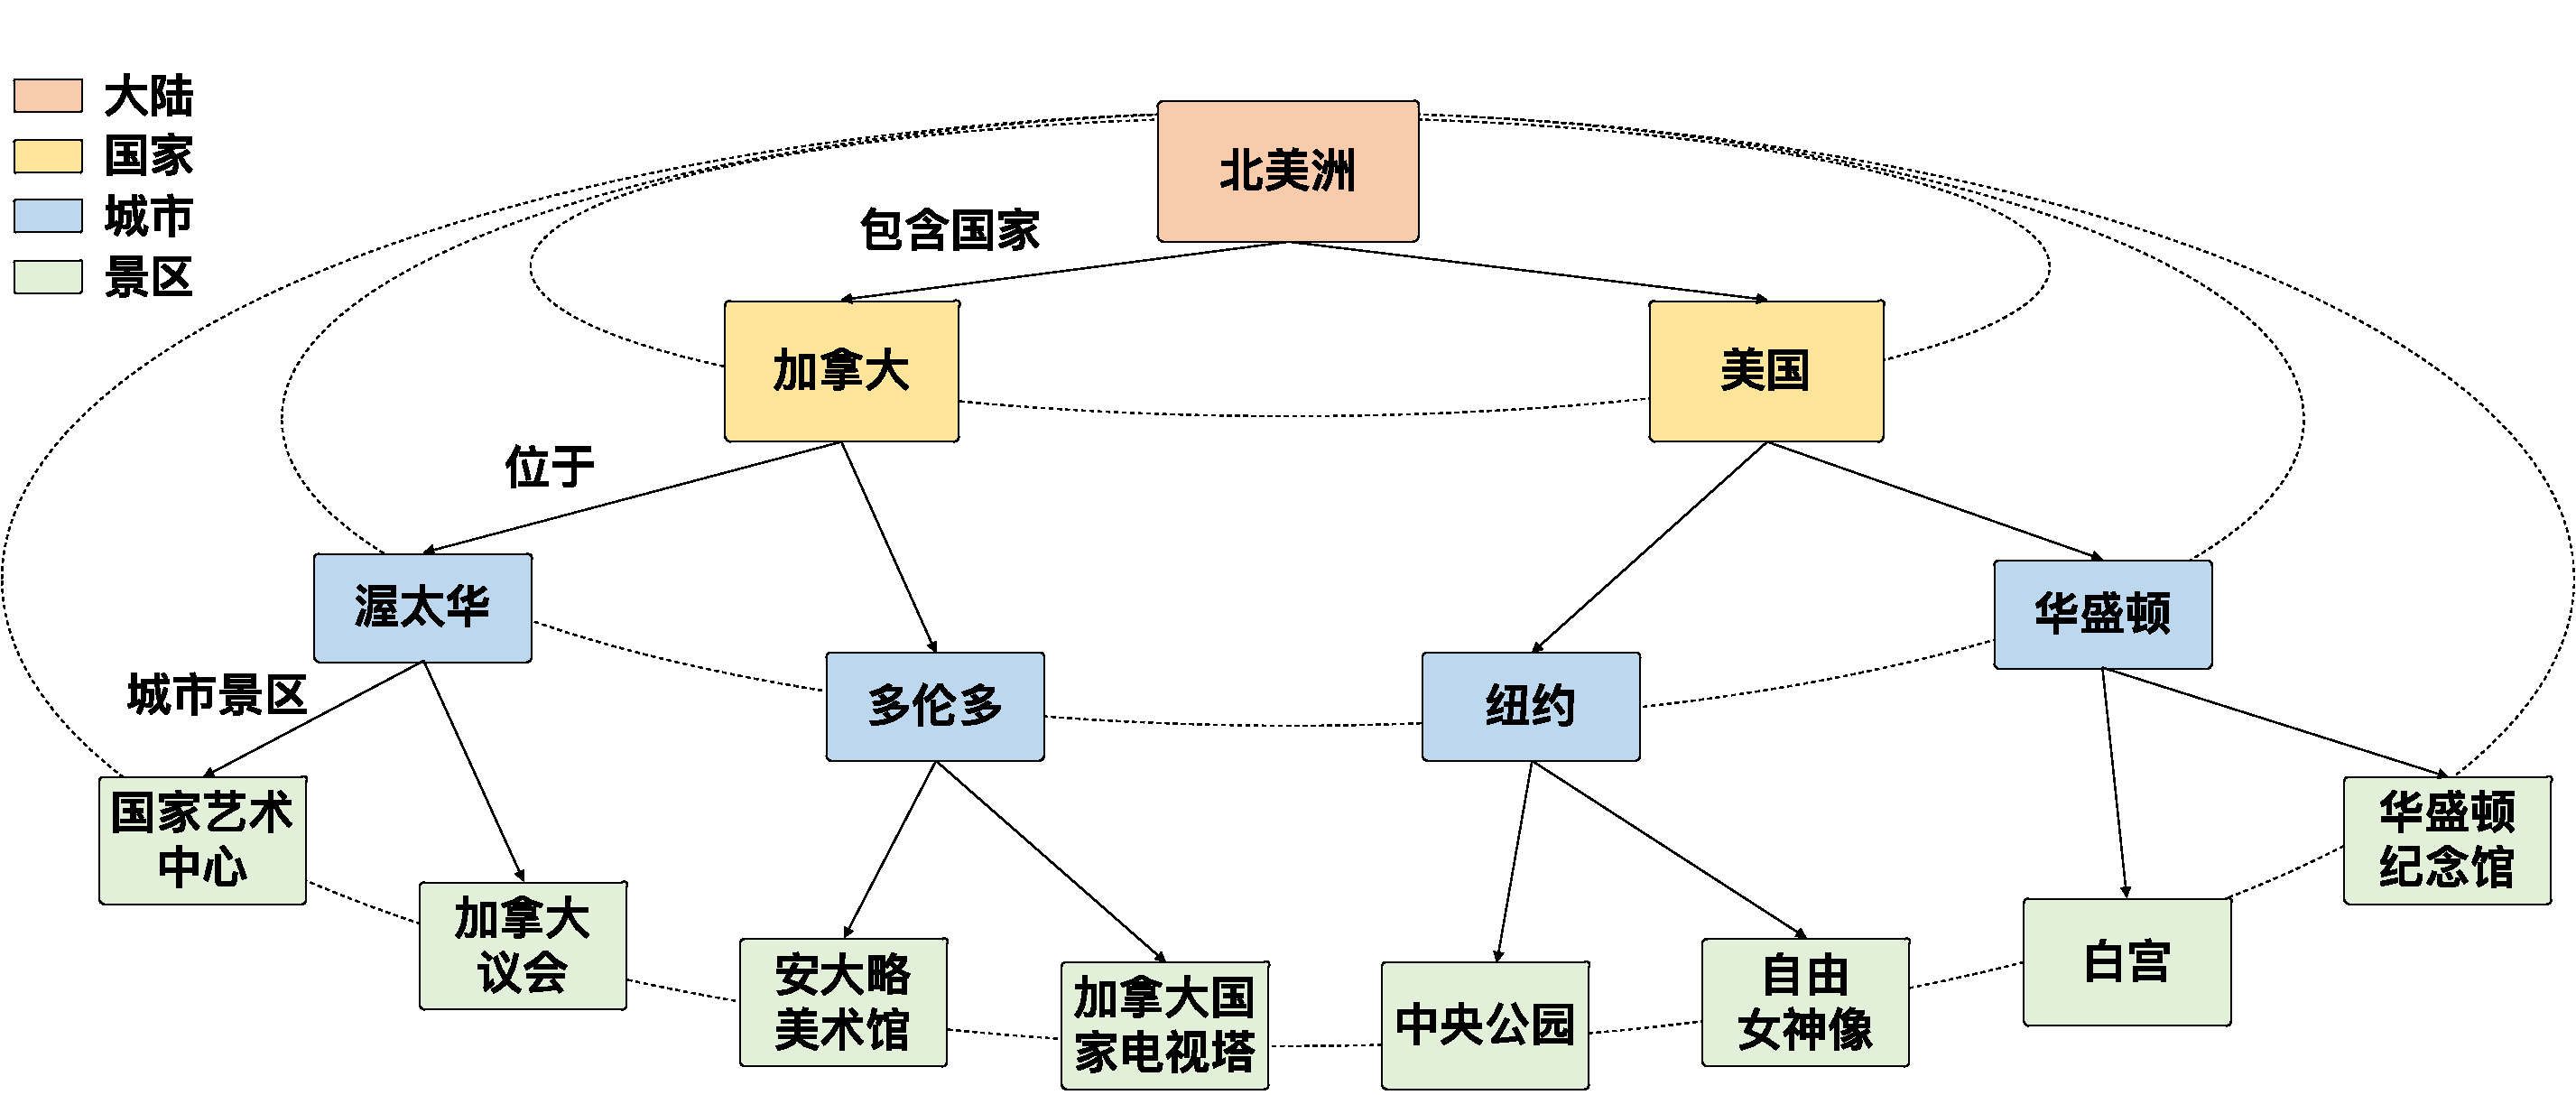
\includegraphics[width=0.9\textwidth]{1_KG}
  \caption{知识图谱}
  \label{1_KG}
\end{figure}

在实践中,知识图谱旨在作为组织或社区内不断发展的知识共享基础。知识图谱可以分为两类,分别是通用知识图谱和领域知识图谱~\cite{hogan2021knowledge}。两类知识图谱的原理相同,区别在于知识范围和应用领域,两种知识图谱在国内外均已得到广泛应用。国外的通用知识图谱包括百科知识图谱Freebase~\cite{bollacker2007platform},DBpedia~\cite{lehmann2015dbpedia}和Yago~\cite{hoffart2011yago2},多语言百科知识图谱Wikidata~\cite{vrandevcic2014wikidata},词典知识图谱WordNet~\cite{miller2007wordnet}和常识知识图谱CYC~\cite{lenat1995cyc}等。国内的通用知识图谱则包括中文百科知识图谱Zhishi.me~\cite{niu2011zhishi},该知识图谱首先采用固定的抽取规则,从百度百科、互动百科和中文维基百科中抽取实体信息,随后对不同百科的实体进行对齐,从而完成实体链接。CN-DBpedia~\cite{xu2017cn}是复旦大学开发的大规模通用领域结构化百科,从中文百科类网站的纯文本信息中提取信息,经过过滤、融合、推断等步骤后构成高质量结构化数据。领域知识图谱主要服务于特定行业领域,随着知识图谱在工业界的推广,逐渐发挥着越来越重要的作用。国外的领域知识图谱包括服务网络搜索的Google~\footnote{https://blog.google/products/search/introducing-knowledge-graph-things-not/}知识图谱,服务社交网络的LinkedIn~\footnote{https://engineering.linkedin.com/blog/2016/10/building-the-linkedin-knowledge-graph}知识图谱,服务商业领域的Aribnb~\footnote{https://medium.com/airbnb-engineering/scaling-knowledge-access-and-retrieval-at-airbnb-665b6ba21e95}和Amazon~\footnote{https://www.aboutamazon.com/news/innovation-at-amazon/making-search-easier}知识图谱,以及服务金融领域的Banca d’Italia~\cite{bellomarini2019knowledge}知识图谱等。国内的领域知识图谱包括百度~\cite{wang2013xlore}、淘宝~\cite{xu2021alime}、微博~\cite{wei2020analysis}等企业的知识图谱。由于领域知识图谱涉及到具体而复杂的领域场景,需要业务和开发专家的配合,因此对领域知识图谱的设计和开发提出了更高的要求。

知识图谱能够采用简洁的表示形式,将复杂多样的知识转化为清晰的三元组形式,并提供了强大的知识存储和推理能力。然而,知识图谱的知识信息通常采用自然语言进行描述,难以被计算机所处理和应用。因此,为了方便知识图谱的后续应用,需要将知识图谱内的知识信息转换为计算机能够直接处理的向量形式,这项技术被称为知识图谱表示学习(Knowledge Graph Representation Learning, KGRL)~\cite{chen2022rlpath}或知识图谱嵌入(Knowledge Graph Embedding, KGE)~\cite{wang2021transet}。知识图谱表示学习模型能够将知识图谱中的实体和关系映射到低维稠密的向量空间进行表示,同时保留其中的结构和语义信息,从而能够进行知识推理等知识应用工作。知识图谱表示学习主要涉及四个问题:(1)选择何种表示空间:现有的模型采用的表示空间可以分为欧氏空间~\cite{lu2022dense}、流形空间~\cite{ebisu2018toruse}、复向量空间~\cite{trouillon2016complex}和黎曼空间~\cite{pan2021hyperbolic}。(2)采用何种评分函数:现有的评分函数包括基于距离的评分函数~\cite{sachan2020knowledge}和基于语义相似度的评分函数~\cite{xiao2017ssp}。(3)应用何种编码模型:现有模型采用的编码模型包括线性模型~\cite{peng2020lineare}、双线性模型~\cite{pan2021hyperbolic}、因式分解模型~\cite{ji2015knowledge}和神经网络模型~\cite{jiang2021kernel}。(4)是否采用辅助信息,以及采用何种辅助信息:可以加入文本信息、视觉信息和类型信息等多种辅助信息~\cite{wang2017knowledge}。通过知识图谱表示学习,可以将知识信息转换为向量表示,作为知识图谱补全等下游任务的输入。由于知识图谱通常是采用自动或半自动的方式进行构建,因此通常是不完整的。通过现有知识预测知识图谱中缺失的知识,进行知识图谱补全,是提高知识图谱质量的有效手段~\cite{vu2019capsule}。

知识图谱的典型应用包括知识图谱补全和知识图谱问答。尽管知识图谱表示学习能够完成部分知识图谱补全和知识图谱问答的工作,但无法对关系路径进行建模,而只能基于单个实体或者关系进行简单的补全或问答,如进行单跳知识图谱问答。同时,知识图谱表示学习通过向量计算的方法进行隐式的知识补全,本质上属于黑盒模型,无法提供充分的证据,可解释性比较差。因此,需要借助知识图谱上的知识推理方法,综合考虑知识图谱网络图的拓扑结构信息对复杂关系路径进行建模,从而解决更为复杂的知识图谱补全和知识图谱问答内容,如实现多跳知识图谱问答,并提供相应推理证据~\cite{chen2020review}。知识推理不局限于传统的基于逻辑的和规则的推理方法,还可以采用更多样化的推理方法,随着技术的发展,一系列新的知识推理方法不断涌现,例如随机游走方法~\cite{jagvaral2020path}、路径排序方法~\cite{zhao2021target}、启发式方法~\cite{he2021heuristic}和神经网络方法~\cite{wang2018deep}等。丰富的知识图谱内容为知识推理技术的发展提供了新的机遇和挑战。

综上所述,知识图谱在人工智能应用中具有较大价值,面向知识图谱的表示学习技术有助于将知识图谱转化成易于处理和应用的知识图谱表示向量,并为下游任务提供充分的支持。知识推理是知识图谱智能应用的一个重要任务,深入研究该任务,有助于加深对知识图谱的认知,并充分和有效地利用知识图谱的知识。因此,本文旨在提出一种有效的知识图谱表示学习模型,随后基于知识图谱表示学习模型,实现一种知识推理模型,在适用于大规模知识图谱的前提下保证知识推理的质量,并能够解决诸如知识图谱补全、单跳知识图谱问答、多跳知识图谱问答和稀疏知识图谱上的知识图谱问答等知识推理任务。

\section{研究现状}
本节对面向知识图谱的表示学习和知识推理方法进行介绍,并介绍了一些常见的知识推理应用,此外还针对现有工作的问题进行了分析。

\subsection{知识图谱表示学习研究现状}
知识图谱能够有效地表示知识图谱中的结构化数据,但是难以被计算机进行直接处理和利用,需要先通过知识图谱表示学习的过程将知识三元组转换为向量的形式,才能应用于各类知识图谱推理任务。知识图谱可以表示为$G=\{E, R, F\}$,其中$E$、$R$和$F$分别表示实体、关系和事实的集合。知识图谱内的事实三元组可以表示为$(h, r, t) \in F$,其中$h$、$r$和$t$分别表示头实体、关系和尾实体。例如,对于给定的事实三元组(\textit{美国,首都,华盛顿特区}),其中的\textit{美国}是头实体$h$,\textit{华盛顿特区}是尾实体$t$,\textit{首都}则是头实体和尾实体之间的关系$r$。同时根据定义,有$h \in E$,$t \in E$,$r \in R$,以及$(h, r, t) \in F$。经过知识图谱表示学习后,可以将知识图谱中的节点和关系映射到低维稠密向量空间中。
这里使用粗体字符表示知识图谱表示向量,并设置目标向量空间为$d$维的欧氏空间,则完成知识表示后的实体和关系向量有$\bm{e} \in \mathbb{R}^{\mathrm{d}}$和$\bm{r} \in \mathbb{R}^{\mathrm{d}}$。欧氏空间是一种常用的向量空间,在实际的知识图谱表示学习任务中需要根据模型的需要来设置向量空间。为了构建知识图谱表示学习模型,需要完成三个步骤:(1)定义实体和关系在向量空间的表示形式。在这一步中,需要选择向量空间,设计编码模型,并确定是否需要辅助信息。(2)定义评分函数$f_r(h, t)$,用于评价知识$(h, r, t)$的合理性。知识图谱中可见事实三元组的得分一般会高于潜在事实三元组的得分。以及(3)学习实体和关系的表示,使知识图谱中可见事实三元组的总置信度最大化。

目前的知识图谱表示学习模型可以分为翻译模型,语义匹配模型和因果推断模型。

\subsubsection{翻译模型}
翻译模型采用基于距离的评分函数,将关系看做头实体和尾实体之间的翻译,并将关系翻译后两个实体之间的距离作为得分,进而实现衡量事实三元组的合理性。

翻译模型的典型代表是Bordes等人提出的TransE模型~\cite{bordes2013translating},其思想源于Mikolov等人提出的词嵌入模型word2vec~\cite{toms2013},在该模型中发现了词向量空间中存在平移不变性。例如TransE将知识图谱中的实体和关系映射到$d$维欧氏空间中,即$\bm{h}, \bm{r}, \bm{t} \in \mathbb{R}^{\mathrm{d}}$,并将关系看做是实体之间的连接向量,遵循$\bm{h} + \bm{r} \approx \bm{t}$,例如$\bm{h}$(\textit{美国}) $+ \bm{r}$(\textit{首都}) $\approx \bm{t}$(\textit{华盛顿特区})。同时对于给定三元组$(h, r, t)$,通过计算向量$\bm{h} + \bm{r}$和$\bm{t}$之间的$L1$或$L2$距离,进而得到三元组的合理性得分。对于较为合理的三元组,其得分应尽量接近0,对于不合理的三元组则希望其得分相对较低。TransE模型采用的得分函数可以表示为:$f_r(h, t) = - \|\bm{h} + \bm{r} - \bm{t}\|_{\ell_1 / \ell_2}$。尽管TransE模型在大规模知识图谱表示学习方面取得了巨大进步,但在处理如一对多、多对一和多对多等复杂关系时仍然存在困难。例如给定两个三元组(\textit{北京,所属国家,中国})和(\textit{上海,所属国家,中国}),可以发现它们是多对一类型的关系,即多个城市可以所属于同一个国家。根据TransE模型的要求$\bm{h} + \bm{r} \approx \bm{t}$,则实体\textit{北京}和\textit{上海}会被映射到向量表示空间中十分接近的位置。然而这两个实体实际上存在较大差异,因而这种映射是不合理的。

为了更好地处理复杂关系问题,Wang等人提出的TransH模型~\cite{wang2014knowledge}扩展了原始的TransE模型,为每种关系分别构建关系超平面,从而让一个实体在不同的关系超平面中会得到不同的表示向量。对于关系$r$,TransH会采用关系$r$独有的平移向量$\bm{d}_r$和超平面法线向量$\bm{w}_r$对关系进行表示。对于给定三元组$(h, r, t)$,TransH首先将$h$和$t$的表示向量沿着法线向量$w_r$的方向映射到关系超平面,设$\bm{h}_\perp$和$\bm{t}_\perp$分别为头实体和尾实体的映射向量,则有$\bm{h}_{\perp} = \bm{h} - \bm{w}_r^{\top} \bm{h} \bm{w}_r$,$\bm{t}_{\perp} = \bm{t} - \bm{w}_r^{\top} \bm{t} \bm{w}_r$。随后用关系平移向量$d_r$连接头实体向量和尾实体向量。TransH模型的评分函数为$f_r(h, t) = -\left\|\bm{h}_{\perp} + \bm{d}_r - \bm{t}_{\perp}\right\|_2^2$。虽然TransH模型使得实体能够根据关系获得不同表示,但全部实体和关系仍然在分布在相同的特征空间$\mathbb{R}^{\mathrm{d}}$中。由于实体具有多种语义,而不同关系可能关注实体的不同语义,因此单个特征空间可能不足以反映实体和关系的这一性质。

为了解决上述问题,Lin等人提出的TransR~\cite{lin2015learning}进一步扩展了TransH,将关系超平面扩展到了关系空间,即为每种关系构建对应的关系空间。对于给定三元组$(h, r, t)$,TransR将实体$h$和$t$映射到实体向量空间$\mathbb{R}^{\mathrm{d}}$中,同时为每个关系设置了相应的投影矩阵$\mathbf{M_r} \in \mathbb{R}^\mathrm{k \times d}$,能够将实体向量映射到关系$r$对应的向量空间$\mathbb{R}^{\mathrm{k}}$。设$\bm{h_\perp}$和$\bm{t_\perp}$分别为头实体和尾实体的映射向量,则有$\bm{h}_{\perp}=\mathbf{M}_r \bm{h}$,$\bm{t}_{\perp} = \mathbf{M}_r \bm{t}$。TransR采用投影矩阵,因此时空复杂度高于TransE和TransH。Ji等人提出的TransD~\cite{ji2015knowledge}模型很好地改善了TransR模型存在的问题。TransD对给定三元组$(h, r, t)$中每个实体和关系都构建两组向量,其中一组向量用来表示实体或关系的含义信息,表示为$\bm{h, t} \in \mathbb{R}^{\mathrm{d}}$和$\bm{r} \in \mathbb{R}^{\mathrm{k}}$,另一个向量用于形成两个动态投影矩阵,表示为$\bm{h_p, t_p} \in \mathbb{R}^{\mathrm{d}}$和$\bm{r_p} \in \mathbb{R}^{\mathrm{k}}$。相应地,构建的动态投影矩阵为$\mathbf{M}_{r h} = \bm{r}_p \bm{h}_p^{\top} + \mathbf{I}$,$\mathbf{M}_{r t}=\bm{r}_p \bm{t}_p^{\top} + \mathbf{I}$,其中$\mathbf{I} \in \mathbb{R}^{\mathrm{k \times d}}$是单位矩阵。设$\bm{h_\perp}$和$\bm{t_\perp}$分别为头实体和尾实体的映射向量,则有$\bm{h}_{\perp}=\mathbf{M}_{r h} \bm{h}$,$\bm{t}_{\perp}=\mathbf{M}_{r t} \bm{t}$。通过构建动态投影矩阵,TransD降低了矩阵运算的时空复杂度。

上述模型主要目标在于通过改变实体和关系的表示空间,提高表示学习的效果。除此之外,还有一些研究者从评分函数和编码方式的角度入手改进模型。对于给定的三元组$(h, r, t)$,TransM~\cite{fan2014transition}将与关系相应的权重$\theta_r$相关联,并将评分函数定义为$f_r(h, t)=-\theta_r\|\bm{h} + \bm{r} - \bm{t}\|_{1 / 2}$。通过给一对多、多对一和多对多关系分配较低的权重,可以让向量$\bm{h} + \bm{r}$和$\bm{t}$之间留有更大的距离。MainfoldE~\cite{xiao2016one}将$\bm{h} + \bm{r} \approx \bm{t}$的要求弱化为$\|\bm{h} + \bm{d} - \bm{t}\|_2^2 \approx \theta_r^2$,从而将$t$映射到以$\bm{h} + \bm{r}$为中心,半径为$\theta_r$的超球体,而不再是靠近$\bm{h} + \bm{r}$的确切点。同时,MainfoldE的评分函数定义为$f_r(h, t) = -\left(\|\bm{h} + \bm{r} - \bm{t}\|_2^2 - \theta_r^2\right)^2$。TransA~\cite{xiao2015transa}在TransR的基础上,使用自适应马氏距离代替传统的欧氏距离,并定义评分函数为$f_r(h, t) = -(|\bm{h} + \bm{r} - \bm{t}|)^{\top} \mathbf{M}_r(|\bm{h} + \bm{r} - \bm{t}|)$,从而使模型在处理复杂关系时更加灵活。

\subsubsection{语义匹配模型}
语义匹配模型采用基于相似度的评分函数,通过分析实体和关系的向量空间表示捕获语义信息,进而评估事实的合理性。模型的核心方法是,首先将知识图谱中的事实三元组$(h, r, t)$转换为三维的二元张量$\mathbf{X} \in \mathbb{R}^{\mathrm{n \times m \times n}}$,其中n为实体数量,m为关系数量,张量的每个切片$\mathbf{X}_k(k=1,2, \ldots, m)$对应相应的关系,张量值$\mathbf{X}_{i j k}$代表事实三元组$\left(h_i, r_j, t_k\right)$是否存在于知识图谱中,如果为1则存在,为0则不存在。

RESCAL~\cite{nickel2011three}是语义匹配模型的典型代表,采用张量来表示知识图谱的结构。对于关系$r_k$,有张量切片$\mathbf{X}_k \approx \mathbf{A} \mathbf{R}_k \mathbf{A}^{\top}$,其中矩阵$\mathbf{A}$用于捕获实体的潜在语义表示,矩阵$\mathbf{R}_k$用于对头尾实体对的交互进行建模。对于给定的三元组$(h, r, t)$,RESCAL的评分函数定义为$f_r(h, t)=\bm{h}^{\top} \mathbf{M}_r \bm{t}$,其中$\bm{h}, \bm{t} \in \mathbb{R}^d$是实体的嵌入向量,$\mathbf{M}_r \in \mathbb{R}^\mathrm{d \times d}$表示关系中的潜在语义信息。通过张量分解的方法,RESCAL能够较好地捕获实体和关系的语义信息,并给出三元组的合理性得分。然而,RESCAL的计算复杂度比较高。为了改善模型的时空复杂度,DistMult~\cite{yang2015embedding}将$\mathbf{M}_r$限制为对角矩阵,即$\mathbf{M}_r=\operatorname{diag}(\bm{r}), \bm{r} \in \mathbb{R}^\mathrm{d}$。随后,评分函数被调整为$f_r(h, t)=-\bm{h}^{\top} \operatorname{diag}(\bm{r}) \bm{t}$。通过这样的转换,DistMult显著降低了算法复杂度,同时在实验结果上取得了提高。然而,DistMult对头实体和尾实体的计算是对称的。对此,ComplEx~\cite{trouillon2016complex}模型通过复数嵌入,能够在不对称关系中扩展DistMult模型。实体和关系被嵌入到了复数空间$\mathbb{C}^\mathrm{d}$中,同时评分函数被修改为$f_r(h, t)=\operatorname{Re}\left(\bm{h}^{\top} \operatorname{diag}(\bm{r}) \bar{t}\right)$,其中$\operatorname{Re}(\cdot)$表示复数值的实数部分,$\bar{t}$表示尾实体的复数共轭部分。通过该评分函数,具有不对称关系的三元组就可以根据实体的序列获取不同的分数。

另一种具有代表性的语义匹配模型是RotatE~\cite{sun2018rotate}。受欧拉恒等式$e^{i \theta}=\cos \theta + i \sin \theta$的启发,RotatE引入了旋转哈达玛积,它将关系视为复数空间中头实体到尾实体的旋转,对于给定的三元组$(h, r, t)$,RotatE的评分函数为$f_r(h, t) = \|\bm{h} \circ \bm{r} - \bm{t}\|$,其中$\circ$表示旋转哈达玛积。通过这种方式,RotatE具有较好地表示和推理能力,能够处理对称/反对称关系、自反关系和复合关系。然而,RotatE采用的旋转哈达玛积在处理部分三元组时存在局限性。例如,给定三元组(\textit{母亲},\textit{父亲},\textit{祖母})和(\textit{父亲},\textit{母亲},\textit{祖父}),RotatE计算时会判断\textit{父亲的母亲}与\textit{母亲的父亲}是逻辑等价的,并将\textit{祖母}和\textit{祖父}映射到向量空间中角度接近的位置,但这种推导显然是错误的。为了解决这一问题,QuatE~\cite{zhang2019quaternion}模型将RotatE从复数空间扩展到四维空间,并采用哈密尔顿积替换旋转哈达玛积,用于捕获实体和关系间的潜在语义关联。相应的评分函数为$f_r(h, t)=\bm{h} \otimes \bm{r}|\bm{r}|^{-1} \cdot \bm{t}$,其中$\otimes$表示哈密尔顿积。由于哈密尔顿积的前后算子不可交换,所以能够区分类似\textit{父亲的母亲}和\textit{母亲的父亲}这样的实体概念,从而较好地解决RotatE存在的问题。

\subsubsection{因果推断模型}
因果推断模型将因果推断方法引入知识图谱表示学习领域,主要思想是引入因果干预方法,增强模型的领域适应性,减少局部结构差异,从而提高模型的泛化能力。同时通过因果分析还能够确定知识图谱表示学习时哪些特征信息有助于进行实体和关系表示,并提高相应的信息权重,进而增强模型的表示效果。

Wang等人提出的NIC模型~\cite{wang2021neighborhood}将因果推断模型与知识图谱表示学习领域相结合,提高了表示效果。知识图谱表示学习模型通过设计表示空间、评分函数和编码模型,并考虑加入辅助信息,完成模型的构建。对于给定的三元组$(h, r, t)$,模型会通过评分函数$f_r\left(h, t\right)$给出三元组的合理性评分。在训练模型学习实体和关系的向量表示时,通常选择优化目标是使得知识图谱中已有三元组的评分尽可能比未出现的三元组评分更高。然而,训练过程中的评分主要用于进行结果排序,而不是作为三元组的置信度得分。这导致评分函数的效果下降,限制了知识图谱补全等知识推理工作的发展。例如,给定三元组$(h, r, t)$,常规知识图谱表示学习方法的评分函数$f_r\left(h, t\right)$得到相应评分为0.9,但该三元组的实际置信度得分只有0.3,即评分与置信度得分存在不匹配的问题。因此,为了解决上述问题,使得评分函数能够给出接近实际置信度的评分,NIC提出了一个基于因果干预的置信度评估方法,称为邻里干预一致性(Neighborhood Intervention Consistency,NIC),通过验证预测结果的稳定性来评估置信度分数,具体方法是调整实体向量在不同维度上的值,设置为集合$\{0, \operatorname{avg}(\bm{e}), \max (\bm{e}), \min (\bm{e})\}$中的任意一种,即可以取零值、平均值、最大值和最小值其中之一。如果调整所有特征中的权值会导致时间效率过低,因此NIC通过特征选择获取不同维度的贡献,贡献计算函数为$w_j=|E|^{-1} \sum_{i=0}^{|E|}\left(\mathbf{E}_{i, j}-\operatorname{avg}\left(\mathbf{E}_{:, j}\right)\right)^2$,并选择贡献最大的维度进行调整。完成调整后,观察模型的输出序列是否改变或者是否与原始序列匹配,匹配度计算方法为$\zeta\left(S, S^{N_i}\right)=\sum_{j=0}^J \sigma(S)_j\left(1-\operatorname{Sgn}\left(\left|\varrho(S)_j-\varrho\left(S^{N_i}\right)_j\right|\right)\right)$,其中$\sigma$和$\operatorname{Sgn}$分别为Softmax函数和Sign函数,该函数可以表示因果干预后预测结果的稳健性,并计算置信度得分为$p_{n i c}(S)=d^{-1} \sum_{i=0}^d\left(\varsigma\left(S, S^{N_i}\right)\right)$,是0到1之间的实数。

另一种具有代表性的因果推断知识图谱表示学习模型为Feng等人提出的CGI模型~\cite{feng2021should},采用图卷积神经网络。图卷积神经网络广泛应用于知识图谱表示学习中,其主要思想是通过聚合实体节点的邻域信息实现实体表示效果的增强。然而,由于知识图谱中局部结构属性存在较大差异,即存在局部结构差异问题,从而造成实体节点表示存在不一致分布的问题,这导致对不同节点使用相同的聚合方法会降低节点表示效果。通常的解决方案是采用注意力机制,通过训练降低可能导致局部结构差异的邻居的权重,然而通常无法实现理想情况的注意力机制效果。针对上述问题,CGI采用了因果图卷积神经网络模型,该模型能够根据局部结构的因果效应调整训练好的图卷积神经网络模型。CGI首先得到节点的原始表示向量,该向量受到邻域特征和自身特征的影响。随后采用因果干预,将邻域置位空,从而实现屏蔽图结构,并要求实体节点根据自身特征获取表示向量。因果干预过程可以表示为$e=f(x, \mathcal{N}(x) \mid \theta)-f(x, \operatorname{do}(N=\emptyset) \mid \theta)$,其中$\operatorname{do}(N=\emptyset)$表示执行因果干预,将邻域置为空集合。最后CGI根据局部结构的因果效应、预测置信度和其他因素,采用一个独立的二元分类器$D=\{(x, p) \mid \hat{z}=z \cup \hat{z}=z\}, p=\operatorname{flag}(\hat{z}=z)$,在因果干预表示和原始表示之间进行选择。实验证明模型通常能够在遇到局部结构差异时选择因果干预表示,即屏蔽邻域特征仅采用节点自身特征的表示。

\subsection{知识推理研究现状}
通过知识图谱表示学习模型可以通过知识图谱问答的方式实现知识推理,即给定查询语句,通过知识抽取技术获取对应的查询三元组$\left(h, r, ?\right)$,$\left(h, ?, t\right)$或$\left(?, r, t\right)$,通过将知识图谱内所有关系或实体作为候选答案,输入到知识图谱表示学习模型中,从而将实体与关系映射到低维向量空间中,并通过得分函数进行打分,随后根据得分结果进行排序,选择得分最高的实体或关系作为答案,并完成知识推理。然而,基于知识表示学习模型的推理在形式上只能完成单跳的推理,无法显式地进行多跳推理,因而无法提供推理路径。这使得推理过程缺乏可解释性~\cite{wang2019deeppath}。为了解决这一问题,提出了关系路径推理方法,该类方法利用知识图谱上的拓扑结构信息,在知识图谱的关系路径上进行建模和推理。采用关系路径推理的方式,不仅可以得到推理结果,同时还可以给出一个可解释的、采用推理路径作为引导的推理过程。

现有的知识推理模型可以分为符号逻辑推理模型,神经推理模型和神经符号混合推理模型。

\subsubsection{符号推理模型}
符号推理模型(Symbolic reasoning model)旨在为非结构化自然语言查询语句生成结构化的查询。现有的符号推理模型可以分为语义解析和基于模板的知识推理两种方法。其中,语义解析方法通过自然语言处理工具,将问题转换为句法依赖表示。基于模板的知识推理方法则构建大量模板,包括自然语言模式和相应的结构化查询模式(例如SPARQL),从而实现复杂问题的分解。

马尔可夫符号网络(Markov Logic Network, MLN)~\cite{richardson2006markov}是基于预定义的规则和知识图谱中的事实三元组信息构建的概率图模型,能够在模型训练的过程中学习不同规则的权重,最终。具体而言,给定一个具体的规则集合,其中的每个规则都可以通过知识三元组进行具体查询,则可以通过下列步骤完成MLN模型的构建:首先为每个规则对应的知识三元组构建一个对应节点,如果知识三元组存在则节点值设为1,否则设为0。随后如果两个节点如果对应同一个规则,则在两个节点之间构建一条边。最后令每个规则对应一个特征,如果规则成立则特征值为1,否则特征值为0。规则的所有节点都共享这个特征。完成MLN模型构建后,网络中所有节点的联合分布定义为$P(X=x)=Z^{-1} \exp \left(\sum_i w_i n_i(x)\right)$,其中$w_i$是对应规则的权重,是$n_i$规则对应节点的数量。随后可以通过MCMC算法进行MLN模型的推理,并通过优化伪似然度量实现权重的学习。基于学习的权重,即可以完成具体的路径推理。通过引入权重信息,MLN能够较好地将一阶谓词逻辑和概率图模型进行结合,并实现不确定性的推理。然而,知识图谱结构十分复杂,造成了MLN的推理非常困难且效率低下。此外,知识图谱中缺失的三元组也会影响规则推理的效果。为了解决上述问题,pLogicNet~\cite{qu2019probabilistic}综合了MLN和图嵌入技术的思想,首先通过MLN定义知识图谱中事实三元组的联合分布,并对每种逻辑规则与权重构建关联,随后采用变分EM算法有效地学习权重。在EM算法中,E步骤推断未观察到的三元组的合理性,其对应的变分分布采用TransE等知识图谱表示学习模型进行参数化,M步通过优化观察到的三元组和知识图谱表示学习模型得到的三元组上的伪似然来更新逻辑规则的权重。通过上述方法,pLogicNet可以实现高效知识推理,同时能够处理知识图谱中缺失的信息。

另一类符号逻辑推理模型的代表是ProbLog~\cite{de2007problog},它是逻辑编程语言ProLog的一个改进。ProLog能够基于给定规则、事实和查询语句进行自动的知识推理并给出答案。ProbLog则是对于每种规则设置了一个概率,并令最终的知识推理给出推理的概率,从而模拟知识推理过程中的不确定性。给定查询,则推理概率被定义为$P\left(q \mid T\right)=\sum_{L \in L_T} P(q, L \mid T)$,其中T描述了原因L的概率分布,因此推理概率被分解为查询的所有联合概率和每种可能的原因集合的总和。其中有$P(q, L \mid T)=P(q \mid L) \cdot P(L \mid T)$,进一步分解了推理概率,其中$P(L \mid T)$表示给定原因的情况下查询的概率,如果至少有一个答案能够使查询为真,则对应的$P(L \mid T)$的值为1。式中另一项,即原因集合的概率的计算方法为$P(L \mid T)=\prod_{c_i \in L} p_i \prod_{c_i \in L_r \backslash L}\left(1-p_i\right)$。为了计算$P(L \mid T)$,一种方法是枚举所有可能的逻辑规则和对应的事实,效率较低。另一种方法是采用ProLog的选择线性确定(Selective Linear Definite,SLD)方案,采用自上而下的方式构造SLD树。首先通过查询步骤初始化根节点,随后通过应用每个规则及对应的事实来递归创建子目标,到达结束条件时停止迭代,即找到了查询目标或到达了树的最大深度。同时,每种查询结果都与一系列带有概率的规则相关联。

\subsubsection{神经推理模型}
神经推理模型的推理方法是将知识图谱中的实体、关系和查询问题共同编码到相同的表示空间中,并在表示空间中进行知识推理。传统的基于距离和基于语义匹配的模型无法满足知识推理的要求,为了获得更加有效的实体和关系嵌入效果,神经推理模型引入了神经网络结构,用于知识图谱邻域信息的建模。神经推理模型与知识图谱表示学习模型比较相似,都是首先进行知识图谱表示,随后实现知识推理等任务,但不同在于,神经推理模型会将自然语言查询问题也编码到表示空间中,从而增强知识推理的效果。同时,神经推理模型能够处理单跳知识图谱问答、多跳知识图谱问答和复杂逻辑问答问题,而知识图谱表示学习模型通常只能处理单跳知识图谱问答问题。

ConvE~\cite{dettmers2018convolutional}是第一种采用卷积神经网络的神经推理模型,首先将头实体和关系映射到向量空间,随后将向量转换成矩阵并进行拼接,输入到卷积层中。ConvE采用二维卷积捕获两个实体之间的特征交互信息,并通过卷积层和全连接层获取实体之间不同维度的局部信息,返回特征图张量。随后,将张量转化为向量,并投影到向量空间,最后通过计算与尾实体向量的内积,得到最终的合理性得分。其评分函数为$f_r\left(h, t\right)f(\operatorname{vec}(f([\bm{h} ; \bm{r}] \times \omega)) \mathbf{W}) t$,其中$\omega$为卷积核,$\mathbf{W}$为权重矩阵。此外,ConvE还引入了一个一对多的评分程序,能够自动匹配所有尾实体,从而能够更有效率地评估所有候选答案尾实体。然而,ConvE将实体和关系向量转换为矩阵并进行拼接,这一过程丢失了翻译模型的平移不变性。对此,ConvKB~\cite{nguyen2018novel}去除了ConvE的转换操作,并采用一维卷积保持平移不变性,同时捕获实体之间的全局关系和平移特征。ConvKB将每个三元组$(h, r, t)$的d维度嵌入表示为一个三列的矩阵$(\bm{h}, \bm{r}, \bm{t}) \in \mathbb{R}^{\mathrm{d} \times 3}$,随后将矩阵输入到卷积层,其中提供许多相同维度的过滤器,能够提取三元组中相同维度特征之间的全局关系,并通过对矩阵的每行进行操作以获得不同的特征图,最后将这些特征图拼接成一个三元组特征向量,并通过和权重矩阵进行点积运算得到最终的三元组合理性得分,评分函数为$f_r(h, t)=\operatorname{concat}(g([\bm{h}, \bm{r}, \bm{t}] \times \Omega)) \cdot \mathbf{W}$,其中$g$为激活函数,$\Omega$为过滤器,$\mathbf{W}$为权重矩阵。HypER~\cite{balazevic2019hypernetwork}是基于ConvE提出的又一种卷积神经网络推理模型,采用基于ConvE的超网络为每个关系生成卷积滤波器权重,超网络可以实现跨层的权重共享,并动态生成给定输入的权重。HypER使用基于特定关系的一维卷积滤波器来处理实体嵌入,这简化了嵌入模式。同时,HypER使用卷积算子实现头实体嵌入和一组特定于关系的滤波器$F_r$,滤波器是超网络$H$从关系嵌入中创建的,超网络的结构是一个全连接层。最后,HypER还应用了ReLU激活函数的权重矩阵$\mathbf{W}$实现特征图张量的向量化。HypER的评分函数为$f_r(h, t)=f\left(\operatorname{vec}\left(\bm{h} \times F_r\right) \mathbf{W}\right) \bm{t}$,相较于ConvE,HypER具有更强的表达能力和更少的参数。

传统的神经推理模型通过单向关系路径或文本信息引入上下文信息,而忽略了实体之间的各种连接模式,以及不重要的路径和词的影响,这造成模型无法充分捕捉三元组之间的关系信息。为了解决这一问题,R-GCN~\cite{schlichtkrull2018modeling}采用关系图卷积网络,显式地对多关系知识图谱进行建模并捕获实体周围的单跳邻域事实信息。R-GCN由编码器和解码器构成,在对实体进行编码的时候,R-GCN能够综合考虑实体连接之间的各类输入和输出的关系信息,并对实体的结构信息进行充分的编码。实体表示被更新为$\bm{h}_i^{(l+1)}=\sigma\left(\sum_{r \in R} \sum_{j \in \mathbf{N}_i^r} c_{i, r}^{-1} \mathbf{W}_r^{(l)} \bm{h}_j^{(l)}+\mathbf{W}_0^{(l)} \bm{h}_i^{(l)}\right)$,其中$\mathbf{N}_i^r$是节点i在关系$r \in R$下的邻域,$c_{i,r}$是特定问题的归一化常数。解码时,可以通过基数分解和块对角矩阵分解的方法求解,并选择DistMult分解模型作为评分函数,认为每个关系都对应一个对角矩阵,从而得到最终的评分函数为$f_r(h, t)=\bm{h}^T \mathbf{R}_r \bm{t}$。R-GCN分析了知识图谱中邻域信息对实体表示的影响,但是没有显式地对实体间的关系进行建模。SACN~\cite{shang2019end}模型对R-GCN进行了改进,是一种加权的GCN模型,能够同时考虑节点间的连通性、节点的属性和关系类型。SACN同样由编码器和解码器构成。编码器部分,SCAN引入了不同类型关系的权重以对GCN模型进行改进,得到加权图神经网络。同时,在聚合信息时对不同类型的关系分别进行聚合,因此可以将多关系图按照多个单关系图的形式进行分析。此外,SACN还将实体属性作为属性节点加入到了实体表示部分,并采用类似的方法进行分析。在SACN模型中,实体表示被更新为$h_i^{l+1}\sigma\left(\sum_{j \in \mathbf{N}_i} \alpha_t^l \bm{h}_j^l \mathbf{W}^l+\bm{h}_i^l \mathbf{W}^l\right)$。解码器采用Conv-TransE进行解码,利用卷积过滤器直接对相同维度的实体和关系向量进行处理。

\subsubsection{神经符号推理模型}
神经符号推理模型(Neural-symbolic reasoning model)是符号推理模型和神经推理模型的结合,综合了两种模型的优点。现有的神经符号推理模型包括神经增强符号推理模型(Neural-enhanced symbolic reasoning model)和端到端推理模型。其中,神经增强符号推理模型仅仅用于将问题解析成结构化的查询,随后需要使用查询方法才能够得到最终答案。而端到端推理模型可以自动完成解析问题并检索答案的步骤。

DeepPath~\cite{wang2019deeppath}首先将强化学习模型应用到了关系路径知识推理方面,并开发了一种新的奖励函数,通过综合分析模型是否到达目标节点、模型推理路径长度是否过长和与已有路径嵌入向量的相似度,来提高准确性、路径多样性和推理效率。DeepPath首先采用翻译模型的方法,对连续空间中的智能体状态信息进行编码,并选择知识图谱的关系空间作为强化学习模型的动作空间。另一种基于强化学习的模型是MINERVA~\cite{das2018go},根据基于LSTM的策略网络对邻域信息进行采样。同时,与DeepPath不同的是,MINERVA中的状态是由查询关系和部分路径的嵌入组成,在采样的过程中不需要答案实体的嵌入向量,从而能够允许MINERVA直接通过知识推理得到答案。同时,MINERVA还为知识图谱的每个节点增加了自关系,从而能够在推理过程中在到达答案实体时自动停止。然而DeepPath和MINERVA在分析模型是否到达目标节点时,提供的奖励机制比较简单,即如果智能体到达目标节点则提供值为1的奖励,同时对没有达到目标节点的情况提供值为-1的惩罚或者值为0的奖励。这种方法导致了奖励稀疏问题并降低了模型探索路径的效果。对此,Multi-Hop模型~\cite{lin2018multi}改进了强化学习的奖励函数,将硬奖励替换成了基于真实答案实体和推理实体之间相似度的软奖励。同时,受到dropout技术的启发,Multi-Hop在模型训练的过程中丢弃了一些动作,从而避免选择大量重复路径,缓解过拟合问题。另一种缓解奖励稀疏的方法由M-Walk~\cite{shen2018m}模型提出,该模型采用了一种基于价值的强化学习方法,并使用蒙特卡洛树搜索(Monte Carlo Tree Search,MCTS)来客服奖励稀疏的问题。具体而言,M-Walk迭代地使用MCTS的轨迹生成步骤和策略改进步骤,实现细化策略网络,从而获得更多的奖励信息。

除去关系路径知识推理模型,另一种神经符号推理模型采用图结构进行推理。GraIL模型~\cite{teru2020inductive}采用图神经网络的形式,并在提取的子图上推理两个实体之间的关系。具体而言,GraIL首先提取头实体和尾实体周围的k跳子图并取交集,随后采用元组$(d(i, h), d(i, t))$标记子图中的实体,其中$i$表示子图中的第$i$个节点,$d$表示头实体和尾实体到节点的最短距离。随后采用基于注意力的多关系图神经网络,也就是R-GCN,计算每个节点的实体表示,最后将头实体、尾实体和查询关系的表示向量连接起来,并以此为基础在子图上进行推理。GraIL在学习与实体无关的关系语义方面具有很强的能力。CogGraph~\cite{du2019cognitive}从给定的头实体和查询关系开始,通过策略网络在每一步扩展多个实体,随后采用GNN模型获取节点在推理子图中的表示向量,并预测答案。DPMPN模型~\cite{xu2019dynamically}采用了两个图神经网络模型来执行推理。第一个模型在整个知识图谱上进行消息传递,用于提供实体表示。第二个模型在查询子图上修建消息传递图,用于捕获与查询相关的语义。

此外,还有基于矩阵的神经符号推理模型。这种模型可以看做图神经网络模型的扩展,其不会基于跳数选择邻居,而是综合软注意力分数来评估不同邻居的重要性。其基本思想是通过矩阵运算来表达头尾实体之间的重要性。TensorLog~\cite{cohen2016tensorlog}是较早提出的基于矩阵的模型,能够通过知识推理,得到带有权重的链式逻辑规则,从而解释知识图谱中的每个关系。随后基于推理得到的规则,输入头实体和关系,目标是通过检索对实体进行排名,将正确答案尽可能排在靠前的位置。TensorLog采用独热向量表示实体,并用矩阵表示知识图谱中的向量,其中如果知识存在于知识图谱中,则矩阵对应位置为1。但是,TensorLog中的参数较难学习,因为每种规则都对应一个参数,而枚举规则本身就是一个离散的任务。对此,神经逻辑编程(NeuralLP)模型~\cite{yang2017differentiable}将规则的权重参数分解为了规则中谓词的权重。同时,设计了一个循环公式来动态建模规则的长度。最后,NeuralLP计算所有向量的加权平均值,并使用注意力来控制规则的长度。上述两种方法可以学习一些概率链式逻辑规则,但是无法推断出一些复杂的规则形式,如树状规则。此外,链式规则是基于特定的头实体进行推断的,这也会降低学习的泛化性。对此,神经逻辑归纳学习(Neural Logic Inductive Learning, NLIL)模型~\cite{yang2019learn}将原始语句进行合并以处理非链式规则,并取得较好的效果。

\subsection{知识推理应用}
通过知识图谱表示学习模型,可以得到知识图谱内实体和关系的表示向量。随后通过知识推理模型,可以进一步利用知识表示向量内的信息,从而实现一系列知识推理应用。常见的知识推理应用主要包括知识图谱补全和知识图谱问答。

\subsubsection{知识图谱补全}
知识图谱补全(Knowledge Graph Completion,KGC)~\cite{vu2019capsule}指的是预测与实体有相应关系的实体的任务,即给定头实体$h$和关系$r$预测对应的尾实体$t$,或是给定关系$r$和尾实体$t$预测对应的头实体$h$,前者可以表示为查询三元组$\left(h, r, ?\right)$,后者可以表示为查询三元组$\left(?, r, t\right)$,这种类型的知识图谱补全任务被称为实体预测。类似的,另一种知识图谱补全任务是给定头实体$h$和尾实体$t$并预测关系$r$,可以表示为查询三元组$\left(h, ? t\right)$,这种知识图谱补全被称为关系预测。以查询尾实体为例,给定查询三元组$\left(h, r, ?\right)$,首先选择在知识图谱表示学习模型,将头实体$h$和关系$r$映射到向量空间中,随后可以选择将知识图谱中每个实体作为候选答案,并使用得分函数$f_r\left(h, t\right)$计算三元组得分。随后,将按照得分从高到低的顺序获取候选答案的有序序列,并检查正确答案在序列中的位置。评价知识图谱补全的好坏主要在于正确答案在最终候选答案序列中的位置是否靠前,通常采用的评价指标有平均排序MR(正确答案排名的平均值)、平均倒数排序MRR(正确答案排名倒数的平均值)以及Hits@K(正确答案在序列中排名位于前K的比例)等。

\subsubsection{知识图谱问答}
知识图谱问答(Knowledge Graph Question Answering,KGQA)包括单跳知识图谱问答、多跳知识图谱问答和复杂逻辑问答等多种形式~\cite{saxena2020improving}。其中,单跳知识图谱问答与知识图谱补全类似,两者的区别在于,知识图谱补全采用查询三元组的形式,提供两个已知元素并要求模型通过推理得到未知的元素,从而实现知识图谱补全。知识图谱问答则不提供查询三元组,而提供自然语言查询语句$q$,并要求模型基于该问句进行问题的解答,答案类型可以是实体和关系。相比之下,多跳知识图谱问答更加复杂,知识推理模型需要通过知识图谱上的多跳关键路径进行推理才能获得答案实体和关系,同时部分多跳问答数据集如HotpotQA还要求模型提供相应的证据来证明推理的有效性~\cite{yang2018hotpotqa}。复杂逻辑问答提供的查询语句中包含多个主题实体,主题实体之间通过连接词$\land$、析取词$\vee$和否定词$\neg$进行聚合,因此可以对每个主题词进行多跳推理,最后对推理结果进行求交集,获取最终答案。知识图谱问答的常见解决方案是,首先对查询语句$q$进行实体识别,获取其中的主题实体,随后基于主题实体,可以采用知识图谱补全的方案,通过知识图谱表示学习模型进行单跳知识推理,或采用基于关系路径的知识推理模型进行多跳知识推理和复杂逻辑推理,最终得到目标实体或关系,实现问题求解。评价知识图谱问答的效果可以分析正确答案在最终答案候选序列的位置是否靠前,可以采用的评价指标有平均排序MR、平均倒数排序MRR和Hit@K等。


\subsection{存在问题分析}
随着DBpedia、Freebase和Yago等一系列大规模知识图谱的提出,面向知识图谱的表示学习和知识推理的相关研究取得了重要进展。然而,尽管越来越多的模型在各种知识推理应用中取得了瞩目的效果,但仍然面临着许多挑战:

\begin{itemize}
  \item [1.]\textbf{模型对知识图谱层次信息的感知能力不强:}现有面向知识图谱的表示学习和知识推理模型通常能够较好的建模知识图谱内部三元组的语义信息,但是通常对知识图谱的层次信息建模能力较差,导致在进行知识图谱表示和知识推理的过程中无法充分利用知识图谱内丰富的层次信息,限制了模型效果。
  \item [2.]\textbf{模型难以分析和体现知识的因果性:}现有的知识图谱表示学习模型通常直接选择捕获目标知识的实体和邻域中的信息进行表示学习,而没有进行因果推断以避免邻域结构差异对表示结果的影响。同时知识图谱表示学习过程无法清晰地评估实体和邻域节点对表示结果的贡献程度,限制了模型在具体应用任务中的表现。
  \item [3.]\textbf{模型推理能力不足:}多跳推理任务和稀疏知识图谱上的推理任务在现实世界中十分常见,具有重要的研究和应用价值。然而现有的知识图谱推理模型对多跳推理和稀疏知识图谱上的推理的支持仍然较差,同时,采用知识图谱表示学习模型进行推理只能实现单跳推理,这限制了知识图谱表示学习模型在知识推理应用上的进一步应用。
  \item [4.]\textbf{模型可解释性较差:}采用神经网络结构的知识推理模型,由于模型结构可以理解为黑盒模型,所以难以分析模型得出结果的具体过程。同时如果采用知识图谱表示学习模型直接进行知识推理,则模型只会得出推理结果,而不会提供相应的推理路径和证据信息,这导致难以分析模型推理的具体过程进而优化模型。
  \item [5.]\textbf{知识图谱表示学习模型与知识推理模型的结合不够充分:}由于通常情况下知识图谱表示学习模型与知识推理模型的训练过程相互分离和缺乏协作,导致模型间的结合不够充分,从而降低了面向知识图谱的知识推理的效果。
\end{itemize}

\section{论文工作}
针对现有的面向知识图谱的表示学习和知识推理方法存在的问题,本文提出了知识图谱表示学习模型NORMAN(k\textbf{NO}wledge graph \textbf{R}epresentation learning \textbf{M}odel based on c\textbf{A}usal i\textbf{N}ference)和知识推理模型LAURA(know\textbf{L}edge graph re\textbf{A}soning model based on d\textbf{U}al-agent \textbf{R}einforcement le\textbf{A}rning)。
NORMAN模型首先获取知识图谱中的层次级别和知识表示向量,随后将它们作为输入提供给图神经网络模型进行模型训练,并在训练过程中将因果推断方法融入信息传递过程中以提高模型的稳定性,最终完成知识图谱表示学习模型的训练,得到的模型能够将知识转换为向量表示,并可以为知识推理过程提供支持。
LAURA模型利用NORMAN模型提供的层次信息和知识表示向量作为输入,训练实体级和层次级两种粒度的强化学习推理模型,并通过协作动作空间、协作策略网络和轨迹相似度奖励实现实体级和层次级知识推理模型的信息交互和轨迹协调,最终完成知识图谱推理模型的训练,得到的模型可以根据给定知识信息进行推理,返回知识推理答案、知识推理路径和置信度信息。

\begin{figure}
  \centering
  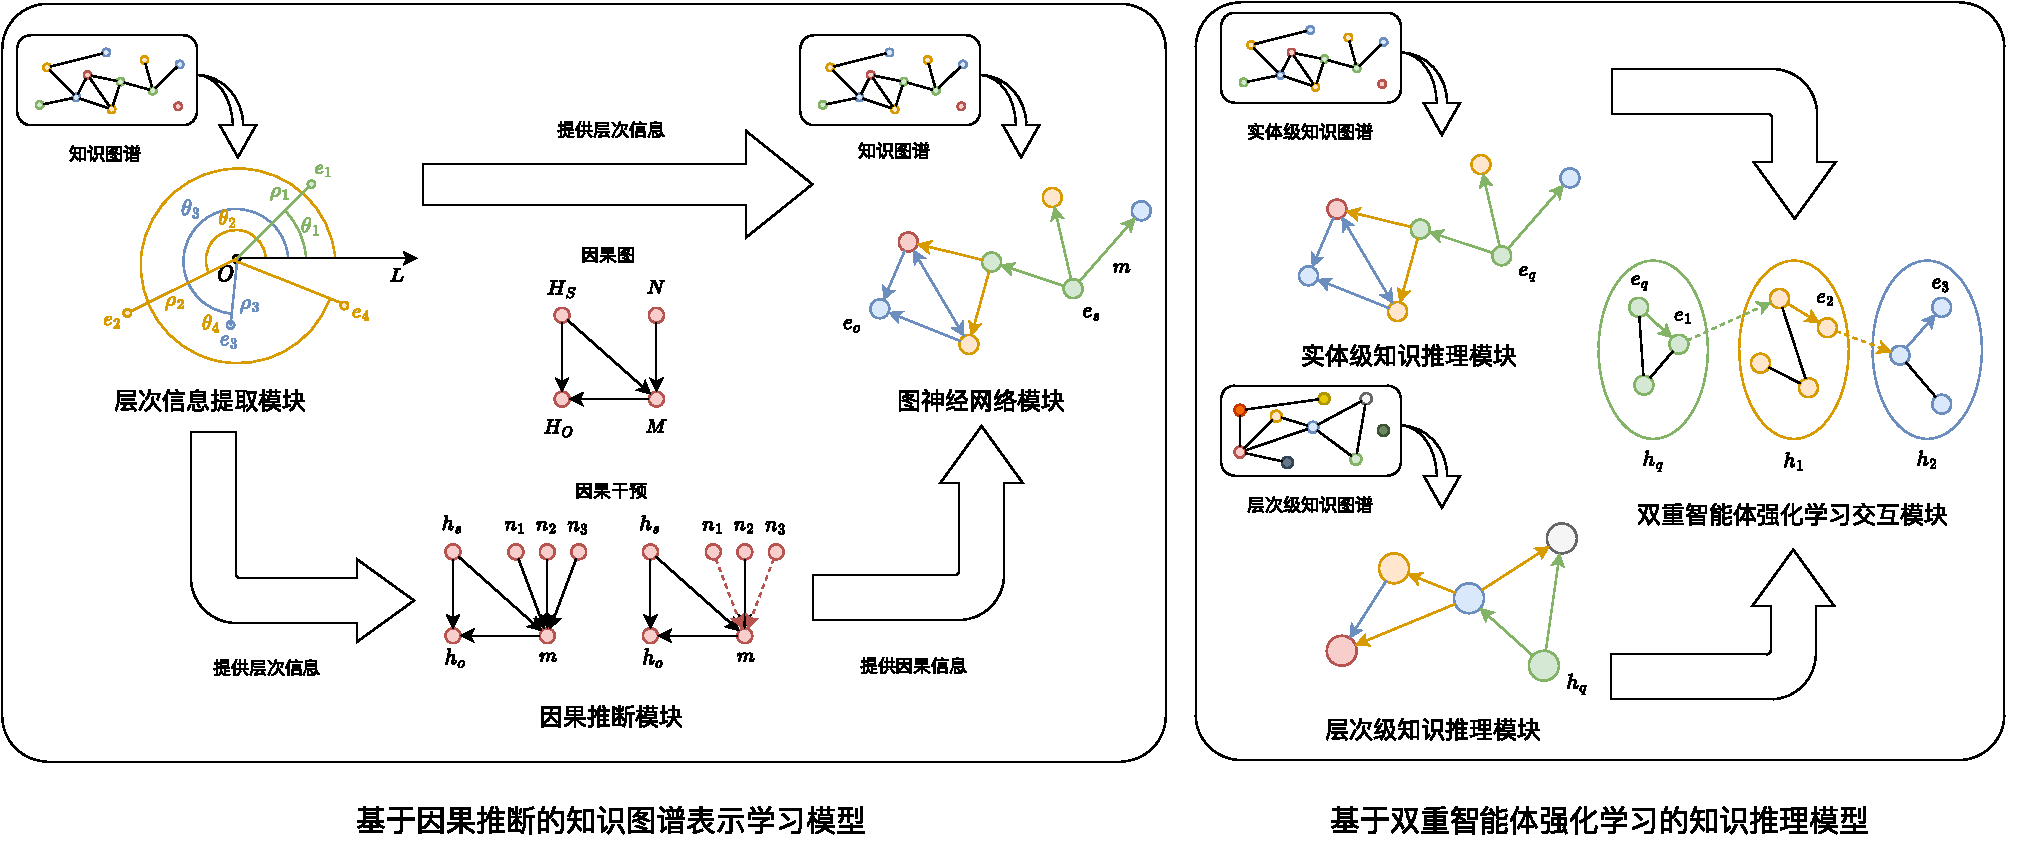
\includegraphics[width=0.9\textwidth]{1_Total}
  \caption{技术路线图}
  \label{1_Total}
\end{figure}
本文的整体技术路线图如图\ref{1_Total}所示。从整体上看,本文首先研究基于因果推断的知识图谱表示学习,能够捕获知识图谱的语义信息、邻域信息和层次信息,并通过因果推断提高知识表示的效果,通过构建并训练知识图谱表示学习模型,将知识信息转换为向量信息,并为知识推理提供支持。随后研究基于双重智能体强化学习的知识推理,构建实体级和层次级强化学习模块,通过知识图谱表示学习模型增强模块能力,并通过双重智能体强化学习交互模块实现两个模块的信息交流和轨迹协调,最后通过训练模型实现高质量和高可解释性的知识推理模型。本文的主要工作包括:

\begin{itemize}
  \item [1.]\textbf{提出一种基于因果推断的知识图谱表示学习模型:}该模型包含层次信息提取模块、因果推断模块和图神经网络模块。
  层次信息提取模块的目标是增强模型对层次信息的利用能力,提高模型对知识信息的表示效果。本文采用极坐标表示法编码知识图谱,并以半径坐标作为知识的层次信息,角坐标则用于区分相同层次的知识。通过对半径坐标进行聚类,可以实现对知识的层次信息提取,为因果推断模块提供数据支持。
  因果推断模块能够将因果推断融入知识图谱表示学习中,评估邻域信息是否有助于进行表示和推理并进行取舍。本文采用邻域信息因果干预的方法,综合考虑层次差异得分、决策差异得分、预测置信度得分和推理距离得分等多种因素,判断当前节点是否接收来自邻域节点的信息。本文通过加入因果推断方法,提高知识图谱表示效果,为知识推理提供充分支持。
  图神经网络模块采用图神经网络模型,构建的图神经网络模型能够充分利用知识图谱中各个实体的邻域结构信息,并通过知识邻域间的信息传递进行数据更新。在此过程中,模块利用层次信息提取模块的层次信息作为辅助,采用因果推断模块评估是否接收邻域信息。完成训练后的模型,能够将输入的知识结构化三元组转换为表示向量,并可以用于后续知识推理工作。
  在公开数据集上的实验结果表明,本文提出的NORMAN模型在知识图谱补全任务上优于现有模型。
  \item [2.]\textbf{提出一种基于双重智能体强化学习的知识推理模型:}该模型包含实体级强化学习模块、层次级强化学习模块和双重智能体强化学习交互模块。
  模型采用强化学习框架,能够根据知识图谱中的拓扑结构进行多跳推理,并能够通过显式推理生成推理路径,提高知识推理的可解释性。通过融合知识图谱表示学习模型,知识推理模型能够对动作空间进行扩展,从而缓解了知识图谱稀疏性问题。通过利用知识图谱表示学习的评分函数作为软奖励提供给没有到达目标节点的推理过程,缓解了强化学习的奖励稀疏问题,提高了模型的学习速度和推理能力。
  在知识推理过程中,实体级和层次级强化学习模块能够分别根据知识图谱中的实体和层次信息进行知识推理,实现微观和宏观两种粒度的知识推理。
  同时,双重智能体强化学习交互模块用于实现上述两种粒度的强化学习模块的合作。通过采用协作动作空间、协作策略网络和轨迹相似度奖励,能够实现模块间的信息交互和轨迹协调,实现高质量和高可解释性的知识推理。
  在公开数据集上的实验结果表明,本文提出的LAURA模型在单跳和多跳知识图谱问答任务上优于现有模型。
\end{itemize}


\section{论文组织结构}
本文共分为五章,各章的主要内容如下:

第一章为论文的绪论部分,首先对论文的研究背景进行了介绍,随后分别从面向知识图谱的表示学习模型和知识推理模型两种角度进行分析,并给出了当前知识推理的主要应用,最后分析了当前面向知识图谱的表示学习和知识推理方法存在的问题,并引出了本文工作。

第二章提出了一种基于因果推断的知识图谱表示学习模型NORMAN。首先介绍知识图谱表示学习任务,随后进行模型框架概览,并对模型的三个模块进行详细介绍,随后针对模型开展实验评估,最后对模型进行总结。

第三章提出了一种基于双重智能体强化学习的知识推理模型LAURA。首先介绍知识推理任务,随后完成模型框架概览,对模型的三个模块进行详细介绍,随后对模型开展实验评估,最后对模型进行总结。

% 第四章为实验评估部分,首先介绍实验开展的环境,随后针对知识图谱表示学习模型和知识推理模型分别开展实验,依次介绍实验的评价指标、数据集、实验设置以及实验结果和分析,从而对本文提出的两种模型进行综合评价。

第四章对全文工作进行了总结,并展望了未来研究方向。


\chapter{基于因果推断的知识图谱表示学习模型}
本章提出一种基于因果推断的知识图谱表示学习模型NORMAN,主要包含三个模块,分别是层次信息提取模块、因果推断模块和图神经网络模块,该方法首先通过极坐标编码模型捕获知识图谱的层次信息,随后通过图神经网络模型进行知识图谱表示,并在模型训练过程中利用因果推断方法提高知识表示效果。
本章主要包含七个部分:知识图谱表示学习任务定义(2.1节),模型方法概览(2.2节),层次信息提取模块(2.3节),因果推断模块(2.4节),知识图谱嵌入模块(2.5节),实验评估(2.6节),以及本章小结(2.7节)。

\section{知识图谱表示学习任务定义}
知识图谱能够将知识表示为结构化三元组的形式,这种形式能够清晰准确地表示各种实体信息以及实体之间的关系,同时能够方便研究人员实现知识信息的可视化展示,有助于对知识信息进行直观地研究。但是,结构化三元组难以直接与各类机器学习模型结合起来,并用于解决知识图谱补全和知识图谱问答等下游任务。因此,需要通过知识图谱表示学习的方式,将知识图谱中的结构化三元组表示为向量形式,进而应用于各类知识图谱下游任务。
知识图谱可以表示为$G=\{E, R, F\}$,其中$E$、$R$和$F$分别表示实体、关系和事实的集合。知识图谱内的事实三元组可以表示为$(h, r, t) \in F$,其中$h$、$r$和$t$分别表示头实体、关系和尾实体。同时根据定义,有$h \in E$,$t \in E$,以及$r \in R$。
经过知识图谱表示学习后,可以将知识图谱中的节点和关系映射到低维稠密向量空间中,从而可以用于多种知识图谱下游任务。使用粗体字符表示知识图谱表示向量,则完成知识表示后的三元组为$\left(\bm{h}, \bm{r}, \bm{t}\right) \in \mathbb{R}^{\mathrm{d}}$,这里假定知识表示的向量空间为维度是$d$维的欧氏空间,根据模型的需要,也可以投影到其他类型的向量空间。总的来说,知识图谱表示学习任务目的在于构建知识图谱表示学习模型,能够捕获知识图谱中的关键信息,为下游任务提供数据支持。

通常情况下,知识图谱表示学习模型主要包含以下三个组成部分,分别是:
\begin{itemize}
  \item [1.] 实体和关系的表示空间。现有的研究工作中,表示空间包含点空间、流空间、复向量空间、高斯分布和离散空间等。
  \item [2.] 用于评估知识三元组合理性的评分函数。评分函数主要可以分为基于距离的和基于相似度匹配的评分函数。
  \item [3.] 用于学习将实体和关系编码成向量形式的编码模型。编码模型是当前研究的重点内容,主要包括线性、双线性、矩阵分解和神经网络等多种类型。
\end{itemize}

此外,知识图谱表示学习模型还可以补充其他用于提高表示模型效果的辅助信息,包括文本、视觉和听觉等多种模态的相关信息。
在具体的模型构建与训练过程中主要包含以下三个步骤:
\begin{itemize}
  \item [1.] 定义实体和关系在向量空间的表示形式。在这一步中,需要选择向量空间,设计编码模型,并确定是否需要辅助信息。
  \item [2.] 定义评分函数。评分函数可以表示为$f_r(h, t)$,用于评价知识$(h, r, t)$的合理性。一般而言,知识图谱中已知的事实知识三元组的得分会高于潜在事实三元组的得分。
  \item [3.] 学习实体和关系的表示,使知识图谱中可见事实三元组的总置信度最大化。
\end{itemize}

通过上述训练步骤,能够得到一个有效的知识图谱表示学习模型,该模型能够将实体和关系表示为向量的形式,并能够用于各类知识图谱下游任务。
其中本章涉及到的相关符号及定义如表\ref{2_symbols}所示。
\begin{table}
  \centering
  \begin{tabular*}{0.8\textwidth}{@{\extracolsep{\fill}}clcl}
		\toprule[1pt]
    符号 & 描述 & 符号 & 描述 \\ \hline
    $\mathbb{R}^{\mathrm{d}}$ & $d$维欧氏空间 & $h$ & 节点信息变量\\
    $\|\cdot\|_{p}$ & $p$范数 & $v_h$ & 层次差异得分\\
    $\circ$ & 哈达玛积运算 & $v_d$ & 决策差异得分\\
    $\bmod$ & 求余运算 & $v_c$ & 预测置信度得分\\
    $E(\cdot)$ & 期望计算 & $v_l$ & 推理距离得分\\
    $\rho$ & 半径坐标 & $\alpha$ & 注意力权重\\
    $\theta$ & 角坐标 & $D$ & 数据集合\\
    $Y$ & 潜在结果 & $\lambda$ & 权重\\
    $X$ & 背景变量 & $\epsilon$ & 聚类最大步数\\
    $W$ & 处理 & $\gamma$ & 固定边界值\\
    $P$ & 分配概率 & $K$ & 层次类别数\\
    $n$ & 邻域节点变量 & $L$ & 最大消息传递距离\\
    $m$ & 聚合消息变量 & & \\
    % $h$ & 节点信息变量\\
    % $v_h$ & 层次差异得分\\
    % $v_d$ & 决策差异得分\\
    % $v_c$ & 预测置信度得分\\
    % $v_l$ & 推理距离得分\\
    % $\alpha$ & 注意力权重\\
    % $G_{neighbor}$ & 知识图谱邻域子图\\
    % $D$ & 数据集合\\
    % $\lambda$ & 权重\\
    % $\epsilon$ & 聚类最大步数\\
    % $\gamma$ & 固定边界值\\
    % $K$ & 层次类别数\\
    % $L$ & 最大消息传递距离\\
		\bottomrule[1pt]
	\end{tabular*}
  \caption{本章符号定义}
  \label{2_symbols}
\end{table}

\section{基于因果推断的知识图谱表示学习模型框架概览}
本章提出的NORMAN模型可以根据知识图谱的结构信息和关联情况,将原始的实体和关系数据转换为特征向量。图\ref{2_NORMAN}展示了该模型,模型主要包含三个模块,分别是层次信息提取模块、因果推断模块和图神经网络模块。
对于层次信息提取模块,需要将知识图谱中的知识三元组数据作为输入。模块使用欧氏空间作为知识表示空间,采用基于距离的评分函数,并选择极坐标系编码模型获取知识的表示向量。同时,模块还会提取知识表示向量中的半径坐标,并通过聚类算法获取知识对应的层次级别。模块的输出包括知识表示向量和知识层次级别两部分内容。
对于因果推断模块,在模型训练过程中需要将知识表示向量提供给因果推断模块,该模块采用邻域信息因果干预的方法,综合考虑层次差异得分、决策差异得分、预测置信度得分和推理距离得分等多种因素,评估各个图神经网络节点是否接收来自邻域节点的信息,并输出评估结果。
对于图神经网络模块,该模块为知识图谱表示学习模型的主体部分,采用图神经网络模型,在训练过程中将层次信息提取模块的知识向量作为对应知识的初始状态,并通过知识邻域间的消息传递进行数据更新,同时使用因果推断模块评估各个图神经网络节点是否接收特定邻域的信息。完成训练后的模型能够将输入的结构化知识转换为表示向量,并用于后续的知识推理工作。
\begin{figure}
  \centering
  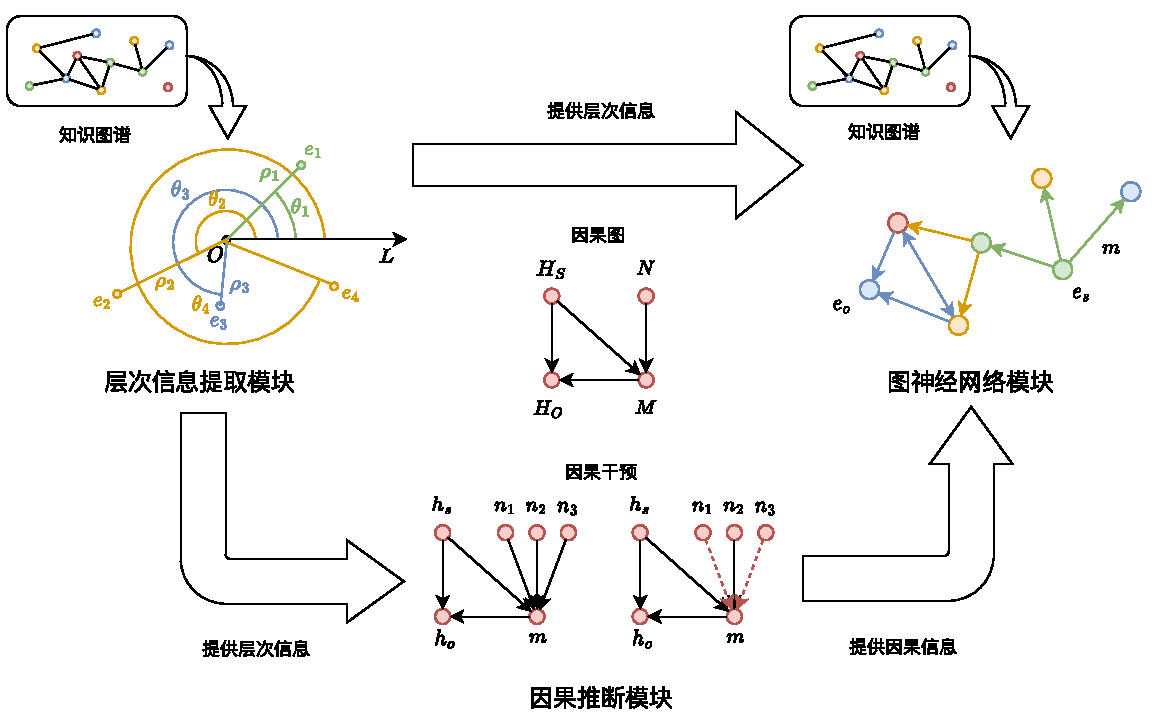
\includegraphics[width=0.9\textwidth]{2_NORMAN}
  \caption{基于因果推断的知识图谱表示学习模型框架图}
  \label{2_NORMAN}
\end{figure}

\section{层次信息提取模块构建}
层次信息在知识图谱中非常常见,例如在图\ref{1_KG}中的知识图谱上就包含了四种层次级别的实体,分别是大陆、国家、城市和景区,这些实体的层次级别呈现从高到低的排列。同时,不同层次级别的实体之间存在着不同关系,这些关系同样存在层次级别,例如图中存在三种关系,按照关系的层次级别由高到低的顺序排列,分别是包含国家、位于和城市景区。
同时,知识图谱中的实体类型和关系类型存在长尾分布的情况。以FB15K-237知识图谱为例,图谱的实体类型和关系类型的知识数量分布情况如图\ref{2_LongTail}所示。可以发现知识图谱中的一小部分实体类型对应了大部分的知识数据,而大部分实体类型则只有很少的知识数据。同时可以发现,关系类型的知识数量分布分布情况也同样呈现长尾分布情况。
上述问题对模型的知识图谱表示能力提出了较高的要求,即模型需要能够表示知识图谱中的层次信息,同时还要考虑知识图谱中实体类型和关系类型的知识数量呈现长尾分布的特点,能够对不同类型的实体和关系进行区分。
对此,本文构建了层次信息提取模块,能够在捕获知识图谱层次信息的同时对不同关系类型进行区分,提高知识图谱表示学习模型的效果。
% 这就需要模型要有较强的表达能力,能够区分相同层次的不同实体与关系,同时尽量减少表示误差。
% 需要注意的是,一般情况下位于高层次级别知识数量相对较少,位于低层次级别的知识数量则相对更多。例如FB15K-237知识图谱的关系类型和知识数量的分布情况如图\ref{2_LongTail}所示,可以发现关系类型数量呈现长尾分布的情况,只有少量关系类型的知识数量较多,更多关系类型则对应的知识数量相对较少。同时对于关系类型进行分析,可以发现知识数量多的关系对应的层次级别一般较高,例如超过五千条知识的关系类型包括了\textit{Profession}和\textit{LocationContains}等高层次关系类型,相应的,知识数据量少的关系类型则集中在低层次级别。这就需要模型要有较强的表达能力,能够区分相同层次的不同实体与关系,同时尽量减少表示误差。
\begin{figure}
  \centering
  \subfloat[实体类型的知识数量分布情况]{
    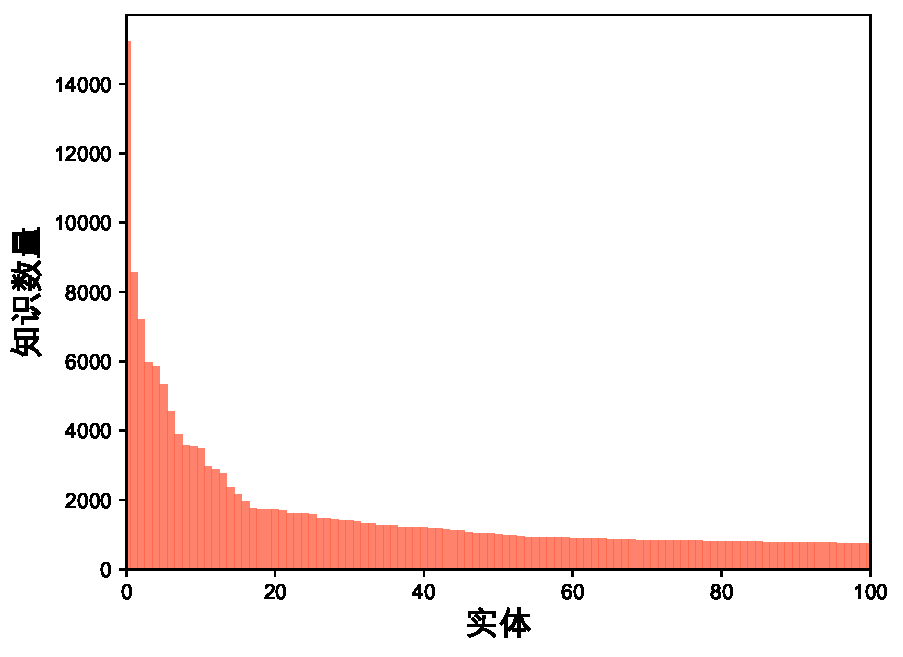
\includegraphics[width=0.4\textwidth]{2_LongTail_a.pdf}
    \label{2_LongTail_a}
  }
  \subfloat[关系类型的知识数量分布情况]{
    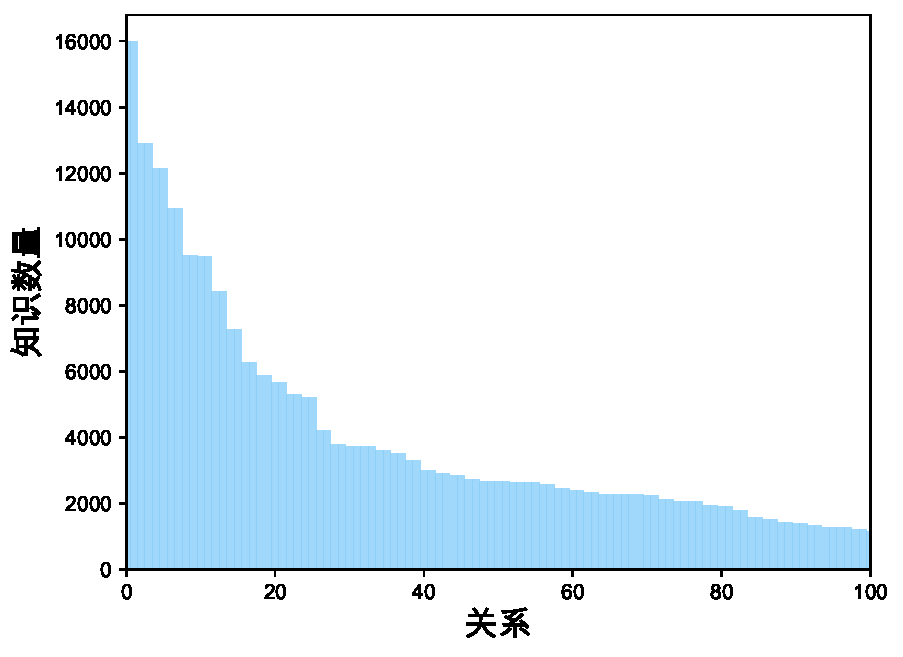
\includegraphics[width=0.4\textwidth]{2_LongTail_b.pdf}
    \label{2_LongTail_b}
  }
  \caption{知识图谱实体类型和关系类型的长尾分布情况}
  \label{2_LongTail}
\end{figure}

在介绍层次信息提取模块的过程中,本节首先介绍了层次信息提取模块概览,给出了层次信息提取模块的结构图。随后介绍了模块采用的极坐标系编码模型,并给出了编码知识图谱的过程。最后介绍了对半径坐标进行聚类的过程,总结了模块的输出信息。

\subsection{层次信息提取模块概览}
现有的知识图谱表示学习模型主要侧重于建模对称、反对称、逆向和组成等关系模式,然而,许多模型无法表示知识图谱中的层次信息,这限制了模型的表示能力。为了应对这一挑战,本文设计了层次信息提取模块。
如任务定义中介绍,选择实体和关系的编码模型是知识图谱表示学习任务的关键。在具体的选择过程中需要结合一定的先验知识,从而设计出可以更好地捕获知识图谱语义与结构信息的编码模型。如图\ref{1_KG}中所示,对知识图谱的结构进行分析可以发现,知识图谱中的实体与关系存在的层次信息可以表示为类似同心圆的结构,在该结构中靠近圆心的部分是层次级别较高的实体和关系,远离圆心的部分则对应层次级别较低的实体和关系。
因此,为了更好地捕获知识图谱中的层次结构信息,本文选择使用极坐标系编码模型对知识图谱进行编码,这是因为极坐标系上任意一点的位置是根据其到极点的距离$\rho$(半径坐标)和其与极轴按照逆时针方向计算的角度$\theta$(角坐标)所唯一确定的。通过将知识图谱中层次级别较高的实体和关系映射到靠近极点(半径坐标模量较小)的位置,将层次较低的内容映射到远离极点(半径坐标模量较大)的位置,从而能够对知识图谱中的层次信息进行表示。同时,为了区分不同实体和关系,可以通过调整实体和关系的角坐标,尽量让节点能够均匀分布在圆周上,从而提高知识图谱表示效果。上述思路在具体实现的过程中主要是通过模块的评分函数进行实现的。
此外,在表示空间的选择方面,本文选择欧氏空间作为知识表示空间,主要是因为可以将极坐标系下的欧氏距离度量函数融入评分函数中,从而保证知识图谱表示学习过程的正确性。

综上所述,本节构建的层次信息提取模块的结构如图\ref{2_Layers}所示。可以发现,模块主要是采用极坐标系编码器将知识图谱映射到欧氏空间,并通过半径坐标区分不同层次的实体和关系,通过角坐标区分不同类型的实体和关系。
图中包含了四种不同类别的节点,但节点$e_2$和$e_4$的半径坐标模量相等,说明两个节点位于同一个层次。
完成模型训练的层次信息提取模块能够将知识转换成表示向量,同时能够通过半径坐标向量聚类的方式获取实体和关系的层次级别,从而可以为其他模块提供支持。
\begin{figure}
  \centering
  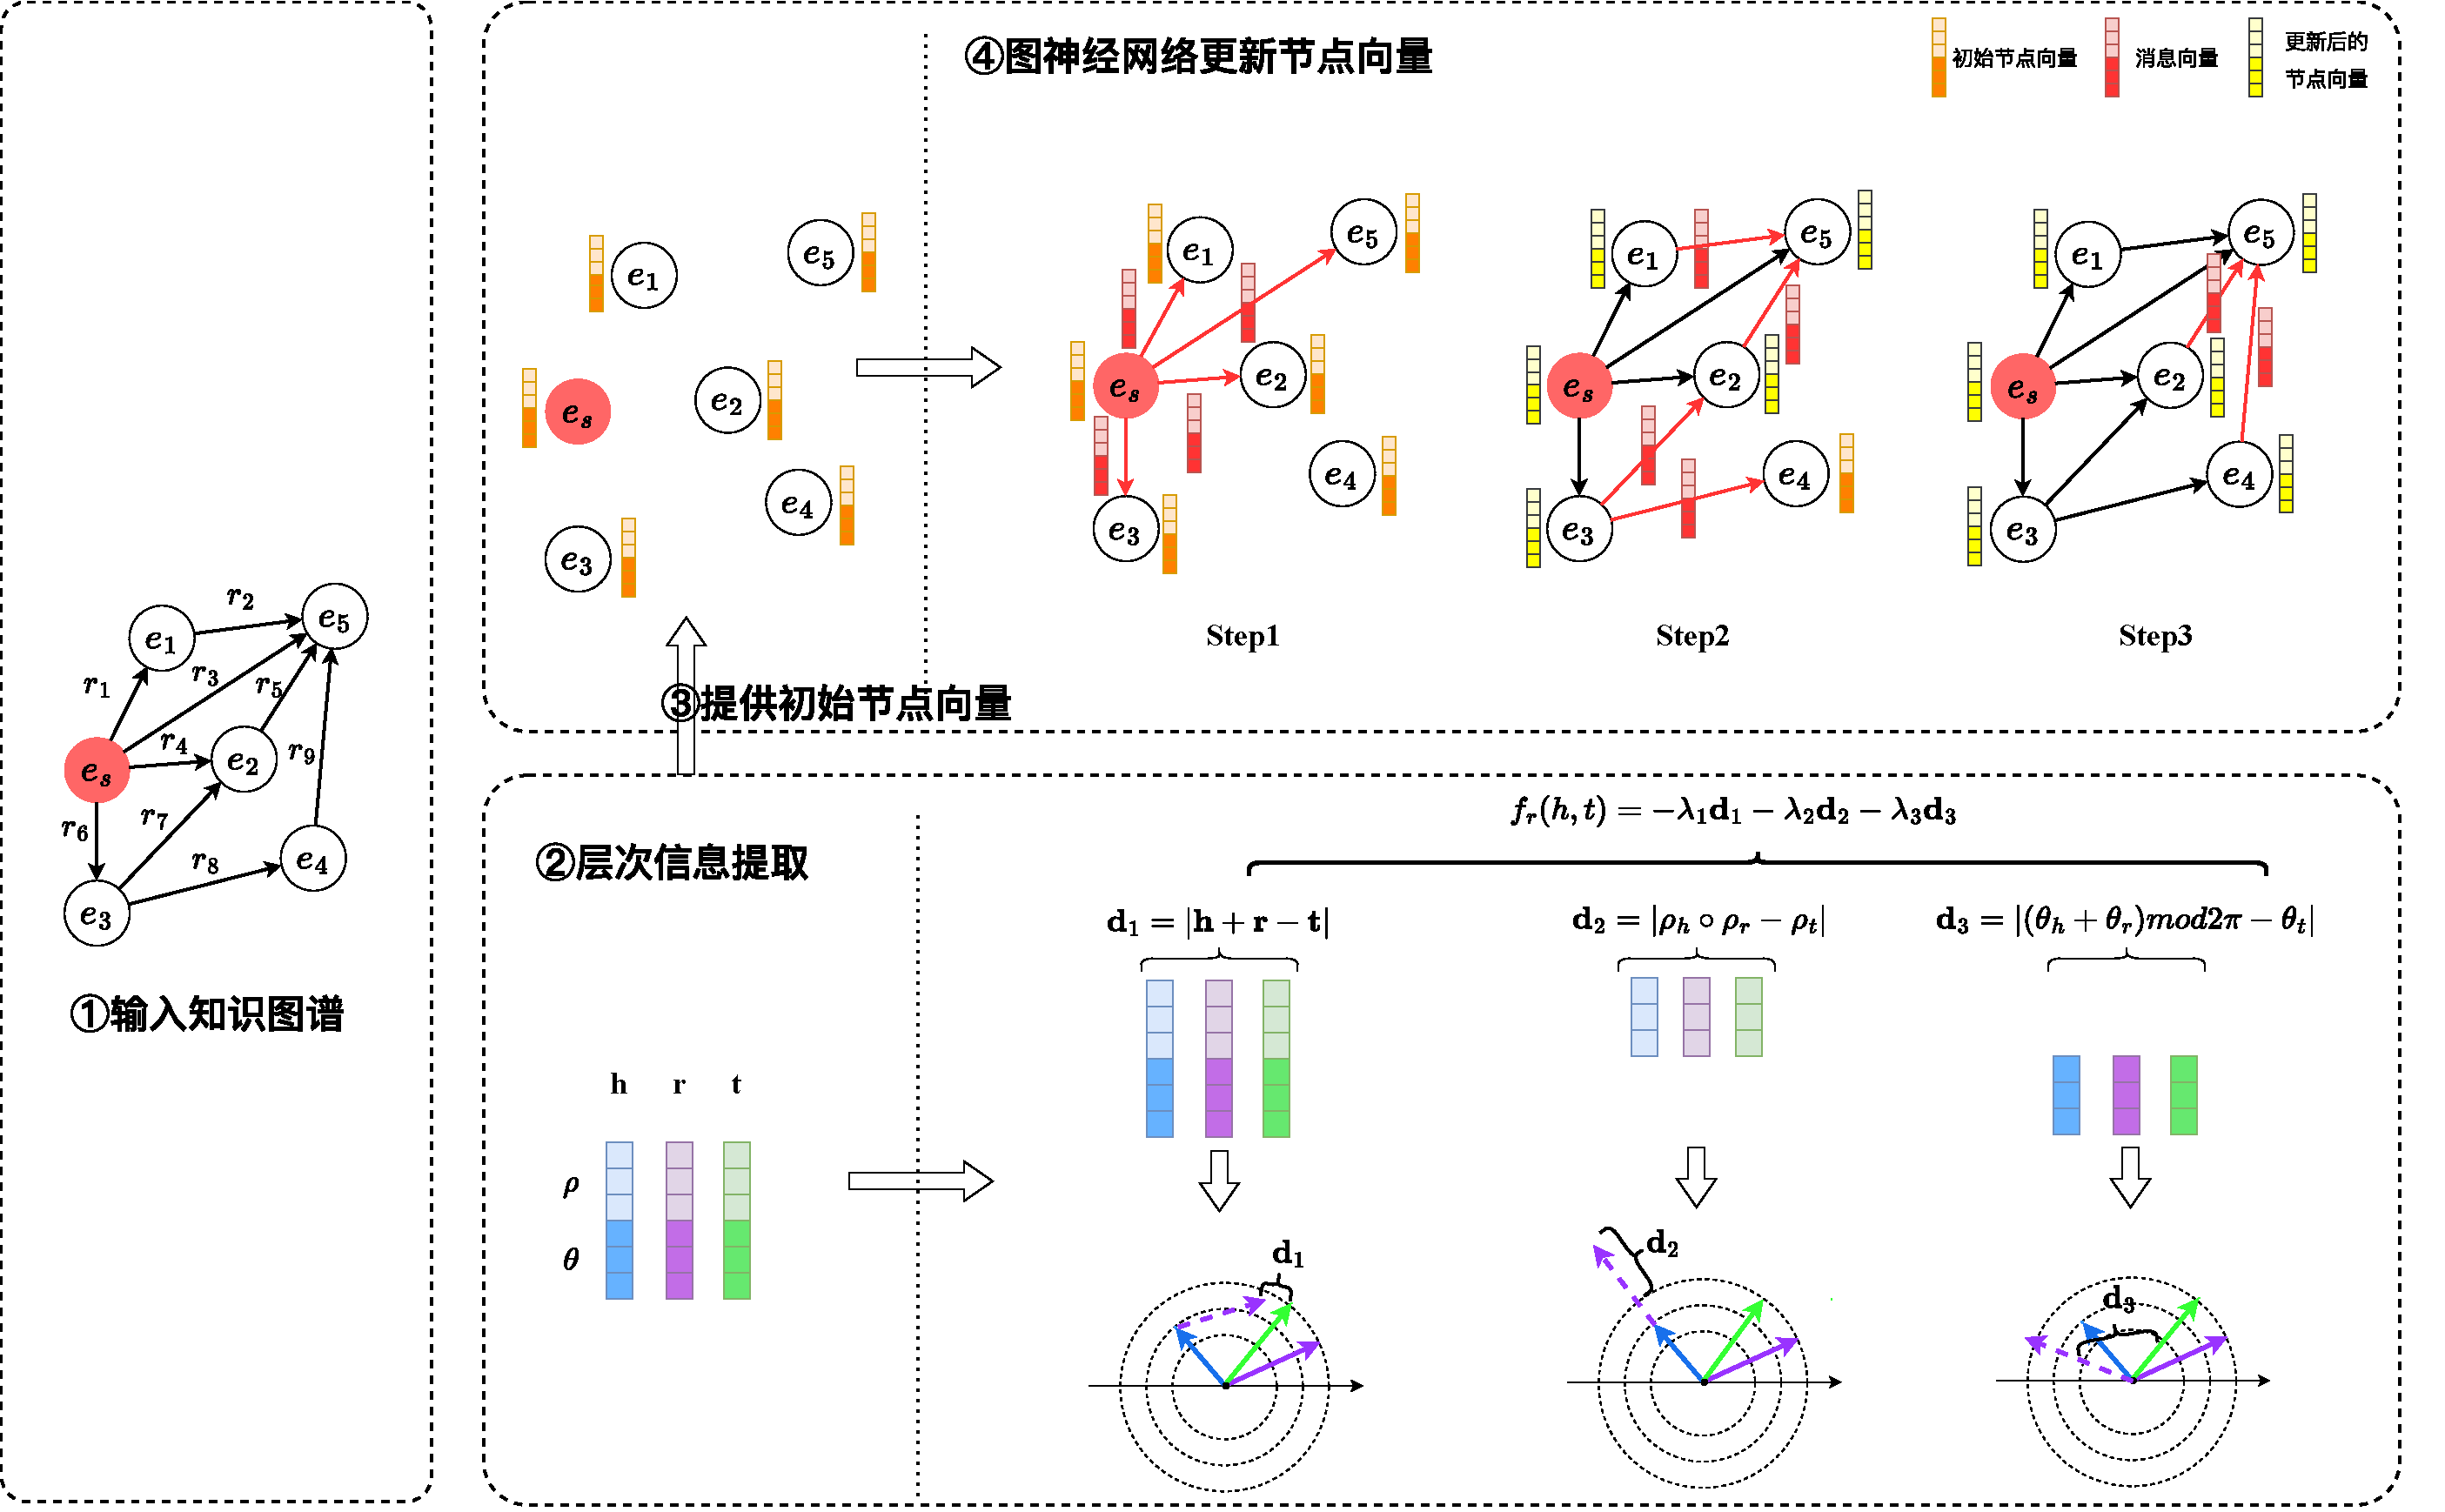
\includegraphics[width=0.4\textwidth]{2_Layers}
  \caption{层次信息提取模块结构图}
  \label{2_Layers}
\end{figure}

\subsection{极坐标系编码知识图谱}
层次信息提取模块可以通过极坐标系编码器将知识图谱中的知识编码为欧氏空间的表示向量,在结果中,每个实体和关系都对应着一个极坐标,可以表示为$(\bm{\rho}, \bm{\theta})$, 其中$\bm{\rho}$表示半径坐标向量,$\bm{\theta}$表示角坐标向量。半径坐标向量主要用于区分实体和关系的层次情况,而角坐标向量主要用于区分不同的实体和关系类型,从而保证了模块对知识图谱的表示能力。
在使用极坐标系编码器在欧氏空间上对知识图谱进行编码时,需要考虑如何设计得分函数的问题。本文采用翻译模型的思路,考虑将极坐标系下的欧氏距离度量函数融入评分函数中,以保证知识图谱学习过程的正确性。
对此,需要先分析如何通过计算得到极坐标系上的两点之间欧氏距离。
对极坐标系上的两点$p$和$q$,可以将两点表示成向量形式$\bm{p}$和$\bm{q}$,随后使用点积表示两点之间的欧氏距离,可以得到:
\begin{equation}
  \begin{aligned}
  \|\bm{p}-\bm{q}\|_2 & =\left((\bm{p}-\bm{q}) \cdot(\bm{p}-\bm{q})\right)^{\frac{1}{2}} \\
  & =\left(\|\bm{p}\|^2-2(\bm{p} \cdot \bm{q})+\|\bm{q}\|^2\right)^{\frac{1}{2}}
  \end{aligned}
\end{equation}
设$p$和$q$的极坐标分别为$(\bm{\rho_1}, \bm{\theta_1})$和$(\bm{\rho_2}, \bm{\theta_2})$,则两点之间的欧氏距离可以具体表示为:
\begin{equation}
  \|\bm{p}-\bm{q}\|_2=\left(\bm{\rho_1}^2-2 \bm{\rho_1} \bm{\rho_2} \cos \left(\bm{\theta_1}-\bm{\theta_2}\right)+\bm{\rho_2}^2\right)^{\frac{1}{2}}
  \label{equation_distance}
\end{equation}

通过应用公式\ref{equation_distance},可以采用翻译模型得分函数,实现知识三元组$(h, r, t)$的评分。

设$h, r, t$的极坐标分别是$\left(\bm{\rho_1}, \bm{\theta_1}\right)$,$\left(\bm{\rho_2}, \bm{\theta_2}\right)$和$\left(\bm{\rho_3}, \bm{\theta_3}\right)$,同时当$(h, r, t) \in F$时设它们的表示向量有$\|\bm{h} + \bm{r} - \bm{t}\|_2 = 0$,根据该假设可以得到极坐标系下欧氏距离的得分函数$f^E_r(h, t)$为:
\begin{equation}
  \begin{aligned}
    f^{E}_{r}\left(h, t\right) & =-\left\|\bm{h}+\bm{r}-\bm{t}\right\|_2 \\
    & =-(\bm{\rho_1}^2+\bm{\rho_2}^2+\bm{\rho_3}^2 + 2 \bm{\rho_1} \bm{\rho_2} \cos \left(\bm{\theta_1}-\bm{\theta_2}\right) \\
    & - 2 \bm{\rho_1} \bm{\rho_3} \cos \left(\bm{\theta_1}-\bm{\theta_3}\right) - 2 \bm{\rho_2} \bm{\rho_3} \cos \left(\bm{\theta_2}-\bm{\theta_3}\right))^{\frac{1}{2}}
  \end{aligned}
\end{equation}
该评分函数的思想是,将关系$r$视为极坐标系上的点$h$到$t$的变换,即有$\bm{h} + \bm{r} = \bm{t}$,目标是使得正例三元组的评分尽可能低,同时使负例三元组的得分尽量较高。

然而,仅使用基于距离的得分函数$f^E_r(h, t)$是不够的,如果将$p$和$q$的坐标转换成直角坐标,即$\bm{p}=\left(\bm{\rho_1} \cos \bm{\theta_1}, \bm{\rho_1} \sin \bm{\theta_1}\right), \bm{q}=\left(\bm{\rho_2} \cos \bm{\theta_2}, \bm{\rho_2} \sin \bm{\theta_2}\right)$,则两点之间的距离可以表示为:
\begin{equation}
  \begin{aligned}
  \|\bm{p}-\bm{q}\|_2 & =\left(\left(\bm{\rho_1} \cos \bm{\theta_1}-\bm{\rho_2} \cos \bm{\theta_2}\right)^2+\left(\bm{\rho_1} \sin \bm{\theta_1}-\bm{\rho_2} \sin \bm{\theta_2}\right)^2\right)^{\frac{1}{2}} \\
  % & =\sqrt{\bm{\rho_1}^2 \cos ^2 \bm{\theta_1}-2 \bm{\rho_1} \bm{\rho_2} \cos \bm{\theta_1} \cos \bm{\theta_2}+\bm{\rho_2}^2 \cos ^2 \bm{\theta_2}+\bm{\rho_1}^2 \sin ^2 \bm{\theta_1}-2 \bm{\rho_1} \bm{\rho_2} \sin \bm{\theta_1} \sin \bm{\theta_2}+\bm{\rho_2}^2 \sin ^2 \bm{\theta_2}} \\
  % & =\sqrt{\bm{\rho_1}^2\left(\cos ^2 \bm{\theta_1}+\sin ^2 \bm{\theta_1}\right)-2 \bm{\rho_1} \bm{\rho_2}\left(\cos \bm{\theta_1} \cos \bm{\theta_2}+\sin \bm{\theta_1} \sin \bm{\theta_2}\right)+\bm{\rho_2}^2\left(\cos ^2 \bm{\theta_2}+\sin ^2 \bm{\theta_2}\right)} \\
  & =\left(\bm{\rho_1}^2-2 \bm{\rho_1} \bm{\rho_2} \cos \left(\bm{\theta_1}-\bm{\theta_2}\right)+\bm{\rho_2}^2\right)^{\frac{1}{2}}
  \end{aligned}
\end{equation}
可以发现,极坐标系表示和直角坐标系表示在计算两点间的欧氏距离时是等价的。因此如果仅采用欧氏距离得分函数$f^E_r(h, t)$作为得分函数,则模型的得分函数将与TransE模型的得分函数相同,最终的训练效果也将一致。究其原因,是因为欧氏距离得分函数$f^E_r(h, t)$在实际训练过程中并没有具体区分半径坐标和角坐标,导致无法使用半径坐标来学习知识图谱中的层次结构信息,同时也没有使用角坐标来区分不同的实体和关系类别。对此,模块针对半径坐标和角坐标分别设计了两种得分函数,从而充分利用极坐标系的半径坐标和角坐标的优势进行知识图谱表示。

针对半径坐标,模块将$r$视为$h$到$t$的半径坐标缩放变化过程,即有$\bm{\rho_1} \circ \bm{\rho_2} = \bm{\rho_3}$,其中$\circ$为哈达玛积运算,即对向量$\bm{a}, \bm{b} \in \mathbb{R}^{d}$,有$\left(\mathbf{a} \circ \mathbf{b}\right)_i = \mathbf{a}_i \cdot \mathbf{b}_i$。
根据上述设定,可以得到半径坐标的得分函数$f^{\rho}_r(h, t)$为:
\begin{equation}
  f^{\rho}_r\left(h, t\right) =-\left\|\bm{\rho_1} \circ \bm{\rho_2} - \bm{\rho_3}\right\|_2
\end{equation}

针对角坐标,模块将$r$视为$h$到$t$的角坐标变换过程,即有$(\bm{\theta_1} + \bm{\theta_2}) \bmod 2 \pi = \bm{\theta_3}$。使用正弦函数进行变换,即可得到角坐标的得分函数$f^{\theta}_r(h, t)$为:
\begin{equation}
  f^{\theta}_r\left(h, t\right) =-\left\|\sin \left(\left(\bm{\theta_1}+\bm{\theta_2}-\bm{\theta_3}\right) / 2\right)\right\|_1
\end{equation}

最终模块整体的得分函数$f_r(h, t)$是对上述三个得分函数的加权求和,表示如下:
\begin{equation}
  \begin{aligned}
    f_r\left(h, t\right) &= -\lambda_1 f^{E}_r(h, t) -\lambda_2 f^{\rho}_r(h, t) -\lambda_3 f^{\theta}_r(h, t) \\
    &= -\lambda_1 \left\|\bm{h} + \bm{r} - \bm{t}\right\|_2 \\
    &-\lambda_2 \left\|\bm{\rho_1} \circ \bm{\rho_2} - \bm{\rho_3}\right\|_2 \\
    &-\lambda_3\left\|\sin \left(\left(\bm{\theta_1}+\bm{\theta_2}-\bm{\theta_3}\right) / 2\right)\right\|_1
  \end{aligned}
  \label{f_1}
\end{equation}
其中$\lambda_1$、$\lambda_2$和$\lambda_3$分别表示欧氏距离得分函数$f^E_r(h, t)$、半径坐标得分函数$f^{\rho}_r(h, t)$和角坐标得分函数$f^{\theta}_r(h, t)$的权重超参数。
通过上述得分函数训练模型,即可实现在保证模型学习正确性的情况下,利用半径坐标捕获知识图谱中的层次信息,同时利用角坐标区分不同的实体和关系类型,从而为其他模块提供数据支持。

在模型训练的过程中,采用自对抗负采样(Self-adversarial Negative Sampling)损失函数~\cite{sun2018rotate},可以表示为:
\begin{equation}
  \begin{aligned}
  L= & -\log \operatorname{Sigmoid}\left(\gamma-f_r(h, t)\right) \\
  & -\sum_{i=1}^n p\left(h_i, r_i, t_i\right) \log \operatorname{Sigmoid}(f_{r_i}(h_i, t_i))
  \end{aligned}
  \label{loss_1}
\end{equation}
其中$\gamma$是合页损失的固定边界值超参数,需要根据知识图谱进行手动调整。
同时,随机负例的采样概率$p(h_i, r_i, t_i)$可以表示为:
\begin{equation}
  p(h_i, r_i, t_i)=\frac{\exp f_{r_i}(h_i, t_i))}{\sum_j \exp f_{r_j}(h_j, t_j)}
  \label{abc}
\end{equation}

\subsection{半径坐标聚类}
使用极坐标系编码器完成知识图谱编码后,得到的表示向量主要包含两部分,分别是半径坐标向量和角坐标向量,其中的半径坐标向量包含了实体和关系的层次信息。
需要注意的是,半径坐标向量表达的层次信息是在连续空间上的,并且需要通过计算向量的模量来获取具体的层次,这导致半径坐标向量无法直接为后续模块提供清晰的层次信息。
为了方便后续模块直接获取实体和关系的层次信息,本节通过聚类算法将半径坐标向量转化为一系列离散的整数,作为实体和关系的层次级别。具体而言,模块采用K-Means聚类算法,对实体和关系的半径坐标向量进行聚类,从而将知识转换为K个层次。其中$K$为超参数,需要根据具体的知识图谱调整为不同的K值。具体过程如算法\ref{algorithm_kmeans}所示
完成聚类过程后即可得到知识图谱上所有实体和关系对应的的层次级别,范围是从0到$K-1$的连续整数值,可以为后续模块提供层次级别信息。
\begin{algorithm}[tb]
	\caption{层次信息提取K-Means模型训练算法}  
	\label{algorithm_kmeans}
	\begin{algorithmic}[1]
  \Require 半径坐标向量集合$D$, 聚类最大步数$\epsilon$
  \Ensure 半径坐标向量对应的层次级别集合$H$
  \State $\operatorname{Initiate}_{i=1, \cdots, K}(\bm{c_i})$ // 初始化聚类中心
  \State $n \leftarrow \operatorname{GetLength}(D)$ // 获取$D$的数据数量
  \Repeat 
  \For{$i \leftarrow 1$ to $n$}
  \State $\bm{\rho}_i \leftarrow \operatorname{GetItem}(D, i)$ // 获取$D$中的第$i$个向量
  \State $h_i \leftarrow \operatorname{argmin}_{j=1, \cdots, K} \|\bm{\rho}_i - \bm{c}_j\|^2$ // 选择最近的聚类中心作为层次标签
  \EndFor
  \Until{$t \geq \epsilon \mid t = \operatorname{NumberOfRepeat}()$} // 当聚类迭代步数超过最大聚类步数$\epsilon$时结束
  \State \Return $H = \{h_1, \cdots, h_n\}$
	\end{algorithmic}
\end{algorithm} 


\section{因果推断模块构建}
在训练图神经网络模型构建知识图谱表示学习模型的过程中,需要通过节点之间的消息传递机制实现神经节点张量的更新。然而各个节点的邻域结构可能存在差异。
图\ref{2_LocalStructure}显示了知识图谱NELL-995的两个节点的邻域子图,可以发现两个节点的邻域结构具有较大差异,在这种情况下使用相同的消息传递聚合方式会忽略这种邻域结构差异,从而降低知识图谱表示效果~\cite{chen2020measuring}。
换而言之,节点的邻域结构是一种重要的信息,在知识图谱表示过程中需要加以重视。
\begin{figure}
  \centering
  \subfloat[“太阳鱼”节点邻域子图]{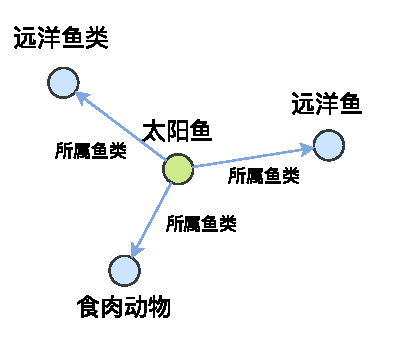
\includegraphics[width=0.3\textwidth]{2_LocalStructure_a}}
  \subfloat[“大比目鱼”节点邻域子图]{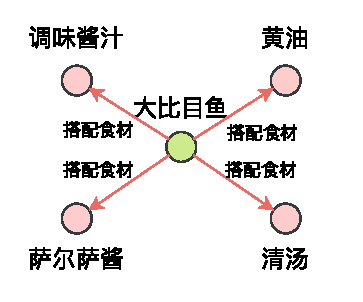
\includegraphics[width=0.3\textwidth]{2_LocalStructure_b}}
  \caption{知识图谱邻域结构差异}
  \label{2_LocalStructure}
\end{figure}
为了解决节点邻域结构差异问题,这就需要模型设计一个额外的模块来解决邻域结构差异的问题,例如采用注意力机制评估每个邻域节点的贡献。
然而训练图注意力机制难度较高,需要数据集提供大量标记数据,因此在对小规模数据集进行表示学习时就难以取得令人满意的效果~\cite{knyazev2019understanding}。
针对上述问题,本节提出了因果推断模块,该模块能够通过因果推断方式分析邻域结构差异,并根据神经节点的邻域信息决定是否接收来自邻域节点的消息,从而减少邻域结构差异对知识表示的影响。
同时,模块不采用深度学习模型而是采用SVM(Support Vector Machine,支持向量机)模型构建二元分类器,从而保证模块能够利用少量数据进行充分的模型训练。

\subsection{因果推断模块概览}
为了解决图神经网络模型中神经节点邻域结构差异问题,本文提出了一种新的方案,即采用因果推断机制评估邻域信息是否有助于节点进行知识表示,亦或会对节点的知识表示造成不利影响。完成分析后,模块能够提供邻域节点消息的取舍方案,从而降低邻域结构差异对知识表示的不利影响。
因果推断机制主要包括两个步骤,首先需要进行因果发现,随后需要通过因果干预获取因果效应。
因果发现过程是对各个变量之间的关系进行分析并得到因果图的过程。
因果干预则是通过随机实验调整因果图中的变量并比较因果干预前后的效果从而得到因果效应。

本节在介绍因果推断模块的过程中,首先介绍通过因果干预获取因果效应的过程,并指出了只有满足三种假设条件的情况下才能够通过因果推断获取因果效应。
随后在因果发现步骤中对图神经网络消息传递过程进行了分析,得到了相关变量并给出了图神经网络消息传递因果图,同时通过分析确认了模块符合三种假设条件,可以通过因果推断获取因果效应。
随后介绍模块的因果干预过程,即随机屏蔽来自特定邻域节点的消息并预测干预结果,通过对比原始结果和干预结果分析邻域局部结构对预测结果的因果效应,并决定是否接收来自特定邻域节点的消息。
最后介绍模块的具体实现方式,即综合考虑层次差异得分、决策差异得分、预测置信度得分和推理距离得分等多种因素,采用SVM模型构建二元分类器评估图神经网络节点是否接收来自特定邻域节点的消息。

\subsection{因果推断获取因果效应条件}
因果推断的目标是评估变量之间是否存在因果性,如果有,则分析变量间具体存在怎样的因果性,也就是因果效应。
以药品效果分析为例,设定药品数量为$X$,患者症状为$Y$,则现有机器学习的主流方法是学习$X$与$Y$之间的相关性,即探索在条件为$X$的情况下$Y$的情况是怎样的。
因果推断方法则更进一步,首先通过因果发现过程分析变量间的因果性并得到因果图,随后通过因果干预的方法随机地调整变量的值,获取因果干预后的结果并与现有事实进行比较,最终获取变量间的因果效应。
仍以药品效果分析为例,采用因果推断的方法对药品效果进行分析,则一种可行方案是:首先通过因果发现评估药品数量和患者症状间是否有因果性,这里我们认为两者存在因果性,并构建了如图\ref{2_CausalEffectMedicine}所示的因果图。
随后采用因果干预的方法,在安全剂量的范围内随机地调整药品数量并记录调整后得到的结果(患者症状),之后将调整后得到的结果与原有结果进行比较,并最终确定$X$与$Y$之间的因果效应。
\begin{figure}
  \centering
  
\includegraphics[width=0.3\textwidth]{2_CausalEffectMedicine}
  \caption{药品数量与患者症状因果图}
  \label{2_CausalEffectMedicine}
\end{figure}

因果效应常用的指标是ATE(Average Treatment Effect,平均因果效应),意义是计算受处理的和未受处理的群体效果差异的期望值。设$E(\cdot)$为期望值计算函数,$Y(W=k), k \in \{0, 1\}$为处理$W$为$k$时的结果,$k$可以为0或1,分别表示接收处理和不接受处理,则ATE可以表示为:
\begin{equation}
  ATE=\operatorname{E}\left(Y(W=1) - Y(W=0)\right)
  \label{equation_ATE}
\end{equation}
类似的,另一个指标是ITE(Individual Treatment Effect,个体因果效应),即计算单个受处理的和未受处理的个体效果差异的值。ITE可以表示为:
\begin{equation}
  ITE=Y(W=1) - Y(W=0)
  \label{equation_ITE}
\end{equation}

在前面药品效果分析样例中可以发现,随机试验在因果推断过程中具有重要作用。
这是由于因果推断的过程要求,同一个个体在相同条件下同时接受两种不同的处理,随后分析结果并进行比较才能得到因果效应。
在实际执行过程中可以发现,当个体接受了一种处理后,就发生了改变,无法满足同时接受不同处理的要求。
为了满足上述要求,一种可行的解决方案是:在满足以下三种假设条件的前提下,通过随机实验的方式开展实验并得到对应结果,随后将随机实验结果与原有结果进行比较,从而得到有效的因果效应~\cite{yao2021survey}。

\newtheorem{assumption}{Assumption}[section]
\begin{assumption}
  \textbf{稳定单位处理价值假设(Stable Unit Treatment Value Assumption):}
  任何个体的潜在结果$Y$(可以类比为治疗结果)不会因分配给其他单位的处理$W$(可以类比为治疗方式)而发生改变。对于每个个体,每次处理$W$都是相同的,同时会造成相同的结果$Y$。
  \label{1_Assumption}
\end{assumption}
上述假设强调了个体之间处理操作的独立性,以及对单一个体处理效果的一致性。

\begin{assumption}
  \textbf{可忽略性假设(Ignorability Assumption):}
  假设两个个体具有相同的背景变量$X$(可以类比为患者的性别、年龄、身高和体重等指标),则无论处理$W$分配的是什么,他们的潜在结果$Y$都是相同的。即处理分配与结果相互独立。使用$\perp$表示相互独立,则假设可以表示为:
  \begin{equation}
    W \perp Y(W=0), Y(W=1)) \mid X
  \end{equation}
  \label{2_Assumption}
\end{assumption}
上述假设具有两层含义:当两者的背景变量相同时,无论分配机制如何,他们的潜在结果都应该相同。另一方面,当两者的背景变量相同时,无论潜在结果值如何,他们的分配机制都应该相同。假设可以表示为:
\begin{equation}
  p\left(W \mid X=x, Y_i(0), Y_i(1)\right)=p\left(W \mid X=x, Y_j(0), Y_j(1)\right)
\end{equation}

\begin{assumption}
  \textbf{正向假设(Positivity Assumption):}
  对于任何背景变量$X$,处理$W$的分配概率$P$都不能是确定的。可以表示为:
  \begin{equation}
    P(W=w \mid X=x)>0, \quad \forall w \text { and } x
  \end{equation}
  \label{3_Assumption}
\end{assumption}
上述假设的目标是强调,所有的分配都是有可能而且随机的。如果出现分配概率确定的情况,例如老人$x$不能采用某种治疗方案$w$,则分配给该老人的治疗方案为$w$时会导致医疗事故,因此这种分配概率为零,即有$P(W=w \mid X=x) = 0$。
这种情况下无法实现随机性试验。可以注意到,在医学领域采用随机试验是有一定风险的,可能会产生医疗事故等一系列情况。但是在构建知识图谱表示学习模型的过程中则不会存在类似的风险。

当问题符合上述三种假设时,则有:
\begin{equation}
  \begin{aligned}
  \operatorname{E}[Y(W=w) \mid X=x] & =\operatorname{E}[Y(W=w) \mid W=w, X=x] \\
  & =\operatorname{E}\left[Y^F \mid W=w, X=x\right]
  \end{aligned}
  \label{equation_effect}
\end{equation}
其中$Y^F$表示观测结果的随机变量。公式\ref{equation_effect}即为符合上述假设时,因果效应可以通过观察随机实验的结果得到。
此时可以修改ATE的计算方法\ref{equation_ATE}。设个体总数为$Num$,则ATE可以修改为:
\begin{equation}
  \begin{aligned}
  ATE & =\operatorname{E}\left(\operatorname{E}\left(Y^F \mid W=1, X=x\right)-\operatorname{E}\left(Y^F \mid W=0, X=x\right)\right) \\
  & =\frac{1}{Num} \sum_i\left(Y_i(W=1)-Y_i(W=0)\right)
  \end{aligned}
  \label{equation_newATE}
\end{equation}
也就是说,可以通过对所有个体应用随机性因果干预实验,并通过对结果差值进行求均值可以得到ATE的计算结果,也就是因果效应。此时,ATE和ITE的关系可以表示为:
\begin{equation}
  ATE = \frac{1}{Num} \sum_i \mathrm{ITE}_i
  \label{equation_ATEandITE}
\end{equation}

综上所述,当因果推断过程满足上述三种假设时,采用因果干预获取的因果效应可以用于评估图神经网络模型的邻域信息是否存在邻域结构差异,并可以用于分析是否接收来自特定邻域节点的消息,从而能够提高模型的知识表示效果。

\subsection{因果发现}
因果发现过程主要是对变量进行分析,构建因果图。因果图是一种有向无环图,主要用于直观地描述变量间的因果关系。在因果图中,采用节点表示变量,并采用边表示变量间的因果关系。
为了构建因果图,首先需要分析图神经网络模型的内容。通过对图神经网络的分析发现,模型需要通过邻域实体间的消息传递,实现节点信息的更新。
根据图神经网络的消息传递过程,本文构建了如图\ref{2_CausalEffectView}所示的图神经网络消息传递因果图,在图中包含四种变量:
\begin{itemize}
  \item [1.] 初始中心节点信息变量$H_S$,该变量表示图神经网络模型中以某个节点作为子图结构中心,该节点对应的表示向量。变量的实例采用$\bm{h_s}$表示。
  \item [2.] 邻域节点信息变量$N$,该变量表示中心节点的邻域节点表示向量,能够通过信息传递更新中心节点信息。变量的个体实例采用$\bm{n_i}$表示,其中$\leq i \leq Num$,$Num$为邻域节点的数量,也就是说,中心节点有多少个邻域节点就有多少个变量实例。所有实例采用$\bm{n}$表示。
  \item [3.] 聚合消息变量$M$,该变量表示通过消息聚合函数,将初始节点传递过来的消息和邻域节点的表示向量进行聚合,得到的结果向量。变量的实例采用$\bm{m}$表示。
  \item [4.] 输出中心节点信息变量$H_O$,该变量表示子图结构中心节点,在完成消息传递和节点信息更新后得到的表示向量。变量的实例采用$\bm{h_o}$表示。
\end{itemize}

在图中可以发现,变量$H_S$和$N$都有一条指向$M$的有向边,表示$H_S$和$N$是影响模型聚合消息$M$的因素。$M$有一条指向$H_O$的有向边,原因是$M$是影响图神经网络模型更新节点信息得到$H_O$的因素,此外存在$H_S$指向$H_O$的有向边的原因是模型采用残差链接的方法,使得$H_S$能够直接影响$H_O$。
\begin{figure}
  \centering
  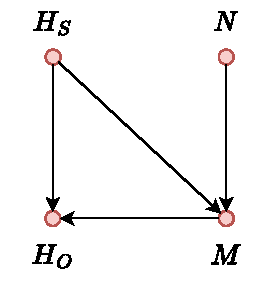
\includegraphics[width=0.2\textwidth]{2_CausalEffectView}
  \caption{图神经网络消息传递因果图}
  \label{2_CausalEffectView}
\end{figure}

针对因果分析得到的因果图和变量进行分析,评估它们是否符合三种假设条件。
首先,对于假设\ref{1_Assumption},可以选择任意两个不为邻域的节点(设置为不为邻域从而让两个节点作为相互独立的个体),并设置输出中心节点信息变量$H_O$为潜在结果$Y$,不接收来自特定邻域节点的消息$M$为处理$W$,则在同一时间对一个节点进行处理$W$并不会影响另一个节点的$Y$。同时针对一个节点执行$W$都会获得相同的$Y$,从而符合假设要求。
对于假设\ref{2_Assumption},可以选择任意两个不为邻域的节点,并设置初始中心节点信息变量$H_S$和邻域节点信息变量$N$为背景变量$X$,不接收来自特定邻域节点的消息$M$为处理$W$,则只要这两个节点的$X$和$W$相同,对应的$H_O$就会相同,从而符合假设要求。
对于假设\ref{3_Assumption},可以选择任意一个节点,并设置初始中心节点信息变量$H_S$和邻域节点信息变量$N$为背景变量$X$,不接收来自特定邻域节点的消息$M$为处理$W$,则该节点可以采用任何概率执行$W$而不会有任何问题,从而符合假设要求。
因此,根据上述分析可以得知,本节通过因果分析获取的因果图和变量满足三种假设条件,可以通过因果推断获取因果效应。

\subsection{因果干预}
在因果干预步骤中,目标是分析节点是否存在邻域结构差异的问题,并通过选择是否接收来自特定邻域节点的信息,从而降低邻域结构差异对模型的影响和提高知识图谱表示学习的效果。
\begin{figure}
  \centering
  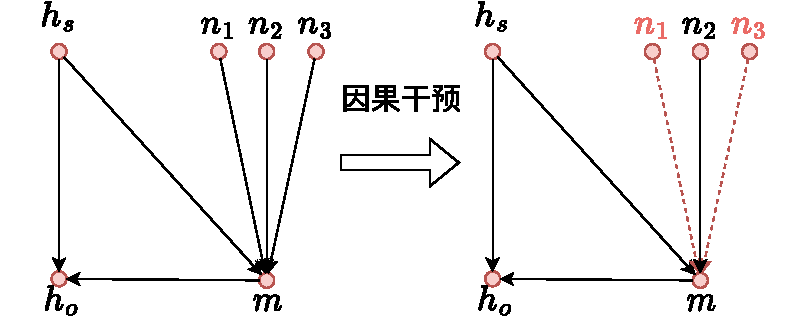
\includegraphics[width=0.55\textwidth]{2_CausalIntervention}
  \caption{图神经网络消息传递因果干预图}
  \label{2_CausalIntervention}
\end{figure}

在评估节点是否存在局部结构差异的过程中,主要采用因果干预的方法进行评估。如图\ref{2_CausalIntervention}所示,因果干预过程主要是针对各个邻域节点信息变量实例展开,通过选择屏蔽掉部分邻域节点到中心节点的消息传递,降低局部结构差异。令$\operatorname{rm}(\cdot)$表示屏蔽邻域节点到中心节点消息传递的函数,则通过调整邻域节点消息传递过程得到的因果效应,形式上可以采用ITE和ATE进行表示,分别为:
\begin{equation}
  \begin{aligned}
    ITE_i & =Y(W=1) - Y(W=0) \\
    & =Y(n_i)-Y_i(\operatorname{rm}(n_i))
  \end{aligned}
  \label{equation_CausalInterventionITE}
\end{equation}

\begin{equation}
  \begin{aligned}
    ATE & =\operatorname{E}\left(\operatorname{E}\left(Y^F \mid W=1, X=x\right)-\operatorname{E}\left(Y^F \mid W=0, X=x\right)\right) \\
    & =\frac{1}{N} \sum_i\left(Y_i(n_i)-Y_i(\operatorname{rm}(n_i))\right)
  \end{aligned}
  \label{equation_CausalInterventionATE}
\end{equation}

为了确定哪些邻域节点消息在消息传递过程中需要屏蔽,本文设计了一种二元分类器,能够根据邻域子图和节点的属性确定是否屏蔽来自邻域节点的信息。该分类器的输入主要包括以下内容:层次差异得分、决策差异得分、预测置信度得分和推理距离得分。

\textbf{层次差异得分}是计算中心节点和邻域节点的层次级别的差值。在通常情况下,知识三元组的头尾实体所处的层次级别差异度都相对较小,因此可以考虑将层次差异得分纳入分类器中,通过分析各个邻域节点是否与中心节点的层次级别相差较小来评估是否接收来自邻域节点的信息。设中心节点的层次级别为$h_c$,邻域节点的层次级别为$h_n$,则层次差异得分$v_h$的计算方式为:
\begin{equation}
  v_h = h_c - h_n
  \label{get1}
\end{equation}

\textbf{决策差异得分}为是否接收随机数量的邻域节点信息对模型预测结果的方差。如果得到的方差较大,则说明对邻域节点消息的轻微改变会导致预测结果发生重大变化,这意味着节点的邻域结构存在较大差异,应该通过屏蔽邻域节点消息来降低邻域结构差异带来的影响。令$\operatorname{var}(\cdot)$为方差计算函数,$K$为随机屏蔽若干邻域节点消息的实验次数,$n_k$为第$k$次实验时保留消息的邻域节点集合,则决策差异得分$v_d$的计算方式为:
\begin{equation}
  v_d = \operatorname{var}(Y(X=x, N=n_k) \mid k \in K)
  \label{get2}
\end{equation}
需要注意的是,由于决策差异得分的计算过程是采用所有中心节点的邻域节点进行评估,所以参与计算的邻域节点都共享相同的决策差异得分。

\textbf{预测置信度得分}是计算接收和不接收邻域节点信息得到的正确答案置信度的差值。一般认为,置信度体现了模型对预测结果的确信程度,高置信度代表模型倾向于该答案,因此通过比较正确节点置信度的高低并计算差值,可以评估接收邻域节点信息是否有益于模型做出决策。设不接收来自邻域的消息的置信度为$p_c$,接收来自邻域的消息的置信度为$p_n$,则预测置信度得分$v_c$的计算方式为:
\begin{equation}
  v_c = p_c - p_n
  \label{get3}
\end{equation}

\textbf{推理距离得分}是评估邻域节点距离初始查询节点$e_q$的距离。考虑到一般情况下实体间的距离越近则信息传递越强,计算当前节点到初始查询节点的距离得分有助于帮助模型选择相对较短的推理路径。设中心节点和邻域节点距离初始查询节点的距离分别为$l_c$和$l_n$,则推理距离得分$v_l$的计算方式为:
\begin{equation}
  v_l = l_c - l_n
  \label{get4}
\end{equation}
考虑到知识图谱中两点之间可能有多条查询路径和对应的距离,为了简化计算,此处的距离计算方式是从完整知识图谱中提取的邻域子图中两点间最短的查询路径的距离。

对上述输入内容进行分析,可以发现输入内容中的决策差异得分计算过程与ATE的计算方法\ref{equation_newATE}类似,同时其他输入内容与ITE的计算公式\ref{equation_ITE}相同,因此对上述输入内容进行分析等同于分析模型进行随机化因果干预后得到的因果效应,有助于提高模型的稳定性和合理性。
为了降低二元分类器的复杂性,保证模型能够在知识图谱数据量较少的情况下进行学习和训练,本文选择使用SVM模型训练二元分类器,用于评估是否进行因果干预。
设置一个阈值$T$表示SVM进行二元分类的阈值,高于该阈值则选择因果干预后的结果$\bm{\hat{h}}_o$,否则则选择保留邻域信息的知识图谱表示结果$\bm{h}_o$。模型决策过程可以表示如下:
\begin{equation}
  \bm{h}_o = \left\{\begin{array}{l}
  \bm{h}_o,\quad p < T, \\
  \bm{\hat{h}}_o,\quad p \geq T,
  \end{array} \quad p = \operatorname{SVM}\left(v_h, v_d, v_c, v_l\right)\right.
  \label{equation_SVM}
\end{equation}

为了训练SVM二元分类器,首先需要进行因果干预数据集$D$的构建。构建数据集的过程可以表示为:
\begin{equation}
  D = \{((v_h, v_d, v_c, v_l), f) \mid (h, r, t) \in F \cup (h, r, t) \notin F\},\quad f = \operatorname{model}(\bm{\hat{h}}_o)
\end{equation}
其中$\operatorname{model}$表示应用知识图谱表示学习模型进行知识图谱问答实验得到的结果,当正确结果排名在前$K$名时则返回1,否则返回-1。这里我们将$K$设置为10,从而对应知识图谱补全任务的Hits@10指标。
这里利用$\operatorname{model}$计算得到的$f$值的作用是评估加入因果干预后是否会帮助模型获取正确的实验结果,从而提高模型表示效果。
在具体构建数据集时,通过随机地将事实三元组中的实体和关系替换为其他实体和关系,得到候选三元组集合,其中的三元组$(h, r, t)$可以是事实三元组,也可以是潜在事实三元组。
随后对每个三元组$t$计算知识图谱表示结果$\bm{h}_o$,通过因果干预得到$\bm{\hat{h}}_o$并计算对应的$f$,同时针对因果干预前后的结果计算$v_h, v_d, v_c, v_l$。通过上述过程即可实现数据集$D$的构建。
可以发现,对同一个邻域可以通过因果干预的方式构建多个训练数据,从而能够利用少量数据构建大量数据集并实现模型训练。
完成数据集构建后,即可对模型进行训练。训练模型的过程如算法\ref{algorithm_SVM}所示。
\begin{algorithm}[tb]
	\caption{因果推断支持向量机二分类模型训练算法}
	\label{algorithm_SVM}
	\begin{algorithmic}[1]
    \Require 数据集$D$, 学习率$\alpha$, 停止阈值$\epsilon$
    \Ensure 模型参数$\bm{w}$和$\bm{b}$
    \State $\bm{w} \leftarrow \bm{0},\quad \bm{b} \leftarrow \bm{0}$ // 模型参数初始化
    \For{$((v_h, v_d, v_c, v_l)_i, f_i) \in D$}
    \State $t_i \leftarrow f_i (\bm{w} (v_h, v_d, v_c, v_l)_i + \bm{b})$ // 计算函数间隔
    \State $L(\bm{w}, \bm{b}) \leftarrow \frac{1}{2} \|\bm{w}\|^2 + \sum_{i=1}^{n} \max(0, 1 - t_i)$ // 构建损失函数
    \EndFor
    \Repeat
    \State $((v_h, v_d, v_c, v_l)_i, f_i) \leftarrow \operatorname{Sample}(D)$ // 随机采样
    \If{$t_i < 1$}
    \State $\nabla_{\bm{w}} L(\bm{w}, \bm{b}) \leftarrow \bm{w} - f_i (v_h, v_d, v_c, v_l)_i$ // 计算$\bm{w}$梯度
    \State $\nabla_{\bm{b}} L(\bm{w}, \bm{b}) \leftarrow - f_i$ // 计算$\bm{b}$梯度
    \State $\bm{w} \leftarrow \bm{w} - \alpha \nabla_{\bm{w}},\quad \bm{b} \leftarrow \bm{b} - \alpha \nabla_{\bm{b}}$ // 更新参数
    \State $t_i \leftarrow f_i (\bm{w} (v_h, v_d, v_c, v_l)_i + \bm{b})$ // 更新函数间隔
    \State $L(\bm{w}, \bm{b}) \leftarrow \frac{1}{2} \|\bm{w}\|^2 + \sum_{i=1}^{n} \max(0, 1 - t_i)$ // 更新损失函数
    \EndIf
    \Until{$L(\bm{w}, \bm{b}) < \epsilon$}
    \State \Return $\bm{w}, \bm{b}$
	\end{algorithmic}
\end{algorithm} 


\section{图神经网络模块构建}
% 图神经网络模块采用图神经网络模型,构建的图神经网络模型能够充分利用知识图谱中各个实体的邻域结构信息,并通过知识邻域间的信息传递进行数据更新。在此过程中,模块利用层次信息提取模块的层次信息作为辅助,采用因果推断模块评估是否接收邻域信息。完成训练后的模型,能够将输入的知识结构化三元组转换为表示向量,并可以用于后续知识推理工作。
本章构建的知识图谱表示学习模型主要采用图神经网络模型,能够结合前文所述的层次信息提取模块和因果推断模块进行知识图谱表示。
在具体应用过程中,首先需要使用层次信息提取模块获取知识三元组的初始表示向量和层次信息,并将这些内容作为输入提供给图神经网络模块。
随后进行图神经网络模型训练,训练过程中利用因果推断模块分析当前神经节点是否存在邻域结构差异问题,并评估是否接收来自邻域节点的信息进行节点信息更新。
完成训练后的图神经网络模型能够捕获知识图谱的邻域结构信息,实现高质量的知识表示。

在图神经网络模块的介绍过程中,本节首先进行图神经网络模块概览,介绍模块的主要内容并给出模块结构图。
随后介绍图神经网络构建过程,重点介绍模型如何构建关系有向图并捕获知识图谱邻域信息。
最后介绍图神经网络模型的消息传递机制,该部分实现了对层次信息提取模块和因果推断模块的结合,通过层次信息提取模块获取知识的初始向量,并将层次信息等内容作为输入提供给因果推断模块,评估是否接收邻域节点信息,实现消息传递。

\subsection{图神经网络模块概览}
在本章第三节介绍的层次信息提取模块将捕获知识图谱层次结构信息方面作为重要目标。然而,该模块在进行知识表示时缺少对邻域信息的分析和评估,限制了模型的效果。
为了保证模型在关注层次信息和因果信息的同时提高对邻域信息的利用能力,本节设计了一种融合层次信息和因果信息的图神经网络模块。
模块首先将层次信息提取模块得到的实体表示向量作为各个节点的初始表示,同时将各个实体的层次级别作为因果推断模块的输入,参与消息传递过程。
为了获取知识图谱邻域信息,模块首先针对每个实体构建相应的知识图谱子图,随后通过消息传递的方式传递邻域信息,实现节点信息更新。
通过上述途径保证了模型能够利用知识图谱的层次结构信息、消息传递过程中的因果信息以及知识图谱邻域信息,提高知识图谱表示效果。

\begin{figure}
  \centering
  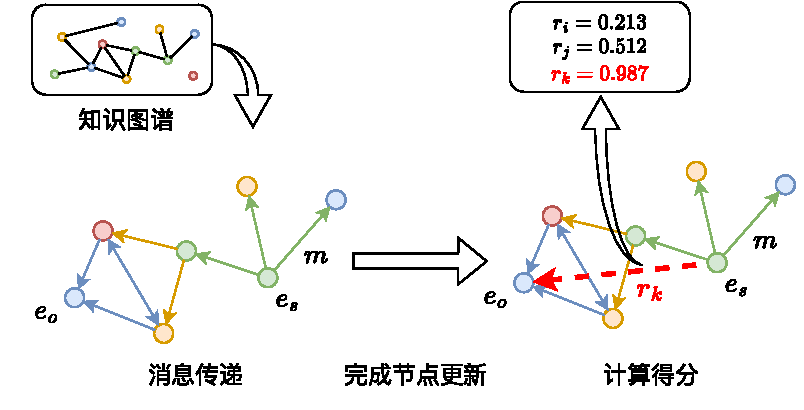
\includegraphics[width=0.7\textwidth]{2_GNN}
  \caption{图神经网络模块结构图}
  \label{2_GNN}
\end{figure}
本节构建的图神经网络模块如图\ref{2_GNN}所示,在模块构建的过程中,主要包含以下步骤:
首先需要进行邻域子图构建,通过同时从知识三元组的头实体$h$和尾实体$t$开始迭代地获取关联实体,并统计头尾之间长度不超过最大长度$L$的节点的交集,作为邻域子图。
除了这种邻域子图构建方法之外,本节还研究了一种基于动态规划的邻域子图构建方法,这种方法具有更好的适用性,能解决更复杂的知识图谱补全问题。
随后进行消息传递,消息传递过程首先利用层次信息提取模块得到的实体和关系向量作为初始的节点信息,随后通过消息聚合函数将邻域子图中其他节点的信息聚合起来,并通过信息更新函数将新获取到的消息与当前节点的原有信息结合,实现节点信息更新。
在消息传递的过程中,对于是否接收特定邻域节点的信息需要利用因果推断模块进行评估。
完成模型训练后得到的图神经网络模型可以将知识信息转换成表示向量,并能够应用于知识图谱补全和知识图谱问答等下游任务中。

\subsection{邻域子图构建}
在利用图神经网络模型进行知识图谱表示时,由于邻域信息对知识表示具有重要作用,因此本文构建的图神经网络模块首先会通过递归的方式进行知识图谱子图构建。
常用的构建邻域子图的方法是:对每组知识三元组,选择其对应知识图谱中的头尾实体作为起始节点,依次向外获取邻域节点直到达到最大距离$L$,并对获取到的邻域节点取交集从而完成邻域子图构建~\cite{teru2020inductive}。
具体过程如算法\ref{algorithm_normal}所示。可以发现这种算法的时间复杂度较高,同时在并行处理大规模知识数据时对系统内存需求量较大,尤其不利于处理每个节点都带有大量关联节点的大规模知识图谱。
该算法的另一个问题是需要同时知道头实体和尾实体才能够进行邻域子图构建,即该算法只能用于解决$(h, ?, t)$类型的知识图谱补全问题,而难以直接用来解决只提供一个实体的知识图谱补全问题,如$(h, r, ?)$和$(?, r, t)$,限制了模型的应用。
\begin{algorithm}[tb]
	\caption{邻域子图构建常规算法}  
	\label{algorithm_normal}
	\begin{algorithmic}[1]
  \Require 知识图谱事实集合$F$, 头实体$h$, 尾实体$t$, 最大距离$L$
  \Ensure 知识图谱邻域子图$G_{neighbor}$
  \State $F_{h}^{0} \leftarrow \varnothing, F_{t}^{0} \leftarrow \varnothing$ // 初始化邻域知识集合
  \State $E_{h}^{0} \leftarrow \{h\}, E_{t}^{0} \leftarrow \{t\}$ // 初始化邻域实体集合
  \For{$i \leftarrow 1$ to $L$}
  \State $F_{h}^{i} \leftarrow \{(h_i, r_i, t_i) \in F \mid h_i \in E_{h}^{i-1}\}$ // 获取第$i$层头实体邻域知识
  \State $E_{h}^{i} \leftarrow \{t_i \mid (h_i, r_i, t_i) \in F_{h}^{i}\}$ // 获取第$i$层头实体邻域实体
  \State $F_{t}^{i} \leftarrow \{(h_i, r_i, t_i) \in F \mid t_i \in E_{t}^{i-1}\}$ // 获取第$i$层尾实体邻域知识
  \State $E_{t}^{i} \leftarrow \{h_i \mid (h_i, r_i, t_i) \in F_{t}^{i}\}$ // 获取第$i$层尾实体邻域实体
  \EndFor
  \For{$i \leftarrow 0$ to $L$}
  \State $F_{int}^{i} \leftarrow F_{h}^{i} \cap F_{t}^{L-i}$ // 获取邻域知识交集
  % \State $E_{int}^{i} \leftarrow \{E_{h}^{i} \cap E_{t}^{L-i}\}$ // 获取邻域实体交集
  \EndFor
  % \State $G_{neighbor} \leftarrow \{E_{int}, R_{int}\}$ // 获取邻域子图
  \State $G_{neighbor} \leftarrow F_{int}$ // 获取知识图谱邻域子图
  \State \Return $G_{neighbor}$
	\end{algorithmic}
\end{algorithm} 

本文采用了简化的邻域子图构建方法,能够取得与算法\ref{algorithm_normal}相同的效果。具体过程如算法\ref{algorithm_simple}所示。
算法首先以知识三元组中的一个实体作为起点,随后采用递归的方式从最新的一层向外扩展节点,并在扩展节点的同时进行消息传递,直到扩展达到到最大距离$L$,此时所有起点到终点的路径长度均为最大距离$L$。
可以发现以这种方式构建的邻域子图不需要与知识三元组中另一个实体的邻域子图取交集,因此构建的子图不小于算法\ref{algorithm_normal}构建的子图。
为了避免保存知识图谱邻域子图对系统内存造成的压力,本文选择让算法可以在每次向外扩展节点时进行消息传递,从而不再需要在完成整个知识图谱邻域子图构建后再进行消息传递。
这一方法使得系统不需要保存知识图谱邻域子图,显著降低了对系统内存的要求,并使得模型能够处理具有大量关联节点的大规模知识图谱。
此外该算法能够解决仅提供单一实体的知识图谱补全问题,具有更好的适用性。完整的算法包含消息传递过程,如算法\ref{algorithm_GNN}所示。
\begin{algorithm}[tb]
	\caption{邻域子图构建简化算法}
	\label{algorithm_simple}
	\begin{algorithmic}[1]
  \Require 知识图谱事实集合$F$, 实体$e$, 最大距离$L$
  \Ensure 知识图谱邻域子图$G_{neighbor}$
  \State $F_{e}^{0} \leftarrow \varnothing$ // 初始化邻域知识集合
  \State $E_{e}^{0} \leftarrow \{e\}$ // 初始化邻域实体集合
  \For{$i \leftarrow 1$ to $L$}
  \State $F_{e}^{i} \leftarrow \{(h_i, r_i, t_i) \in F \mid h_i \in E_{e}^{i-1}\}$ // 获取第$i$层邻域知识
  \State $E_{e}^{i} \leftarrow \{t_i \mid (h_i, r_i, t_i) \in F_{e}^{i}\}$ // 获取第$i$层邻域实体
  \EndFor
  \State $G_{neighbor} \leftarrow F_{e}$ // 获取知识图谱邻域子图
  \State \Return $G_{neighbor}$
	\end{algorithmic}
\end{algorithm} 

\subsection{消息传递}
在进行邻域子图构建后,模块需要利用图神经网络模型对给定的知识三元组进行知识表示,这时需要通过消息传递机制进行节点邻域信息的获取和节点信息的更新。
消息传递过程主要包括两步:首先进行消息聚合获取邻域子图中所有节点的节点信息(包括节点自身的信息),并通过聚合函数进行聚合。消息聚合可以表示为:
\begin{equation}
  \bm{m} = \operatorname{AGGREGATE}(\bm{h_s}, \bm{n})
\end{equation}
随后进行节点信息更新,通过使用更新函数将来自邻域的消息和节点自身信息结合起来进行更新,实现节点信息的更新。节点信息更新可以表示为:
\begin{equation}
  \bm{h_o} = \operatorname{UPDATE}(\bm{h_s}, \bm{m})
\end{equation}
上述两步也可以合并到一起,得到的消息传递函数可以表示为:
\begin{equation}
  \bm{h_o} = \operatorname{UPDATE}(\bm{h_s}, \operatorname{AGGREGATE}(\bm{h_s}, \bm{n}))
  \label{equation_MessagePassing}
\end{equation}
因此,在构建消息传递函数的过程中,主要需要考虑如何设计消息聚合部分和节点信息更新部分的内容。
考虑到给定不同的知识三元组,得到的邻域子图可能相同,但用于推理的证据通常情况下是不同的。因此,为了从邻域子图中获取与给定的知识三元组相关的知识并提高搜集邻域知识过程的可解释性,模块在消息聚合部分使用注意力机制以评估不同邻域知识的重要性,并采用一个GRU层作为门控机制,减少GNN模型的限制并维护信息的长期传播。消息传递函数可以表示为:
\begin{equation}
  \bm{h_o} = \operatorname{GRU}(\mathbf{W} \cdot \sum_{\bm{n_i} \in \bm{n}}{\bm{\alpha} \cdot (\bm{h_s} + \bm{n_i})})
  % \bm{h_o}^{k}=\delta\left(\mathbf{W}^{\ell} \cdot \sum_{\left(e_s, r, e_o\right) \in \hat{\mathcal{E}}_{e q}^{\ell}} \alpha_{e_s, r, e_o \mid r_q}^{\ell}\left(\boldsymbol{h}_{e_s}^{\ell-1}\left(e_q, r_q\right)+\boldsymbol{h}_r^{\ell}\right)\right)
  \label{equation_newMessagePassing}
\end{equation}
其中的注意力权重$\bm{\alpha}$可以表示为:
\begin{equation}
  \bm{\alpha} = \operatorname{Sigmoid}(\mathbf{W_{1}} \cdot \operatorname{ReLU}(\mathbf{W_{2}} \cdot (\bm{h_s} + \bm{n_i} + \bm{h}_q)))
  % \alpha_{e_s, r, e_o \mid r_q}^{\ell}=\sigma\left(\left(\boldsymbol{w}_\alpha^{\ell}\right)^{\top} \operatorname{ReLU}\left(\boldsymbol{W}_\alpha^{\ell} \cdot\left(\boldsymbol{h}_{e_s}^{\ell-1}\left(e_q, r_q\right) \oplus \boldsymbol{h}_r^{\ell} \oplus \boldsymbol{h}_{r_q}^{\ell}\right)\right)\right)
  \label{equation_Alpha}
\end{equation}
其中,$\bm{h}_q$是查询问题的关系对应的表示向量。
同时,可以在消息聚合部分融入因果推断模块的二元分类器,用于分析节点邻域是否存在局部性差异,并决定是否接收邻域节点信息。通过随机屏蔽掉一定的邻域消息,并计算对应的得分$v_h, v_d, v_c, v_l$和因果干预向量$\bm{\hat{h_o}}$,随后使用二元分类器计算因果干预后得分$p$,如果高于阈值$T$则选择因果干预后的结果$\bm{\hat{h_o}}$,否则仍然选择保留邻域信息的结果$\bm{h_o}$。这一过程可以表示为:
\begin{equation}
  \bm{h_o} = \left\{\begin{array}{l}
  \bm{h_o},\quad p < T, \\
  \bm{\hat{h_o}},\quad p \geq T,
  \end{array} \quad p = \operatorname{SVM}\left(v_h, v_d, v_c, v_l\right)\right.
  \label{equation_finalMessagePassing}
\end{equation}

在通过消息传递机制完成了节点信息更新后,各个节点完成了消息传递和更新,节点的表示向量中也融入了层次结构信息和邻域信息。
随后为了模块进行知识表示,需要选择适合的得分函数。考虑到表示向量$\bm{h_o}$包含了最大递归遍历距离为$L$的邻域子图内的信息,因此构建的得分函数采用了一个线性层进行计算最终得分。这里让$\bm{h_o}$表示知识三元组$(h, r, ?)$、$(h, ?, t)$或$(?, r, t)$中缺失信息的表示向量,则得分函数可以表示为:
\begin{equation}
  f_{r}(h, t) = \mathbf{W} \cdot \bm{h_o}
  % \operatorname{score}\left(u, r_t, v\right)=\mathbf{W}^T\left[\mathbf{h}_{\mathcal{G}_{\left(u, v, r_t\right)}^L}^L \oplus \mathbf{h}_u^L \oplus \mathbf{h}_v^L \oplus \mathbf{e}_{r_t}\right]
  \label{equation_GNNScore}
\end{equation}
模块可以使用得分函数计算目标知识三元组的得分,并根据得分排名选择缺失信息对应的实体或关系。

模型训练过程采用的损失函数与层次信息提取模块的损失函数\ref{loss_1}相同,同样为自对抗负采样(Self-adversarial Negative Sampling)损失函数,可以表示为:
\begin{equation}
  \begin{aligned}
  L= & -\log \operatorname{Sigmoid}\left(\gamma-f_r(h, t)\right) \\
  & -\sum_{i=1}^n p\left(h_i, r_i, t_i\right) \log \operatorname{Sigmoid}(f_{r_i}(h_i, t_i))
  \end{aligned}
\end{equation}
其中$\gamma$是合页损失的固定边界值超参数,需要根据知识图谱进行手动调整。
同时,随机负例的采样概率$p(h_i, r_i, t_i)$可以表示为:
\begin{equation}
  p(h_i, r_i, t_i)=\frac{\exp f_{r_i}(h_i, t_i))}{\sum_j \exp f_{r_j}(h_j, t_j)}
\end{equation}

至此,完成了对知识图谱表示学习模型NORMAN的图神经网络模块的全部介绍。
整个图神经网络模块的具体使用过程如算法\ref{algorithm_GNN}所示。可以发现图神经网络模块融合了层次信息提取模块和因果推断模块的内容,能够将知识信息转换为知识表示向量。
在图神经网络模块中融合了层次信息提取模块和因果推断模块的内容,实现了在知识图谱表示过程中维护知识图谱内的层次信息、因果信息和邻域信息,为知识图谱补全等下游任务提供支持。
% 算法(需要包含三个模块的内容。首先层次信息提取模块获取层次级别和初始向量,随后图神经网络模块边构建邻域子图边消息传递,消息传递的过程中利用了层次信息提取模块的层次级别和因果推断模块的二元分类器。最后通过图神经网络模块的评分函数,可以给出知识三元组的得分,完成知识图谱表示学习模型。利用模型可以解决知识图谱补全等下游任务。)
\begin{algorithm}[H]
	\caption{图神经网络模型算法}  
	\label{algorithm_GNN}
	\begin{algorithmic}[1]
  \Require 知识图谱事实集合$F$, 知识三元组$(h, r, t)$, 最大距离$L$
  \Ensure 知识表示向量$(\bm{h}, \bm{r}, \bm{t})$
  \State $(F_H, E_H, R_H) \leftarrow \operatorname{GetHierarchy}(F)$ // 通过层次信息提取模块,获取初始知识表示向量集合、实体层次集合和关系层次集合
  \For{$e \in \{h, r, t\}$}
  \State $F_{e}^{0} \leftarrow \varnothing$ // 初始化邻域知识集合
  \State $E_{e}^{0} \leftarrow \{e\}$ // 初始化邻域实体集合
  \For{$i \leftarrow 1$ to $L$}
  \State $F_{e}^{i} \leftarrow \{(h_i, r_i, t_i) \in F \mid h_i \in E_{e}^{i-1}\}$ // 获取第$i$层邻域知识
  \State $E_{e}^{i} \leftarrow \{t_i \mid (h_i, r_i, t_i) \in F_{e}^{i}\}$ // 获取第$i$层邻域实体
  \State $\bm{e_o} \leftarrow \operatorname{MessagePassing}(E_{e}^{i}, F_H)$ // 通过公式\ref{equation_newMessagePassing}进行消息传递
  \For{$n \in E_{e}^{i}$}
  \State $(v_h, v_d, v_c, v_l) \leftarrow \operatorname{GetCausalParameters}(E_{e}^{i}, n, E_H, R_H)$ 
  \State // 通过公式\ref{get1},\ref{get2},\ref{get3}和\ref{get4}获取屏蔽邻域节点$n$消息时的因果信息
  \State $\bm{e_o} \leftarrow \operatorname{CausalInference}(v_h, v_d, v_c, v_l)$ // 通过公式\ref{equation_SVM}评估是否接收邻域信息
  \EndFor
  \EndFor
  \EndFor
  \State \Return $(\bm{h}, \bm{r}, \bm{t})$
	\end{algorithmic}
\end{algorithm} 


\section{实验评估}
本节在多个开源数据集上开展实验,从而对NORMAN模型的性能进行综合评估。
NORMAN模型使用Python语言编写,Python版本为3.10.1,使用的深度学习框架为PyTorch,版本为1.13.1。
同时,本节所有实验都是在型号为AMAX G448-X3的服务器上完成的,服务器的具体参数包括:CPU型号为Xeon Sliver 4314,GPU型号为GeForce RTX 3090,系统内存为64G,系统硬盘为500G,操作系统版本为Ubuntu 22.04.1 LTS。

\subsection{实验概览}
知识图谱表示学习模型的目标是将实体和关系嵌入到低维向量空间中,同时保留原有知识图谱的结构信息和底层语义信息。
由于通常难以直接评价知识图谱表示学习模型的好坏,因此常用的方法是利用模型解决知识图谱下游任务来评估模型效果。本文使用知识图谱补全进行模型评估,即给定不完整的查询三元组,要求根据知识图谱中已有的事实预测查询三元组中缺失的内容。
知识图谱补全可以表示为补全查询三元组$\left(h, r, ?\right)$,$(h, ?, t)$或$\left(?, r, t\right)$的问题,其中$?$表示待补全的内容。
在测试过程中,对于测试数据集中的每个三元组$(h, r, t)$,首先将头部实体$h$、关系$r$或尾部实体$t$替换为每个候选答案以创建一组候选三元组。随后使用得分函数$f_r\left(h, t\right)$计算所有候选三元组的得分,并按照降序对候选三元组进行排序。本文开展的实验遵循Bordes等人提出的实体链接实验设置~\cite{bordes2013translating},该设置中不会将任何知识图谱中存在的事实三元组纳入排名序列中,从而确保排名中的三元组都是新的三元组。最后根据结果三元组序列可以评估模型执行知识图谱补全的效果。

知识图谱补全中常用的评价指标包括平均排序MR(正确答案排名的平均值)、平均倒数排序MRR(正确答案排名倒数的平均值)以及Hits@K(正确答案在序列中排名位于前K的比例)等。
平均排序MR的计算方式是$\mathrm{MR}=\frac{1}{|\mathrm{S}|} \sum_{\mathrm{i}=1}^{|\mathrm{S}|} \mathrm{rank}_{\mathrm{i}}=\frac{1}{|\mathrm{S}|}\left(\mathrm{rank}_1+\mathrm{rank}_2+\cdots+\mathrm{rank}_{\mathrm{i}}\right)$,其中$|\mathrm{S}|$是结果三元组的数量,$\mathrm{rank}_{\mathrm{i}}$是第$i$个三元组在知识图谱补全结果序列中的排名,也就是正确三元组在预测三元组序列中的排名。由此可见,平均排序MR的结果越小代表模型效果越好。
平均倒数排序MRR与平均排序MR较为类似,区别在于平均倒数排序是对排序结果的倒数进行求和,计算方式为$\operatorname{MRR}=\frac{1}{|\mathrm{S}|} \sum_{\mathrm{i}=1}^{|\mathrm{S}|} \frac{1}{\mathrm{rank}_{\mathrm{i}}}=\frac{1}{|\mathrm{S}|}\left(\frac{1}{\mathrm{rank}_1}+\frac{1}{\mathrm{rank}_2}+\cdots+\frac{1}{\mathrm{rank}_{\mathrm{i}}}\right)$。可以发现,MRR和MR具有相同的作用,都能够用于评估模型的知识图谱补全效果,同时根据相关工作介绍~\cite{hoyt2022unified},MR在多个性能指标上比MRR的表现更差,一般情况下推荐使用MRR作为评价指标,而不推荐使用MR。因此,本文选择MRR评估模型效果。
Hits@K是指在知识图谱补全结果序列中正确答案排名小于$K$的三元组的平均占比,计算方式为$\mathrm{Hits@K}=\frac{1}{|\mathrm{S}|} \sum_{\mathrm{i}=1}^{|\mathrm{S}|} \mathbb{I}\left(\operatorname{rank}_{\mathrm{i}} \leq \mathrm{K}\right)$,其中$|S|$是三元组总数,$K$是目标排名范围,$\mathbb{I}\left(\cdot\right)$是指示函数,即若括号中的条件为真则其函数值为1,否则为0。一般情况下,取$K$为1、3和10。可以直观地发现,Hits@K的指标越大表明模型在知识图谱补全上的效果越好。
综上所述,本文选择平均倒数排序MRR和Hits@K作为评价指标,评估模型在知识图谱补全上的效果。

本节首先介绍了知识图谱表示学习模型的评估实验内容,即通过知识图谱补全,评估模型的效果。随后介绍了任务的评价指标、数据集和具体的实验设置,并在最后比较本文提出的NORMAN模型和其他基线知识图谱表示学习模型在知识图谱补全上的效果,进而对NORMAN模型的优势和劣势进行客观评估。

\subsection{数据集}
本文采用的数据集包括:FB15K-237~\cite{toutanova2015representing}、WN18RR~\cite{dettmers2018convolutional}和NELL-995~\cite{xiong2017deeppath}。上述三个数据集分别是从大规模知识图谱Freebase~\cite{bollacker2008freebase}、WordNet~\cite{glorot2010understanding}和NELL~\cite{carlson2010toward}采样得到的。
FB15K-237数据集在对Freebase知识图谱进行采样时删除了逆向关系,同时保留了其中的对称、反对称和组合关系。因此在FB15K-237数据集上的知识图谱补全主要考察模型对上述三种关系的表达能力。在数据数量上,FB15K-237包含14541种实体和237种关系,同时包含了310116条三元组数据,数据量较大,需要模型能够处理大规模知识图谱数据。
WN18RR与FB15K-237类似,也是在对WordNet知识图谱进行采样时删除了逆向关系并保留了对称、反对称和组合关系,因此也是主要考察模型对上述三种关系的表达能力。WN18RR包含40943种实体和11种关系,并提供了93003条三元组数据,可以发现WN18RR的实体种类非常多,同时三元组数量较少,意味着每种实体对应的三元组数量较少,这增加了训练模型的难度。
NELL-995是从大规模知识图谱NELL中采样得到的数据集,保留了数量排名在前200名的关系对应的三元组数据。与FB15K-237和WN18RR不同的是,NELL-995保留了逆向关系,原因是该数据集是可以用于评估多跳知识推理问题的数据集,为了进行双向推理保留了双向边,因此NELL-995除了对称、反对称和组合关系外,还可以考察模型对逆向关系的表达能力。在数据数量上,NELL-995包含75492种实体和200种关系,并提供了154213条三元组。可以发现,NELL-995提供了较多的数据,需要模型有处理大规模知识图谱的能力。
实验采用的三种知识图谱补全数据集的具体统计信息如表\ref{Datasets1}所示。根据上述分析可知,三种数据集具有不同的特点,能够用于客观评估知识图谱表示学习模型的表示效果。
\begin{table}[]
  \centering
  \begin{tabular*}{0.95\textwidth}{@{\extracolsep{\fill}}lccccc}
  \toprule[1pt]
  数据集 & 实体数量 & 关系数量 & 训练集数量 & 验证集数量 & 测试集数量 \\ \hline
  FB15K-237 & 14541 & 237 & 272115 & 17535 & 20466\\
  WN18RR & 40943 & 11 & 86835 & 3034 & 3134\\
  NELL-995 & 75492 & 200 & 138793 & 7710 & 7710\\
  \bottomrule[1pt]
	\end{tabular*}
  \caption{知识图谱补全数据集统计信息}
  \label{Datasets1}
\end{table}

\subsection{实验设置}
在实验过程中,本文对模型的超参数进行了调整,并最终形成了一系列最优超参数。
在层次信息提取模块,需要调整的超参数主要是距离部分权重$\lambda_1$、半径坐标部分权重$\lambda_2$、角坐标部分权重$\lambda_3$、合页损失值$\gamma_1$、聚类步数$\epsilon$和层次数量$K$,需要根据不同的知识图谱进行调整。
在因果推断模块,需要调整的超参数是SVM模型的二分类阈值$T$,需要根据不同的知识图谱进行调整。
在图神经网络模块,需要调整的超参数则主要是邻域子图最大距离$L$和合页损失值$\gamma_2$,需要根据实验需要和不同的知识图谱进行调整。在不同数据集上进行调整时发现,在不考虑时间复杂度的情况下都是距离越大知识图谱表示效果越好。
除了上述各个模块所需的超参数外,模型训练时还需要设置负采样大小、向量嵌入维度和学习率$\alpha$等信息。
具体超参数设置情况如表\ref{Hyperparameters1}所示。
\begin{table}[]
  \centering
  \begin{tabular*}{0.95\textwidth}{@{\extracolsep{\fill}}lcccc}
  \toprule[1pt]
  \multirow{2}{*}{超参数名称} & \multirow{2}{*}{取值范围} & \multicolumn{3}{c}{最佳超参数}\\ 
    & & FB15K-237 & WN18RR & NELL-995 \\ \hline
  负采样大小 & $\{128, 256, 512, 1024\}$ & 512 & 1024 & 1024 \\
  嵌入维度 & $\{128, 256, 512, 1024\}$ & 1024 & 256 & 256 \\
  $\alpha$ & $\{1e\text{-}3, 2e\text{-}4, 5e\text{-}5, 2e\text{-}5\}$ & $5e\text{-}5$ & $5e\text{-}5$ & $2e\text{-}4$ \\
  $\lambda_1$ & $\{0.1, 0.2, 0.5, 1, 2\}$ & 1 & 0.5 & 0.5 \\
  $\lambda_2$ & $\{0.1, 0.2, 0.5, 1, 2\}$ & 1 & 2 & 1 \\
  $\lambda_3$ & $\{0.1, 0.2, 0.5, 1, 2\}$ & 1 & 1 & 0.5 \\
  $\epsilon$ & $\{10, 20, 30, 40, 50\}$ & 30 & 40 & 40 \\
  $\gamma_1$ & $\{3, 6, 9, 12, 24\}$ & 6 & 9 & 24 \\
  $\gamma_2$ & $\{3, 6, 9, 12, 24\}$ & 6 & 9 & 24 \\
  K & $\{10, 25, 50, 75, 100\}$ & 50 & 75 & 75 \\
  T & $\{0.2, 0.4, 0.6, 0.8, 1\}$ & 0.6 & 0.4 & 0.4 \\
  L & $\{1, 2, 3, 4, 5\}$ & 5 & 5 & 5 \\
  \bottomrule[1pt]
  \end{tabular*}
  \caption{知识图谱补全实验超参数设置情况}
  \label{Hyperparameters1}
\end{table}
此外,模型的训练过程中采用提前终止法防止模型陷入过拟合,在FB15K-237和NELL-995数据集中在80000步停止,在WN18RR数据集中在100000步停止。训练批次大小统一设定为256。

\subsection{实验结果与分析}
% 整体结果分析
为了评估模型的表现,本文在FB15K-237、WN18RR和NELL-995数据集上选择了多种知识图谱表示学习模型进行实验。除了本文提出的NORMAN模型,还选择了TransE~\cite{bordes2013translating}、DistMult~\cite{yang2015embedding}、ComplEx~\cite{trouillon2016complex}、RotatE~\cite{sun2018rotate}、CGI~\cite{feng2021should}、ConvE~\cite{dettmers2018convolutional}及GraIL~\cite{teru2020inductive}等模型作为对比模型,共同开展实验。
在对比模型中,TransE模型是最经典的翻译模型,通过基于距离的评分函数将关系作为头实体和尾实体间的翻译,并将翻译后的两个实体间的距离作为得分,从而获取三元组的合理性。DistMult模型则属于予以匹配模型,采用张量捕获知识图谱结构,并通过将语义信息矩阵限制为对角矩阵保证了算法的时间复杂度较低和准确度较高。ComplEx模型是对DistMult的一种扩展,通过使用附属嵌入能够建模不对称关系并实现效果提升。RotatE是另一种代表性的语义匹配模型,将关系视作复数空间中头实体到尾实体的旋转,具有较好的知识图谱表示与知识推理能力。CGI是一种代表性的因果推断知识图谱表示学习模型,采用图卷积神经网络模型进行知识图谱表示学习,并通过对邻域信息进行因果推断评估是否接收邻域信息。
考虑到部分知识推理模型也能够对知识图谱进行表示并完成知识图谱补全等知识推理任务,本文还选择了一些知识推理模型进行对比实验。ConvE是经典的卷积神经网络神经推理模型,能够通过二维卷积捕获实体间的特征交互信息并实现知识推理。GraIL是一种采用图神经网络的知识推理模型,能够捕获邻域信息并实现知识图谱表示和知识推理。

在FB15K-237知识图谱上应用上述模型进行知识图谱补全,其中在CGI模型中本文选择使用RoBERTa作为预训练模型。评价指标采用MRR和Hits@K,K值分别取1、3和10。最终得到实验结果如表\ref{Experiment1_FB15K-237}所示。可以发现,本文提出的NORMAN模型能够在FB15K-237知识图谱上取得优秀的效果,并在四种指标上均取得最好的效果,分别相较于ComplEx模型实现了$0.4\%$、$1.2\%$、$2.3\%$和$0.6\%$的改进。这说明了本文提出的模型能够较好的利用层次信息、因果信息和邻域信息,在大规模知识图谱上实现高质量知识图谱表示。
可以发现在FB15K-237知识图谱上,知识图谱表示学习模型的效果通常优于知识推理模型,根据对FB15K-237数据集的分析~\cite{wan2021reasoning}可以了解到FB15K-237数据集的结构与WN18RR和NELL-995存在差别,在FB15K-237中的一到多的推理路径要远远超过多到一的推理路径的数量,因此在FB15K-237上应用知识推理模型进行推理时,模型容易卡在一些具有大量出边的中间节点上,从而导致难以到达正确的答案节点。
\begin{table}[]
  \centering
  \begin{tabular*}{0.95\textwidth}{@{\extracolsep{\fill}}lcccc}
  \toprule[1pt]
  \multirow{2}{*}{模型} & \multicolumn{4}{c}{FB15K-237} \\
    & MRR & Hits@1 & Hits@3 & Hits@10 \\ \hline
  TransE & 36.1 & 24.8 & 40.1 & 45.0 \\
  DistMult & 37.0 & 27.5 & 41.7 & 56.8 \\
  ComplEx & 39.4 & 30.3 & 43.4 & 57.2 \\
  RotatE & 33.7 & 24.1 & 38.6  & 53.3 \\
  CGI & 30.2 & 22.6 & 29.5 & 45.3 \\
  ConvE & 32.5 & 23.7 & 34.7 & 50.1 \\
  GraIL & 27.9 & 20.5 & 29.2 & 42.9 \\
  NORMAN & \textbf{39.8} & \textbf{31.5} & \textbf{45.7} & \textbf{57.8} \\
  \bottomrule[1pt]
  \end{tabular*}
  \caption{FB15K-237数据集知识图谱补全实验结果}
  \label{Experiment1_FB15K-237}
\end{table}

在WN18RR知识图谱上开展的实验结果如表\ref{Experiment1_WN18RR}所示。根据结果可以发现,NORMAN模型在MRR、Hits@1、Hist@3和Hits@10四个指标上均取得了最好的效果,相比其他模型分别提高了$6.0\%$、$6.0\%$、$5.4\%$和$5.8\%$的提升,体现了NORMAN能够结合层次信息、因果信息和邻域信息实现从少量数据中获取到进行知识图谱表示的信息,从而适合于表示这种实体类型多而每种数据相对较少的知识图谱。
\begin{table}[]
  \centering
  \begin{tabular*}{0.95\textwidth}{@{\extracolsep{\fill}}lcccc}
  \toprule[1pt]
  \multirow{2}{*}{模型} & \multicolumn{4}{c}{WN18RR} \\
    & MRR & Hits@1 & Hits@3 & Hits@10 \\ \hline
  TransE & 35.9 & 28.9 & 46.4 & 53.4 \\
  DistMult & 43.3 & 41.0 & 44.1 & 47.5 \\
  ComplEx & 41.5 & 38.2 & 43.3 & 48.0 \\
  RotatE & 47.6 & 42.8 & 49.2 & 57.1 \\
  CGI & 44.2 & 39.6 & 46.5 & 55.2 \\
  ConvE & 43.2 & 40.5 & 44.1 & 52.4 \\
  GraIL & 43.7 & 42.5 & 48.6 & 56.5 \\
  NORMAN & \textbf{53.6} & \textbf{48.8} & \textbf{54.6} & \textbf{62.9} \\
  \bottomrule[1pt]
  \end{tabular*}
  \caption{WN18RR数据集知识图谱补全实验结果}
  \label{Experiment1_WN18RR}
\end{table}

在NELL-995知识图谱上进行的实体链接实验对应的结果如表\ref{Experiment1_NELL-995}所示。根据结果可以发现,NORMAN模型可以实现优秀的效果。并在Hits@10指标上领先第二名的ComplEx模型$5.4\%$。尽管如此,仍然可以发现NORMAN与ComplEx模型表现较为接近。根据数据集分析可以发现NELL-995知识图谱包含了逆向关系,这恰好是ComplEx模型的强项,能够通过在复数空间的嵌入实现对逆向关系的高质量建模,而本文提出的NORMAN模型则没有针对逆向关系进行独立的建模表示。然而,由于NORMAN模型能够采用层次信息、因果信息和邻域信息建模知识图谱,因此能够提高对逆向关系的表示效果,从而总体上表现与ComplEx模型相当。同时相较于其他模型,NORMAN取得了相对较好的效果,证明了NORMAN模型具有很好的知识表示能力。
\begin{table}[]
  \centering
  \begin{tabular*}{0.95\textwidth}{@{\extracolsep{\fill}}lcccc}
  \toprule[1pt]
  \multirow{2}{*}{模型} & \multicolumn{4}{c}{NELL-995} \\
    & MRR & Hits@1 & Hits@3 & Hits@10 \\ \hline
  TransE & 45.6 & 51.4 & 67.8 & 75.1 \\
  DistMult & 68.0 & 61.0 & 73.3 & 79.5 \\
  ComplEx & 68.4 & \textbf{61.2} & \textbf{76.1} & 82.1 \\
  RotatE & 50.8 & 54.8 & 69.2 & 78.8 \\
  CGI & 55.2 & 57.9 & 71.1 & 76.2 \\
  ConvE & 46.2 & 52.3 & 58.1 & 71.2 \\
  GraIL & 49.6 & 54.3 & 61.4 & 73.2 \\
  NORMAN & \textbf{68.7} & 60.4 & 75.3 & \textbf{87.5} \\
  \bottomrule[1pt]
  \end{tabular*}
  \caption{NELL-995数据集知识图谱补全实验结果}
  \label{Experiment1_NELL-995}
\end{table}

% 任务类别实验
为了评估NORMAN模型对不同关系类别的知识图谱补全的实施效果,本文采用NELL-995数据集并选择其中10种关系作为分析对象,对各个模型的表现结果分析如表\ref{Experiment1_tasks1}和表\ref{Experiment1_tasks2}所示,表中的评价指标为MRR。可以发现,本文提出的NORMAN模型在与其他知识图谱表示学习模型进行比较时均取得了很好的效果。同时,可以发现NORMAN模型相比知识推理模型也有较大提升,能够实现平均$27.3\%$的提升。说明模型能够综合层次信息、因果信息和邻域信息实现高质量的知识图谱表示,并能够在简单知识推理任务上相较于其他知识图谱表示学习模型和知识推理模型具有更好的效果。
\begin{table}[]
  \centering
  \begin{tabular*}{0.95\textwidth}{@{\extracolsep{\fill}}lcccccc}
  \toprule[1pt]
  \small{任务名称} & \small{TransE} & \small{DistMult} & \small{ComplEx} & \small{RotatE} & \small{CGI} & \small{NORMAN} \\ \hline
  \small{OrganizationHiredPerson} & 40.4 & 70.9 & 72.3 & 44.7 & 51.9 & \textbf{74.3} \\
  \small{WorksFor} & 22.3 & 55.5 & 62.4 & 28.4 & 44.5 & \textbf{65.4} \\
  \small{TeamPlaysInLeague} & 52.8 & \textbf{68.5} & 67.2 & 50.7 & 56.7 & 67.9 \\
  \small{AthletePlaysInLeague} & 40.5 & \textbf{68.3} & 65.3 & 48.2 & 52.4 & 66.4 \\
  \small{AthletePlaysSport} & 41.7 & 70.2 & 68.2 & 47.9 & 54.6 & \textbf{72.5} \\
  \small{OrganizationHeadquarteredInCity} & 50.6 & 74.5 & 70.9 & 55.2 & 57.1 & \textbf{75.1} \\
  \small{AthletePlaysForTeam} & 44.0 & 67.3 & 70.2 & 51.3 & 56.5 & \textbf{72.3} \\
  \small{PersonLeadsOrganization} & 24.9 & 64.5 & 63.1 & 36.5 & 42.3 & \textbf{66.5} \\
  \small{PersonBornInLocation} & 37.7 & 68.9 & 66.5 & 41.5 & 44.2 & \textbf{72.7} \\
  \small{AgentBelongsToOrganization} & 23.5 & 65.6 & 69.2 & 31.2 & 51.5 & \textbf{70.2} \\
  \small{AthleteHomeStadium} & 23.9 & 63.1 & 66.4 & 43.8 & 59.2 & \textbf{69.9} \\
  \small{TeamPlaysSport} & 46.5 & \textbf{74.4} & 69.3 & 52.3 & 56.4 & 73.8 \\
  \bottomrule[1pt]
  \end{tabular*}
  \caption{知识图谱表示学习模型NELL-995数据集关系类别实验结果}
  \label{Experiment1_tasks1}
\end{table}
% (74.3-72.3+65.4-62.4+67.9-68.5+66.4-68.3+72.5-70.2+75.1-74.5+72.3-70.2+66.5-64.5+72.7-68.9+70.2-69.2+69.9-66.4+73.8-74.4)/12
% (74.3-51.9+65.4-44.5+67.9-56.7+66.4-52.4+72.5-54.6+75.1-57.1+72.3-56.5+66.5-42.3+72.7-44.2+70.2-51.5+69.9-59.2+73.8-56.4)/12
% 45.6 46.2 49.6
\begin{table}[]
  \centering
  \begin{tabular*}{0.95\textwidth}{@{\extracolsep{\fill}}lccc}
  \toprule[1pt]
  \small{任务名称} & \small{ConvE} & \small{GraIL} & \small{NORMAN} \\ \hline
  \small{OrganizationHiredPerson} & 42.5 & 47.8 & \textbf{74.3} \\
  \small{WorksFor} & 30.7 & 36.2 & \textbf{65.4} \\
  \small{TeamPlaysInLeague} & 53.1 & 54.1 & \textbf{67.9} \\
  \small{AthletePlaysInLeague} & 44.2 & 48.3 & \textbf{66.4} \\
  \small{AthletePlaysSport} & 46.3 & 47.8 & \textbf{72.5} \\
  \small{OrganizationHeadquarteredInCity} & 48.9 & 50.3 & \textbf{75.1} \\
  \small{AthletePlaysForTeam} & 42.3 & 46.8 & \textbf{72.3} \\
  \small{PersonLeadsOrganization} & 28.2 & 30.2 & \textbf{66.5} \\
  \small{PersonBornInLocation} & 39.4 & 38.5 & \textbf{72.7} \\
  \small{AgentBelongsToOrganization} & 25.5 & 31.6 & \textbf{70.2} \\
  \small{AthleteHomestAdium} & 30.9 & 33.4 & \textbf{69.9} \\
  \small{TeamPlaysSport} & 48.6 & 53.9 & \textbf{73.8} \\
  \bottomrule[1pt]
  \end{tabular*}
  \caption{知识推理模型NELL-995数据集关系类别实验结果}
  \label{Experiment1_tasks2}
\end{table}
% ((74.3-47.8)+(65.4-36.2)+(67.9-54.1)+(66.4-48.3)+(72.5-47.8)+(75.1-50.3)+(72.3-46.8)+(66.5-30.2)+(72.7-39.4)+(70.2-31.6)+(69.9-33.4)+(73.8-53.9))/12

% 消融实验
为了评估模型的各个模块效果,本文还对NORMAN模型的各个模块开展了消融实验。
构建的消融实验模型包括:NORMAN(w/o HM)、NORMAN(w/o CI)、NORMAN(w/o GNN)以及完整的NORMAN模型。
其中,NORMAN(w/o HM)模型去除了层次信息提取模块,仅由图神经网络模块和因果推断模块实现知识图谱表示学习,这造成无法使用层次信息提取模块获取到的初始知识表示向量作为初始向量,对此,图神经网络模块使用随机初始化向量作为替代。同时无法将层次信息提供给因果推断模块,此时因果推断模块放弃层次信息,仅采用其他剩余信息进行因果推断。
NORMAN(w/o CI)模型则是去除了因果推断模块,即在图神经网络模块的信息传递过程中不使用因果推断模块评估是否接收邻域信息,而是全盘接受邻域信息。
NORMAN(w/o GNN)模型则是去除了图神经网络模块,由于此时图神经网络模块也无法正常使用,因此该模型也可以视为仅保留层次信息提取模块,由该模块获取知识图谱表示信息并执行测试任务。
表\ref{Experiment1_ablation}展示了消融实验的结果。可以发现,三个消融模型中,NORMAN(w/o CI)的表现最接近NORMAN模型,这说明因果推断模块对模型的整体提升效果相对较小,但可以发现添加了因果推断模块后,模型的效果依然存在很大的提升,分别在MRR、Hits@1、Hits@3和Hist@10指标上实现了$2.3\%$、$2.3\%$、$3.1\%$和$1.6\%$的提升,说明在图神经网络的消息传递过程中加入因果推断是具有良好效果的,能够稳定地提升知识图谱表示效果。同时,因果推断的提升相对较小是因为另外两个模块更加重要,在表\ref{Experiment1_ablation}中可以发现NORMAN(w/o HM)和NORMAN(w/o GNN)的效果相对于NORMAN模型存在显著的下降,同时NORMAN(w/o GNN)的效果比NORMAN(w/o HM)更差,这说明层次信息提取模块和图神经网络模块非常重要。层次信息提取模块用于获取知识的层次信息,同时为图神经网络模块提供初始向量,间接影响了图神经网络模块和因果推断模块的效果。而图神经网络更为重要,是模型的核心,同时没有图神经网络模块就无法使用因果推断模块。
通过上述分析,可以为模型的模块重要程度进行排序,即图神经网络模块最重要,其次是层次信息提取模块,最后是因果推断模块。
\begin{table}[]
  \centering
  \begin{tabular*}{0.95\textwidth}{@{\extracolsep{\fill}}lcccc}
  \toprule[1pt]
  \multirow{2}{*}{模型} & \multicolumn{4}{c}{FB15K-237} \\
    & MRR & Hits@1 & Hits@3 & Hits@10 \\ \hline
  NORMAN(w/o HM) & 37.4 & 28.3 & 41.5 & 55.8 \\
  NORMAN(w/o CI) & 37.5 & 29.2 & 42.6 & 56.2 \\
  NORMAN(w/o GNN) & 34.6 & 25.0 & 38.1 & 54.2 \\
  NORMAN & \textbf{39.8} & \textbf{31.5} & \textbf{45.7} & \textbf{57.8} \\
  \bottomrule[1pt]
  \end{tabular*}
  \caption{FB15K-237数据集消融实验结果}
  \label{Experiment1_ablation}
\end{table}

% 可视化实验
\begin{figure}[t]
  \centering
  \subfloat[RotatE可视化结果]{
    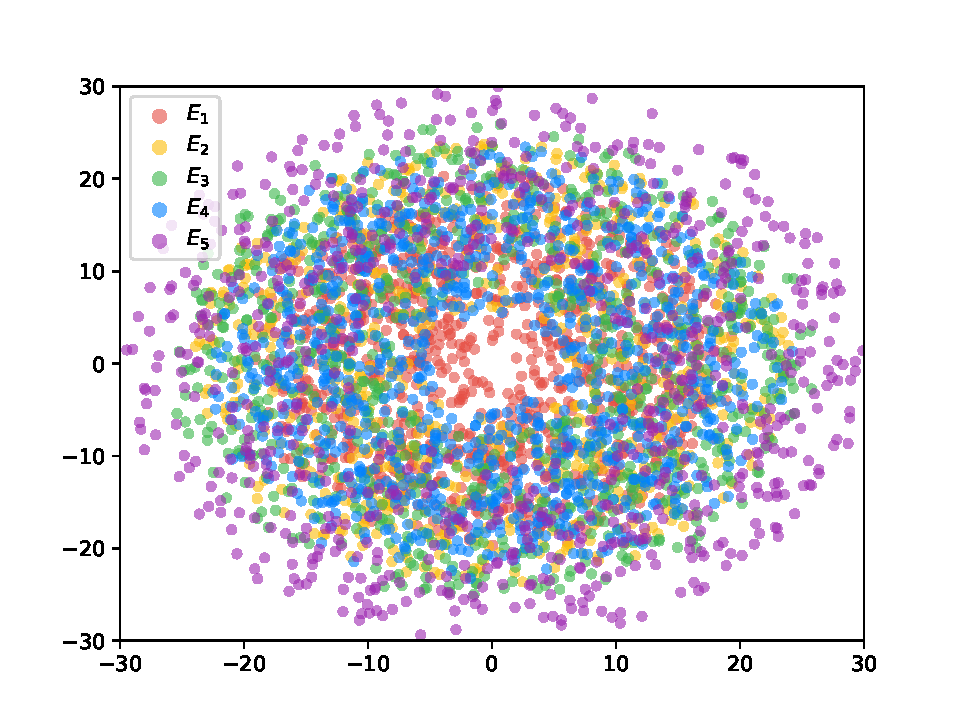
\includegraphics[width=0.4\textwidth]{2_RotatE_view.pdf}
    \label{Experiment1_figures_a}
  }
  \subfloat[NORMAN可视化结果]{
    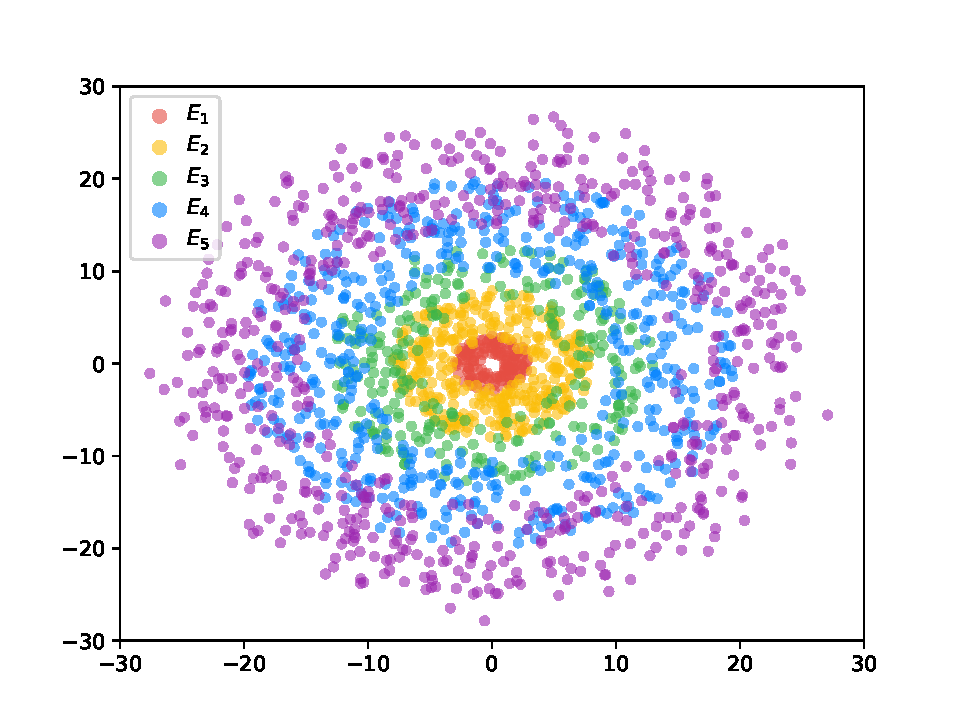
\includegraphics[width=0.4\textwidth]{2_NORMAN_view.pdf}
    \label{Experiment1_figures_b}
  }
  \caption{FB15K-237部分节点可视化结果}
  \label{Experiment1_figures}
\end{figure}
为了更直观地分析模型对知识图谱层次信息的表示效果,本文将RotatE模型和NORMAN模型对FB15K-237知识图谱的部分节点在欧氏空间中的表示向量进行了可视化展示,其中不同的节点采用不同颜色的点进行表示,得到的结果如图\ref{Experiment1_figures}所示。
可以发现,RotatE模型得到的知识图谱表示向量分布较为均匀,不能对不同层次的实体进行区分。
这种情况主要是因为RotatE模型采用的基于旋转的复数空间表示方法没有对知识图谱内的层次信息进行建模,因而不能够很好地体现知识图谱中的层次信息。
NORMAN模型得到的知识图谱表示向量则能够清晰地将不同层次的实体进行区分,可以看到图中不同的实体之间存在明显的层次划分,这主要是因为NORMAN模型采用的极坐标系编码器采用半径坐标对实体的层次级别进行表示,能够根据知识图谱中的层次信息为实体分配对应的半径坐标向量。
通过这种方法,NORMAN模型能够很好地捕获知识图谱中的层次信息,从而为知识推理等下游任务提供支持。


\section{本章小结}
本章主要介绍了基于因果推断的知识图谱表示学习模型,该模型能够将结构化三元组知识信息转换成向量表示。模型首先通过层次信息提取模块利用基于极坐标系的编码模型编码知识图谱,并通过聚类算法得到知识对应的层次信息。随后模型利用图神经网络模块,输入初始向量和知识层次信息,通过知识邻域信息传递进行数据更新,同时利用因果推断模块,根据层次差异得分、决策差异得分、预测置信度得分和推理距离得分等多种因素,评估各个图神经网络节点是否接收特定邻域的信息。
本章首先给出了知识图谱表示学习任务的定义,随后给出了方法概览并详细介绍了本文提出的基于因果推断的知识图谱表示学习模型与策略,最后在公开数据集上进行了实验,验证了模型的效果。


\chapter{基于双重智能体强化学习的知识推理模型}
本章提出一种基于双重智能体强化学习的知识推理模型LAURA,该模型使用实体和层次两种粒度的强化学习模块同时进行知识推理,并通过双重智能体强化学习交互模块实现信息交流和协作,共同实现高质量知识推理。
本章包含七个部分:知识推理任务定义(3.1节),模型方法概览(3.2节),实体级强化学习模块构建(3.3节),层次级强化学习模块构建(3.4节),双重智能体强化学习交互模块构建(3.5节),实验评估(3.6节),以及本章小结(3.7节)。

\section{知识推理任务定义}
知识推理任务的目标主要是基于现有知识,预测和推理新的知识的过程。根据知识推理步骤的长度,可以将知识推理方法分成两种,即单跳知识推理和多跳知识推理。
单跳知识推理的典型方法是直接通过知识图谱表示学习模型,采用知识图谱补全的方式实现知识推理,即给定查询三元组$\left(h, r, ?\right)$,$\left(h, ?, t\right)$或$\left(?, r, t\right)$,通过将知识图谱内所有关系或实体作为候选答案,输入到知识图谱表示学习模型中,从而将实体与关系映射到低维向量空间中,并通过得分函数进行打分,随后根据得分结果进行排序,选择得分最高的实体或关系作为答案,并完成知识推理。然而,上述单跳推理方法无法提供推理路径,这使得推理过程缺乏可解释性~\cite{wang2019deeppath}。
另一种推理方法,即多跳知识推理方法,能够利用知识图谱上的拓扑结构信息实现显式推理,并提供推理路径,因此具有更好的可解释性。多跳知识推理的典型方法是采用知识图谱表示学习和神经推理模型相结合的方式,首先获取知识图谱的初始表示,随后通过神经推理模型,从推理问题的初始实体开始,每次通过比较实体和邻域实体之间特定知识三元组的得分,获取得分最高的实体作为下一跳实体并进行后续推理,直到到达推理路径长度上限或到达目标实体为止。
在知识推理任务中,本章涉及到的符号及定义如表\ref{3_symbols}所示。
\begin{table}
  \centering
  \begin{tabular*}{0.4\textwidth}{@{\extracolsep{\fill}}clcl}
		\toprule[1pt]
    符号 & 描述\\ \hline
    $G$ & 知识图谱\\
    $F$ & 知识图谱事实集合\\
    $e$ & 实体变量\\
    $r$ & 关系变量\\
    $his$ & 历史信息变量\\
    $S$ & 状态信息\\
    $A$ & 动作空间\\
    $A^{add}$ & 额外动作空间\\
    $A^{co}$ & 协作动作空间\\
    $\pi_\theta$ & 策略网络\\
    $\pi_\theta^{co}$ & 协作策略网络\\
    $R$ & 奖励函数\\
    $\hat{R}$ & 轨迹相似度奖励\\
    $\operatorname{Similarity}(\cdot)$ & 相似度计算函数\\
		\bottomrule[1pt]
	\end{tabular*}
  \caption{本章符号定义}
  \label{3_symbols}
\end{table}

\section{基于双重智能体强化学习的知识推理模型框架概览}
本章提出的LAURA模型能够结合知识图谱表示学习模型,通过强化学习框架,实现多粒度和高质量的知识推理。图\ref{3_LAURA}展示了该模型,模型主要包含三个模块,分别是实体级强化学习模块、层次级强化学习模块和双重智能体强化学习交互模块。
对于实体级强化学习模块,该模块采用强化学习框架,在原始的实体级知识图谱上,由一个智能体(agent)根据策略网络(policy network)选取动作空间中的动作(action),改变自身状态(state),当到达结束条件时根据任务完成情况得到奖励(reward)。在此过程中,本文使用了第二章提出的知识图谱表示学习模型NORMAN,通过模型的知识图谱补全构建额外动作空间,从而降低知识图谱的稀疏情况对模型的影响。
% 本文还通过因果推断技术对动作空间进行了筛选,。
完成训练后,模块可以对查询的知识进行推理,返回知识的推理路径和对应的置信度。
对于层次级强化学习模块,该模块采用与实体级强化学习模块相同的强化学习框架,区别在于该模块使用的是层次知识图谱。首先利用知识图谱表示学习模型中的层次信息提取模块获取各个实体对应的层级,并将位于相同层级的全部实体作为层级节点,不同层级间则根据是否存在至少一条实体关联构建层级关联,从而完成层次知识图谱构建。随后可以在层次知识图谱上训练层次级强化学习模型。完成训练后,模块可以对给定知识进行推理,并返回层级级别的知识推理路径和对应置信度。
对于双重智能体强化学习交互模块,该模块为知识推理模型的核心模块,用于协调两个强化学习模块,实现模块间的信息交互。模块设计了协作动作空间、协作策略网络和轨迹相似度奖励两部分内容。协作动作空间是根据另一个模块的状态信息获取对应的动作内容以实现对动作空间的扩展,为两个模块能够具有相似的知识推理轨迹提供基础。协作策略网络是对模块策略网络的扩展,除了考虑自身模块当前状态、历史状态之外,还将另一个模块的历史状态纳入决策过程。轨迹相似度奖励是对模块奖励的扩展,除了考虑自身模块的奖励,还对两个模块的历史动作轨迹计算相似度得分,并与另一个模块的奖励一起作为补充奖励。完成训练后,模块可以在实体级和层次级两个级别进行知识推理,并将结果进行整合,返回置信度高于阈值的知识推理路径和对应的置信度信息。
需要注意的是,LAURA模型在开始知识推理前首先在实体级和层次级知识图谱的每个节点上添加了自环和反向边,从而使得智能体能够在知识图谱上进行双向推理,以及实现提前停止在某个节点上。
\begin{figure}
  \centering
  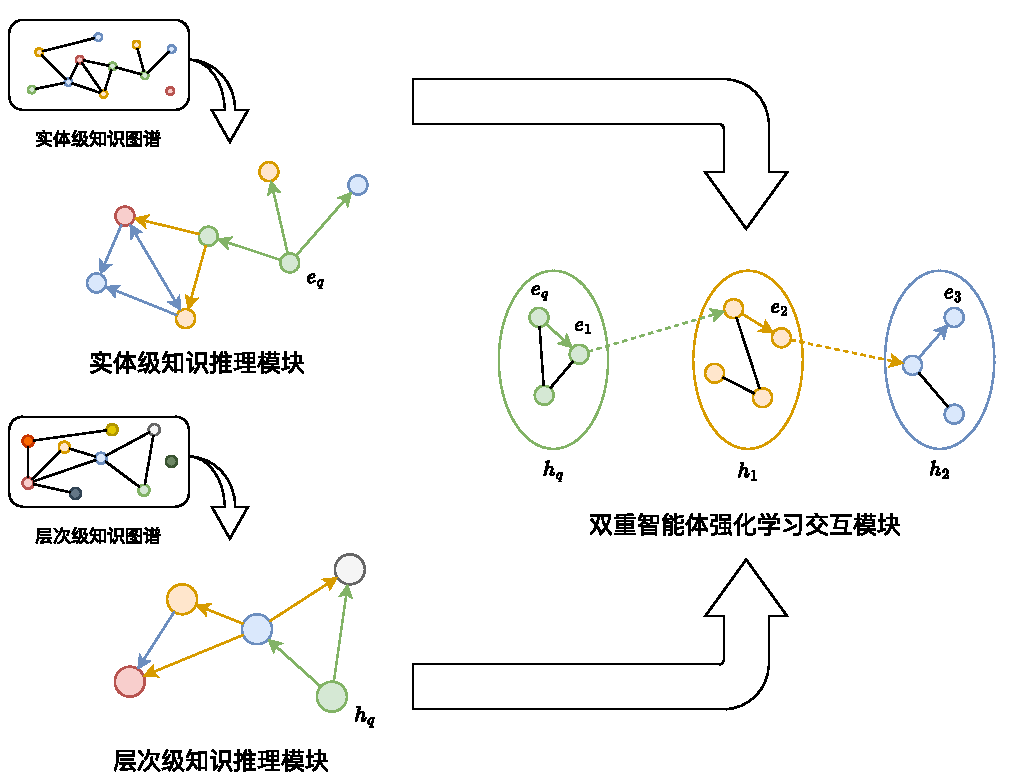
\includegraphics[width=0.7\textwidth]{3_LAURA}
  \caption{基于双重智能体强化学习的知识推理模型框架图}
  \label{3_LAURA}
\end{figure}

\section{实体级强化学习模块构建}
实体级强化学习模块用于在知识图谱上进行实体粒度的知识推理,模块采用强化学习框架,训练智能体在知识图谱上进行推理并最终得到目标实体,同时还可以通过智能体的移动轨迹获取相应的推理路径。此外,模块还采用第二章提出的知识图谱表示学习模型进行知识图谱补全,进而实现了动作空间的扩展。

本节在介绍实体级强化学习模块的过程中,首先进行模块概览的介绍,并针对知识推理过程的相关内容进行了分析。
随后介绍了模型的扩展动作空间,这部分使用了第二章提出的知识图谱表示学习模型,利用模型进行知识图谱补全,评估当前节点和其他节点之间存在链接的可能性,并选择高出阈值水平的作为新链接加入知识图谱中,从而实现动作空间的扩展。
% 随后介绍了模块采用的因果推断机制,该机制与第二章给出的因果推断模块类似,通过构建二元分类器评估能否选择相应的动作,完成动作空间的精简。
最后介绍实体级智能体学习过程,主要介绍了智能体的状态信息、动作空间、策略网络和奖励函数等内容。

\subsection{实体级强化学习模块概览}
实体级智能体的知识推理过程可以认为是一种马尔可夫决策过程(Markov Decision Process,MDP)~\cite{gronauer2022multi}。
可以将实体级智能体知识推理的过程表述为:给定知识图谱$G$的事实集合$F$和查询三元组$(h, r, ?)$(也可以是$(?, r, t)$和$(h, ? t)$的形式),其中已知的实体可以记作查询实体$e_q$或第0跳实体$e_0$,给定关系可以记作查询关系$r_q$。在强化学习框架中,智能体首先从查询实体$e_q$出发,不断选择知识图谱上的节点作为下一跳实体,直到到达跳数上限$L$为止,最终达到的实体即为答案实体,可以记作为答案实体$e_a$或第$L$跳实体$e_L$。
具体而言,在本节采用的实体级智能体知识推理的马尔可夫决策过程中,主要包含以下内容:
\begin{itemize}
  \item [1.] 状态信息$S$,主要用于表示智能体当前的状态情况。假设当前是智能体的推理过程的第$i$步,则智能体的状态信息可以表示为变量$\bm{s}_i = (\bm{e}_i, \bm{his}_i, \bm{e}_q, \bm{r}_q)$,其中$\bm{e}_i$表示第$i$步智能体所在实体的表示向量,$\bm{his}_i$表示智能体的历史轨迹信息表示向量,例如可以选择长短期记忆(Long Short-Term Memory,LSTM)模型编码智能体的历史轨迹并返回当前对应的表示向量$\bm{his}_i$,$\bm{e}_q$和$\bm{r}_q$则是查询实体和查询关系的表示向量,对单次查询而言是固定不变的信息。
  \item [2.] 动作空间$A$,是智能体当前所在实体节点$e_i$对应的知识图谱中全部出边构成的集合。当智能体处在实体节点$e_i$时,智能体的动作空间可以表示为变量$\bm{A}_i = \{(\hat{r}, \hat{e}) \mid (e_i, \hat{r}, \hat{e}) \in F\}$。
  \item [3.] 额外动作空间$A^{add}$,是本章提出的用于扩展常规动作空间的部分。考虑到部分知识图谱存在链接稀疏的情况,可能会造成模型无法进行有效推理,因此构建该部分内容。额外动作空间是采用历史路径和相同层次节点作为目标构建动作,并通过NORMAN模型的得分函数对动作进行筛选,最后完成额外动作空间的构建。构建的额外动作空间$\bm{A}_{i}^{add}$需要与动作空间$\bm{A}_i$合并,实现动作空间的更新,即$\bm{A}_i = \bm{A}_i + \bm{A}_{i}^{add} $。
  \item [4.] 策略网络$\pi_\theta$,用于建模智能体的动作选择策略。策略网络$\pi_\theta$可以根据智能体当前的状态信息$\bm{s}_i$和动作空间$\bm{A}_i$给出各个动作的概率分布$\pi_\theta(a \mid s_i, A_i), a \in A_i$,并通过随机采样的方式决定后续执行的动作。
  \item [5.] 状态转移过程,是智能体根据当前状态信息和动作空间,通过策略网络选择后续动作并更新状态信息的过程。当智能体根据策略网路选择了一个动作$a$后,有动作$a = (\hat{r}, \hat{e}), a \in A$以及实体$e_{i+1}=\hat{e}$,同时智能体会更新自身的状态信息$\bm{s}_{i+1} = (\bm{e}_{i+1}, \bm{his}_{i+1}, \bm{e}_q, \bm{r}_q)$。
  \item [6.] 奖励函数$R$,用于根据智能体最终是否到达正确答案而提供相应的奖励。通常情况下的奖励函数$R$是一个二值函数,如果智能体达到了正确答案则提供奖励为1,否则提供奖励为0。
\end{itemize}
由于策略网络$\pi_\theta$需要实体级和层次级强化学习模块共同构建,因此这部分内容将主要在后文的双重智能体强化学习交互模块进行介绍,其他部分则在本节进行介绍。构建的实体级强化学习模块如图\ref{3_EntityReinforcementLearning}所示。
\begin{figure}
  \centering
  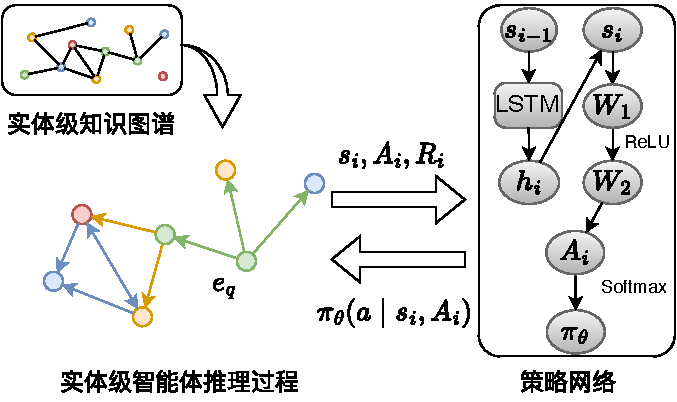
\includegraphics[width=0.6\textwidth]{3_EntityReinforcementLearning}
  \caption{实体级强化学习模块结构图}
  \label{3_EntityReinforcementLearning}
\end{figure}

\subsection{实体级智能体知识推理}
% \subsection{状态信息}
在构建实体级强化学习模块的状态信息$\bm{s}_i$时,考虑到模块的智能体需要能够获取三种信息,包括查询问题信息,当前节点信息和历史路径信息。其中,查询问题信息可以表示为查询三元组中的查询实体和查询关系对应的向量,即$\bm{e}_q$和$\bm{r}_q$。当前节点信息可以用当前实体对应的向量$\bm{e}_i$进行表示。对于历史路径信息,则考虑使用LSTM模型进行学习和表示,对应的向量获取过程为:
\begin{equation}
  \bm{his}_i=\operatorname{LSTM}\left(\bm{his}_{i - 1}, \bm{s}_{i - 1}\right), i \in [1, L_e], i \in \mathbb{Z}
  \label{equation_HistoryLSTM}
\end{equation}
根据上述计算过程,最终得到的状态信息可以表示为$\bm{s}_i = (\bm{e}_i, \bm{his}_i, \bm{e}_q, \bm{r}_q)$。

% \subsection{动作空间和额外动作空间}
动作空间的构造过程如前文所述,主要是根据智能体所处的节点位置$e_i$和知识图谱事实集合$F$的三元组信息实现构建,构建过程可以表示为:
\begin{equation}
  \bm{A}_i = \{(\hat{r}, \hat{e}) \mid (e_i, \hat{r}, \hat{e}) \in F\}
  \label{base_1}
\end{equation}
在进行动作空间构建时,考虑到知识图谱可能存在节点链接稀疏的情况,造成智能体无法沿着链接路径进行高质量知识推理。对此,本文考虑根据历史路径信息和层次信息对动作空间进行扩展,并通过知识图谱表示学习模型NORMAN评估候选实体是否可行,构造额外动作空间$\bm{A}_{i}^{add}$。具体方法是将历史路径节点和当前实体的相同层次节点构建节点集合$E_i$,同时根据关系集合$R$构造候选动作。得到的额外动作空间$\bm{A}_{i}^{add}$可以表示为:
\begin{equation}
  \bm{A}_{i}^{add} = \{(\hat{r}, \hat{e}) \mid (e_i, \hat{r}, \hat{e}) \notin G, \hat{r} \in R, \hat{e} \in E_i \}
  \label{extra_1}
\end{equation}
随后将$\bm{A}_{i}^{add}$的动作与$e_i$构造成三元组集合,选择NORMAN模型对三元组进行打分和筛选,仅保留得分最高的$T$个三元组对应的动作,从而完成额外动作空间的筛选。这里设置$\operatorname{Top@T}$为保留得分最高的$T$个三元组的函数,则筛选后的额外动作空间$\bm{A}_{i}^{add}$可以表示为:
\begin{equation}
  \bm{A}_i^{add} = \{(\hat{r}, \hat{e}) \mid \operatorname{Top@T}(f_{\hat{r}}(e_i, \hat{e})), (e_i, \hat{r}, \hat{e}) \notin G, \hat{r} \in R, \hat{e} \in E_i \}
\end{equation}
最后进行空间的融合$\bm{A}_i = \bm{A}_i \cup \bm{A}_{i}^{add} $,完成动作空间的扩展操作。

% \subsection{状态转移过程}
在完成上述状态信息$S$和动作空间$A$的构造后,在第$i+1$步推理过程时,智能体通过策略网络选择动作$a = (\hat{r}, \hat{e}), a \in A$,并从实体$e_i$移动到$e_{i+1} = \hat{e}$。随后,智能体会更新自身的状态信息$\bm{s}_{i+1} = (\bm{e}_{i+1}, \bm{his}_{i+1}, \bm{e}_q, \bm{r}_q)$,并进行下一步推理工作,直到达到最大步数$L_e$,即可得到答案实体$e_a$并完成知识推理过程。

% \subsection{奖励函数}
在构建奖励函数$R$的过程中,首先按照传统设置,当智能体达到正确答案时设置奖励为1,不能达到正确答案时设置奖励为0。考虑到智能体在大规模知识图谱进行长距离知识推理的过程中可能难以达到正确答案,从而造成奖励稀疏的问题,因此当智能体没有到达正确答案时,设置奖励函数$R$为第二章提出的知识图谱表示学习模型的得分函数,并将结果范围缩放到$[0, 1)$的范围。

% \subsection{因果推断过程}
% % 考虑到部分知识图谱的节点出度较多,使用基于强化学习框架的模型在进行知识推理时会遇到动作空间过大的情况,有必要进行动作空间的精简,筛除掉部分错误概率较大的动作。

\section{层次级强化学习模块构建}
\begin{figure}[t]
  \centering
  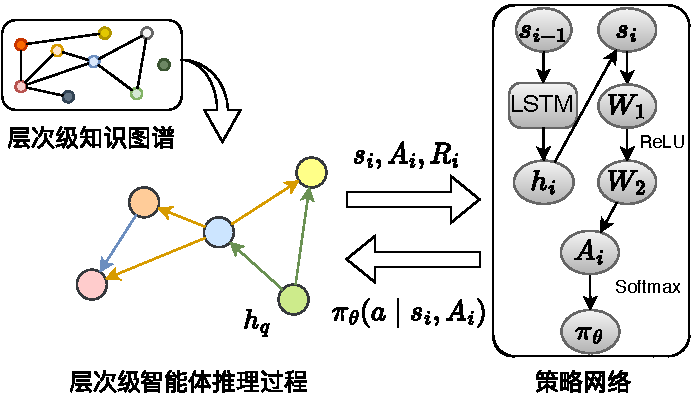
\includegraphics[width=0.6\textwidth]{3_LevelReinforcementLearning}
  \caption{层次级强化学习模块结构图}
  \label{3_LevelReinforcementLearning}
\end{figure}
本节提出的层次级强化学习模块,能够在层次级别上进行基于强化学习框架的路径推理,在推理过程中返回目标实体所在的层次级别,并提供相应的推理路径。在进行推理之前首先需要构建层次级知识图谱,随后采用强化学习框架进行模型训练,完成模块构建。

在介绍层次级强化学习模块的过程中,首先介绍了模块概览,给出了模块的结构图。随后介绍了层次级知识图谱的构建过程,通过采用第二章给出的层次信息提取模块可以获取知识图谱中实体的层次级别,从而实现层次级知识图谱的层次实体构建。同时可以根据初始知识图谱中实体间的关联信息构建层次级知识图谱实体间的边缘。最后介绍层次级智能体学习过程,在状态信息、动作空间、策略网络和奖励函数等多个内容角度上进行了介绍。


\subsection{层次级强化学习模块概览}
通常情况下的强化学习知识推理模型是通过知识图谱直接进行学习和推理的,因为知识图谱中的节点对应的是实体,因此这种推理也可以称作实体级的强化学习知识推理。
然而,实体级的强化学习推理通常缺乏宏观层面知识的引导,从而陷入局部循环或偏离目标实体。例如智能体所在的实体的邻域都是层次级别较低的实体,而目标实体的层次级别较高,则智能体可能会在低层次实体中陷入困境,无法达到目标实体。
为了给强化学习知识推理模型提供宏观层面的引导,有必要引入一种能够从全局的角度提供信息的模块,从而为实体级强化学习模型提供宏观信息并帮助智能体走出困境。

对此,本文提出了一种层次级强化学习模块。该模块的结构如图\ref{3_LevelReinforcementLearning}所示。
可以发现,模块的强化学习框架部分与实体级强化学习模块类似,与实体级强化学习模块不同的是层次级强化学习模块采用了层次知识图谱进行知识推理。
层次知识图谱主要是利用第二章提到的层次信息提取模块,通过获取知识图谱中各个实体的层次级别,并将层次级别相同的构建对应的层次级别节点,不同的层次级别节点之间如果存在实体关联,则构建对应的层次级别节点间关联。
通过上述步骤实现层次级知识图谱的构建,从而能够让层次级强化学习模块提供宏观知识引导,与实体级强化学习模块相辅相成。


\subsection{层次级知识图谱构建}
为了构建层次级的知识推理模型,首先需要根据知识图谱内实体的层次级别构建相应的层次级知识图谱。
本文选择继续使用第二章提到的层次信息提取模块,该模块采用基于极坐标系的知识图谱表示学习模型,能够将实体转换为极坐标系上的节点,并采用半径坐标向量表示实体的层次信息,角坐标向量区分同一层次的不同实体。
随后该模块能够通过K-Means聚类算法根据实体的半径坐标向量将实体划分为$K$个层次级别,其中$K$为超参数,可以根据知识图谱的可分层次情况进行调整。
根据该模块,可以将知识图谱内的实体划分为多个层次级别。将每个层次级别的全部实体视为单个层次级实体,即可得到层次级知识图谱的实体集合。
随后,如果两个层次内部至少有一个实体级关联存在,则连接对应的两个层次。通过上述方法可以完成层次级知识图谱的构建,构建过程如图\ref{3_LevelKG}所示。
基于该知识图谱即可进行层次级智能体的知识推理。
\begin{figure}
  \centering
  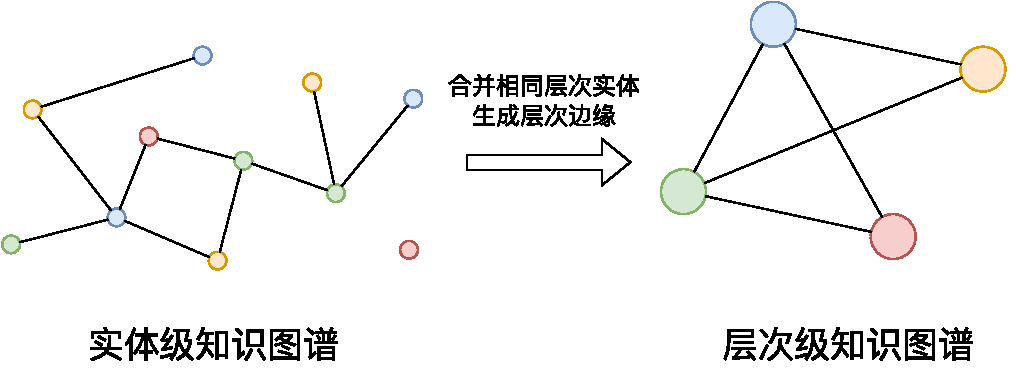
\includegraphics[width=0.6\textwidth]{3_LevelKG}
  \caption{层次级知识图谱构建过程}
  \label{3_LevelKG}
\end{figure}

\subsection{层次级智能体知识推理}
层次级和实体级的智能体知识推理过程基本一致,但是考虑到使用的是层次级知识图谱,因此在函数表示上略有差别。这里设层次级知识图谱内部的实体为$h$,即层次级别(hierarchical level)实体,其他表述与常规实体一致,如第$i$跳实体可以表示为$h_i$。
随后需要构造层次级智能体知识推理的状态信息、动作空间和状态转移过程。

% \subsection{状态信息}
构建层次级强化学习模块的状态信息$\bm{s}_i$时依然采用三种信息进行表示,分别是查询问题信息、当前节点信息和历史路径信息。由于层次级知识图谱中的关系主要是描述不同层次集合之间是否有内部联系,难以直接对查询三元组的查询关系$r_q$进行直接表示,因此在查询问题信息部分不加入查询关系信息,仅包含查询实体信息。同时,查询实体信息需要调整为层次知识图谱的查询层次实体信息对应的向量,表示为$\bm{h}_q$。当前节点信息用当前层次实体对应的向量$\bm{h_i}$表示。历史路径信息同样适用LSTM模型进行学习和表示,构造过程如公式\ref{equation_HistoryLSTM}所示。最终构造的状态信息可以表示为$\bm{s}_i = (\bm{h_i}, \bm{his}_i, \bm{h}_q)$。

% \subsection{动作空间和额外动作空间}
在进行动作空间的构造时,动作空间主要是根据智能体所处位置$h_i$和层次知识图谱$G_h$的事实信息集合$F_h$进行构造,构造过程可以表示为:
\begin{equation}
  \bm{A}_i = \{(\hat{r}, \hat{h}) \mid (h_i, \hat{r}, \hat{h}) \in F_h\}
  \label{base_2}
\end{equation}
由于层次知识图谱的节点较少,同时节点间的关系是根据节点内部实体是否存在关联而构建的,因此节点间的链接较多,智能体能够在稠密的知识图谱上进行遍历。因此在构造层次级知识图谱模块的动作空间时不对动作空间进行额外的扩充。

% \subsection{状态转移过程}
在完成上述状态信息$S$和动作空间$A$的构造后,层次级智能体即可在知识推理的过程中进行状态转移。在第$i+1$步推理的过程中,层次级智能体通过策略网络选择动作$a = (\hat{r}, \hat{h}), a \in A$,并从层级实体$h_i$转移到$h_{i+1}$。随后,更新层次级智能体对应的状态信息$\bm{s}_{i+1} = (\bm{h_{i+1}}, \bm{his}_{i+1}, \bm{h}_q)$,并在随后进行后续推理过程,直到达到最大推理步数$L_h$,即可得到答案层次实体$h_a$,完成推理过程。

% \subsection{奖励函数}
最后进行奖励函数$R$的构造。由于层次知识图谱的节点数量较少,智能体通过知识推理达到正确的层次节点的概率相对于实体级知识推理任务更高,因此层次级知识推理模块的奖励函数采用传统设计,即智能体最终到达正确实体所在的层次节点则奖励为1,没有到达正确实体所在层次节点则奖励为0。

\section{双重智能体强化学习交互模块构建}
在此前的基于强化学习的知识推理方法中,模型通常可以有效地在知识图谱上进行短距离推理,但在进行长距离推理时,智能体往往因为缺少引导信息而偏离目标实体,导致无法获得正确的推理目标。
为了解决这一问题,本文提出的基于双重智能体强化学习的知识推理模型分别训练实体级和层次级的强化学习模块,并通过双重智能体强化学习交互模块实现两个模块的交互,由层次级强化学习模块捕获全局性的和层次级别的知识,实体级强化学习模块捕获局部性的和实体级别的知识,两者通过协作动作空间、协作策略网络和轨迹相似度奖励机制,相互促进和引导,共同实现知识推理过程,从而在进行长距离推理时能够有效地确定目标实体,提高知识推理准确率。

本节在介绍双重智能体强化学习交互模块的过程中,首先给出了模块概览并提供了模块结构图。
随后介绍并分析了模块如何通过协作动作空间、协作策略网络和轨迹相似度奖励实现了实体级和层次级强化学习模块的信息交互。
最后介绍了双重智能体智能体的学习过程,给出了模块的知识推理算法。

\subsection{双重智能体强化学习交互模块概览}
前面介绍的两种粒度的强化学习模块均能够独立进行学习和训练,然而在知识推理效果上来看,实体级强化学习模块属于传统的强化学习知识推理方法,同时层次级强化学习模块只能进行层次级别的知识推理并最终确定答案实体所在的层次级别,而不能确定真正的答案实体是哪一个。
因此,为了提高知识推理的效果,有必要将上述两种知识推理模型融合起来,实现一种基于双重智能体强化学习的知识推理模型。

为了实现上述目标,本文设计了双重智能体强化学习交互模块。模块的结构如图\ref{3_DualReinforcementLearning}所示。
可以发现,模块的输入是实体级和层次级强化学习模块部分获取的状态信息和动作空间,首先通过构建协作动作空间扩展两种智能体的动作空间,使得智能体有能力获取相似的推理轨迹。
随后在双重智能体强化学习交互模块中通过协作策略网络综合两个模块的信息选择后续动作并进行状态转移。
当推理达到最大跳数并获得最终的答案实体后,通过双重智能体强化学习交互模块的轨迹相似度奖励评估两个模块智能体是否能够按照相似的轨迹进行推理,并与两个模块自身的奖励函数相结合,为智能体提供奖励。
通过本节提出的双重智能体强化学习交互模块,能够实现两种粒度的知识推理模块间的交互,进而增强知识推理效果。
\begin{figure}
  \centering
  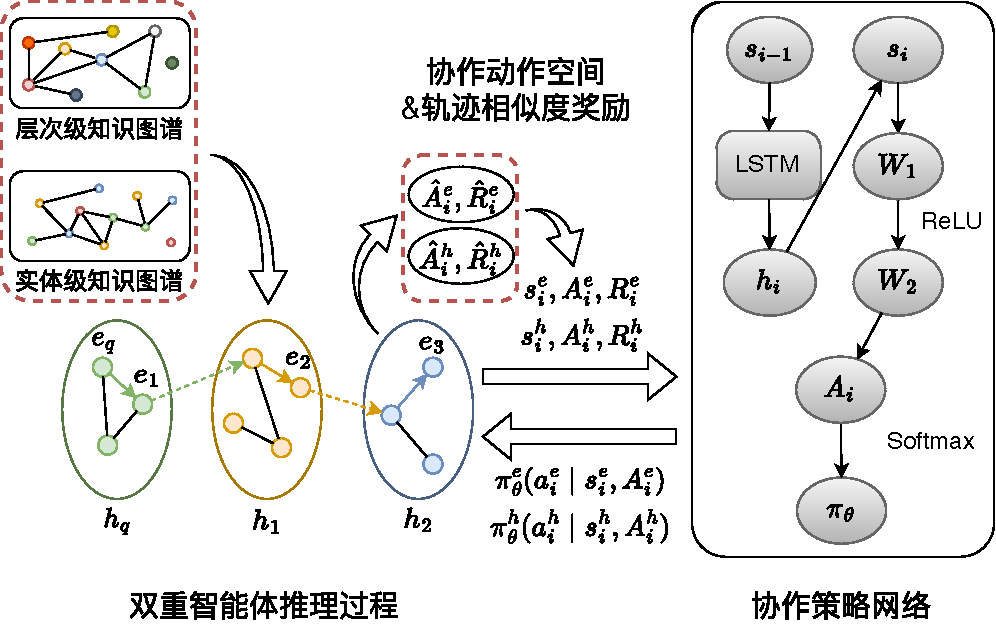
\includegraphics[width=0.7\textwidth]{3_DualReinforcementLearning}
  \caption{双重智能体强化学习交互模块结构图}
  \label{3_DualReinforcementLearning}
\end{figure}

\subsection{协作动作空间}
本章在实体级和层次级强化学习模块曾介绍过智能体的动作空间$A$是根据知识图谱提供的知识信息构造的动作集合,可以表示为变量$\bm{A}_i = \{(\hat{r}, \hat{e}) \mid (e_i, \hat{r}, \hat{e}) \in F\}$,同时可以考虑构造额外动作空间$A^{add}$实现对动作空间$A$的扩展。
为了增强两种模型的交互性,让两种模型的推理轨迹等信息能够相互交互,本节提出了协作动作空间的方法,这种方法为每种智能体分别构造额外动作空间,用于覆盖另一种智能体所在的节点对应的内容。通过这种方法能够让两种智能体的动作空间相互交融,为两种智能体沿着相似的道路进行推理提供必要条件。
这里采用上角标$e$和$l$分别表示实体级和层次级智能体对应的内容,$\bm{\hat{A}}_i$表示第$i$步的协作动作空间,则实体级智能体在第$i$步的协作动作空间可以表示为:
\begin{equation}
  \bm{\hat{A}}_i^{e} = \{(\hat{r}, \hat{e}) \mid \hat{r} \in R, \hat{e} \in \operatorname{Entity}(h_i)\}
  \label{coo_1}
\end{equation}
其中,$\operatorname{Entity}(\cdot)$函数表示获取层次节点对应的实体内容。通过上述函数,实体级智能体的协作动作空间$\bm{\hat{A}}_i^{e}$可以覆盖层次级智能体所在的层次节点对应的所有实体节点,从而让实体级智能体具有沿着层次级智能体的路径继续前进的能力。
类似的,可以构造层次级智能体在第$i$步的协作动作空间为:
\begin{equation}
  \bm{\hat{A}}_i^{h} = \{(\hat{r}, \hat{h}) \mid \hat{r} \in R_h, \hat{h} \in \operatorname{Hierarchy}(e_i)\}
  \label{coo_2}
\end{equation}
其中,$\operatorname{Hierarchy}(\cdot)$函数表示获取实体节点对应的层次级别。通过上述函数,层次级智能体的协作函数$\bm{\hat{A}}_i^{h}$也可以覆盖实体级智能体所在的实体节点对应的层次节点,从而为层次级智能体能够根据实体级智能体提供的微观信息沿着相似的道路前进提供了支持。
最后,将协作动作空间合并到动作空间,可以表示为:
\begin{equation}
  \begin{aligned}
    \bm{A}_i^{e} &= \bm{A}_i^{e} \cup \bm{\hat{A}}_i^{e} \\
    \bm{A}_i^{h} &= \bm{A}_i^{h} \cup \bm{\hat{A}}_i^{h}
  \end{aligned}
\end{equation}

\subsection{协作策略网络}
在协作策略网络中,我们的主要目标是根据实体级和层次级知识推理模块的智能体状态信息和动作空间,形成一种协作策略函数,能够为实体级和层次级智能体提供相应的动作概率,并通过采样选择后续的动作。
在具体的实践过程中,考虑到前文介绍到智能体的状态信息可以表示为$\bm{s}_i = (\bm{e}_i, \bm{his}_i, \bm{e}_q, \bm{r}_q)$,其中$\bm{e}_i, \bm{e}_q, \bm{r}_q$分别是第$i$步智能体所在实体信息和查询实体及关系信息,这些信息基本只与智能体自身有关,难以与另一个智能体进行信息交互。而历史信息$\bm{his}_i$可以通过调整,与另一个智能体产生关联,从而进行信息交互。
因此,本文设计的协作策略网络主要是调整实体级和层次级智能体对应的历史信息,使得每种智能体的历史信息都包含了另一个智能体的历史信息,构造协作历史信息$\bm{his}^{co}$并由两种智能体所共享。这里设最大跳数为$L$,同时采用上角标$e$和$l$分别表示实体级和层次级智能体对应的内容,则智能体第$i$步的协作历史信息$\bm{his}_i^{co}$可以表示为:
\begin{equation}
  \bm{his}_{i}^{co} = \left[\bm{his}_{i-1}^e, \bm{his}_{i-1}^l\right], \quad i \in [1, L] \  \And \  i \in \mathbb{Z}
  \label{his_1}
\end{equation}
随后,采用LSTM模型对节点的之前状态和协作历史信息一起进行编码,即可获得智能体的历史信息。
实体级智能体的历史信息向量的计算过程可以表示为:
\begin{equation}
  \begin{aligned}
    \bm{his}_0^e &= \operatorname{LSTM}^e\left(\bm{0}, \bm{0}\right) \\
    \bm{his}_i^e &= \operatorname{LSTM}^e\left(\mathbf{W}^e \cdot \bm{his}_i^{co}, \bm{s}_{i-1}^e\right),\quad i \in [1, L_e] \  \And \  i \in \mathbb{Z}
  \end{aligned}
  \label{his_2}
\end{equation}
可以采用相似的方法求得层次级智能体的历史信息向量为:
\begin{equation}
  \begin{aligned}
    \bm{his}_0^l &=\operatorname{LSTM}^l\left(\bm{0}, \bm{0}\right) \\
    \bm{his}_i^l &= \operatorname{LSTM}^l\left(\mathbf{W}^l \cdot \bm{his}_i^{co}, \bm{s}_{i-1}^l\right),\quad i \in [1, L_h] \  \And \  i \in \mathbb{Z}
  \end{aligned}
  \label{his_3}
\end{equation}
完成构建协作历史信息后,即可进一步构建协作策略网络。这里设置实体级智能体的状态信息向量为$\bm{s}_i^{e} = \left[\bm{e}_q, \bm{r}_q, \bm{e}_i, \bm{his}_i^e\right]$,则构建的实体级智能体的协作策略网络可以表示为:
\begin{equation}
  \pi_\theta^e\left(\bm{a}_i^e \mid \bm{s}_i^e, \bm{A}_i^e\right) =\operatorname{Softmax}\left(\bm{A}_i^e \times \mathbf{W}_1^e \operatorname{ReLU}\left(\mathbf{W}_2^e \cdot \bm{s}_i^{e}\right)\right)
  \label{pi_1}
\end{equation}
类似的,设置层次级智能体状态信息向量为$\bm{s}_i^{h} = \left[\bm{h}_q, \bm{h}_i, \bm{his}_i^l\right]$,可以构建层次级智能体的协作策略网络。
\begin{equation}
  \pi_\theta^l\left(\bm{a}_i^l \mid \bm{s}_i^l, \bm{A}_i^l\right) =\operatorname{Softmax}\left(\bm{A}_i^l \times \mathbf{W}_1^l \operatorname{ReLU}\left(\mathbf{W}_2^l \cdot \bm{s}_i^{h}\right)\right)
  \label{pi_2}
\end{equation}
通过上述协作策略网络,可以为智能体提供动作空间内各项动作的概率,并通过采样的方式,获取后续动作,实现知识推理。在这些步骤中,通过构建协作历史信息$\bm{his}^{co}$,可以让两个知识推理模块共享历史路径信息,从而有助于帮助它们协作推理,共同解决问题。具体而言,层次级智能体会提供给实体级智能体层次层面的信息,帮助实体级智能体确定接下来的动作应该朝着哪个层级的目标进步。另一方面,实体级智能体会为层次级智能体分享自己的动作轨迹,帮助层次级智能体了解后续动作应该朝带有何种实体特征的层级节点前进,从而实现相互帮助。

\subsection{轨迹相似度奖励}
为了实现实体级和层次级知识推理模块的信息交互,本节还针对奖励函数做了新的设计,即轨迹相似度奖励。
通过协作动作空间,为两种智能体沿着相似的轨迹行进提供了基础保障条件。随后构建的协作策略网络,有助于两种智能体交换信息。
但是上述方法不能明确地指导两种智能体需要沿着相似的路径进行推理,两种智能体依然是只考虑自身能否到达目标节点,而没有考虑帮助另一个智能体达到正确的节点。
为了进一步增强两种智能体的协作,本节设计的轨迹相似度奖励能够作为一种补充奖励,鼓励两种智能体沿着相似的路径推理。
轨迹相似度奖励的思路主要是:对两种智能体推理的路线进行相似度计算,并获取相似度得分。
此外,还需要加上另一种智能体的原始得分,以评估是否引导信息能够帮助另一个智能体得到正确的答案。
在计算的过程中,采用$\hat{R}_i$表示第$i$步的轨迹相似度奖励得分,则实体级智能体的轨迹相似度奖励可以表示为:
\begin{equation}
  \hat{R}^e = \sum_{i=1}^{L} \operatorname{Similarity}(\bm{e}_i, \bm{h}_i) + R^h
  \label{similar_1}
\end{equation}
其中$\operatorname{Similarity}(\cdot)$是相似度评估函数,主要计算方法是对输入的两个向量的余弦相似度进行计算。
类似的,可以构建层次级智能体的轨迹相似度奖励:
\begin{equation}
  \hat{R}^h = \sum_{i=1}^{L} \operatorname{Similarity}(\bm{e}_i, \bm{h}_i) + R^e
  \label{similar_2}
\end{equation}
最后,对两种智能体的奖励函数进行更新,即可完成奖励函数的补充:
\begin{equation}
  \begin{aligned}
    R^e &= R^e + \hat{R}^e \\
    R^h &= R^h + \hat{R}^h
  \end{aligned}
  \label{similar_reward}
\end{equation}
% 其中,$\beta_1$和$\beta_2$用于调整轨迹相似度奖励的权重。

轨迹相似度奖励能够通过计算轨迹的余弦相似度,评估两种智能体是否沿着近似的道路进行推理。同时,考虑了另一种智能体最终的得分,保证了轨迹相似度奖励能够在保证推理路径相同的情况下兼顾对另一个智能体正确性的观察。
通过引入轨迹相似度奖励,能够让两种智能体能够学习通过相互沟通信息,并共同沿着相似的路径进行推理,提高了推理的一致性。另一方面,轨迹相似度奖励还有助于缓解大规模知识图谱中应用强化学习框架的奖励稀疏问题,提高模型的学习速度。

\subsection{双重智能体知识推理}
本节提出的双重智能体强化学习交互模块是知识推理模型LAURA的核心模块,通过协作动作空间、协作策略网络和轨迹相似度奖励,将实体级和层次级知识推理模块结合了起来,确保两种模块能够接受对方信息并沿着对方相似的推理路径进行知识推理,实现了宏观和微观信息的紧密交流和结合,从而能够进行双重智能体知识推理。
基于双重智能体强化学习的知识推理模型LAURA的训练过程如算法\ref{algorithm_dualagent}所示。
\begin{algorithm}[H]
	\caption{LAURA模型训练算法}  
	\label{algorithm_dualagent}
	\begin{algorithmic}[1]
  \Require 知识图谱事实集合$F$, 数据集$D$, 模型$NORMAN$, 最大范围$L$, 学习率$\alpha$
  \Ensure 实体级智能体策略网络$\pi_\theta^e$, 层次级智能体策略网络$\pi_\theta^l$
  \For{$(e_q, r_q, e_a) \in D$}
  \State $(h_q, h_a) \leftarrow \operatorname{GetHierarchy}(e_q, e_a)$ // 通过层次信息提取模块获取层次信息
  \State $\bm{s}_{0}^{e} \leftarrow (\bm{e}_q, \bm{0}, \bm{e}_q, \bm{r}_q), \bm{s}_{0}^{l} \leftarrow (\bm{h}_q, \bm{0}, \bm{h}_q)$ // 初始化实体级和层次级状态信息
  \State $\bm{A}_{0}^{e} \leftarrow \operatorname{GetActionSpace}(e_0, F) \cup \operatorname{GetExtraSpace}(e_0, NORMAN) \cup \operatorname{GetCooperationSpace}(e_0, h_0)$ // 根据公式\ref{base_1}, \ref{extra_1}和\ref{coo_1}获取实体级动作空间
  \State $\bm{A}_{0}^{l} \leftarrow \operatorname{GetActionSpace}(h_0, F) \cup \operatorname{GetCooperationSpace}(h_0, e_0)$ // 根据公式\ref{base_2}和\ref{coo_2}获取层次级动作空间
  \For{$i \leftarrow 1$ to $L$}
  \State $\bm{e}_i \leftarrow \operatorname{Sample}(\pi_\theta^e(\bm{s}_{i-1}^{e}, \bm{A}_{i-1}^{e}))$
  \State $\bm{h}_i \leftarrow \operatorname{Sample}(\pi_\theta^l(\bm{s}_{i-1}^{l}, \bm{A}_{i-1}^{l}))$
  \State $\bm{his}_{i}^{coo} \leftarrow \operatorname{GetHistory}(\bm{his}_{i-1}^{e}, \bm{his}_{i-1}^{l})$ // 根据公式\ref{his_1}获取协作历史信息
  \State $\bm{his}_{i}^{e} \leftarrow \operatorname{GetEntityHistory}(\bm{his}_{i}^{coo}, \bm{e}_{i-1})$ // 根据公式\ref{his_2}获取实体级历史信息
  \State $\bm{his}_{i}^{l} \leftarrow \operatorname{GetLayerHistory}(\bm{his}_{i}^{coo}, \bm{h}_{i-1})$ // 根据公式\ref{his_3}获取层次级历史信息
  \State $\bm{s}_{i}^{e} \leftarrow (\bm{e}_{i}, \bm{his}_{i}^{e}, \bm{e}_q, \bm{r}_q)$ // 更新实体级状态信息
  \State $\bm{s}_{i}^{l} \leftarrow (\bm{h}_{i}, \bm{his}_{i}^{l}, \bm{h}_q)$ // 更新层次级状态信息
  \State $\bm{A}_{i}^{e} \leftarrow \operatorname{GetActionSpace}(\bm{e}_i, F) \cup \operatorname{GetExtraSpace}(\bm{e}_i, NORMAN) \cup \operatorname{GetCooperationSpace}(\bm{e}_i, \bm{h}_i)$ // 更新实体级动作空间
  \State $\bm{A}_{i}^{l} \leftarrow \operatorname{GetActionSpace}(\bm{h}_i, F) \cup \operatorname{GetCooperationSpace}(\bm{h}_i, \bm{e}_i)$ // 更新层次级动作空间
  \EndFor
  \State $R^{e} \leftarrow \operatorname{GetEntityReward}(\bm{e}_L, \bm{e}_a, NORMAN) + \operatorname{GetSimilarReward}_{i=1,\cdots,L}(\bm{e}_i, \bm{h}_i, R^{l})$// 根据公式\ref{similar_1}和\ref{similar_reward}计算实体级奖励
  \State $R^{l} \leftarrow \operatorname{GetLayerReward}(\bm{h}_L, \bm{h}_a) + \operatorname{GetSimilarReward}_{i=1,\cdots,L}(\bm{e}_i, \bm{h}_i, R^{e})$// 根据公式\ref{similar_2}和\ref{similar_reward}计算层次级奖励
  \State $\pi_\theta^e \leftarrow \operatorname{UpdateEntity}(\pi_\theta^e, R^{e}, \alpha)$// 更新实体级策略网络
  \State $\pi_\theta^l \leftarrow \operatorname{UpdateEntity}(\pi_\theta^l, R^{l}, \alpha)$// 更新层次级策略网络
  \EndFor
  \State \Return $\pi_\theta^e, \pi_\theta^l$
	\end{algorithmic}
\end{algorithm} 

\section{实验评估}
本节在多个开源数据集上开展实验,综合评估LAURA模型的性能。
LAURA模型使用Python语言编写,Python版本为3.10.1,使用的深度学习框架为PyTorch,版本为1.13.1。
同时,本节所有实验都是在型号为AMAX G448-X3的服务器上完成的,服务器的具体参数包括:CPU型号为Xeon Sliver 4314,GPU型号为GeForce RTX 3090,系统内存为64G,系统硬盘为500G,操作系统版本为Ubuntu 22.04.1 LTS。

\subsection{实验概览}
知识推理模型的目标是基于知识图谱中的已有知识预测和推理新的知识。为了评估知识推理模型的效果,我们选择了单跳知识图谱问答和多跳知识图谱问答两种实验来进行模型评估。
在单跳知识图谱问答任务中,知识推理模型可以直接采用查询语句进行单跳知识推理,对于不能直接知识推理的模型则首先需要通过知识抽取将查询语句转换成查询三元组$(h, r, ?)$,$(?, r, t)$或$(h, ?, t)$,随后的知识推理过程和知识图谱补全的过程较为相似,通过知识推理模型对所有候选答案进行评分,这里的获取得分有多种方法,可以是知识图谱表示学习模型的得分函数,也可以是强化学习等推理模型通过计算得到的置信度得分。最后按照得分的降序顺序对候选三元组进行排序,并根据结果三元组序列评估模型效果。
多跳知识图谱问答则相对更加复杂一些。知识推理模型可以直接采用查询语句进行多跳知识推理,对于不能直接知识推理的模型也是需要将查询语句转换成查询三元组$(h, r, ?)$,$(?, r, t)$或$(h, ?, t)$,随后要求模型根据已有的知识图谱进行查询,在指定跳数$T$的范围内进行多跳推理,最后对所有候选答案进行得分计算,同样是对得分进行降序排序,并根据最终排序结果评估模型效果。

在构造查询语句时,本文首先采用了与知识图谱补全任务相似的方式,通过随机移除知识图谱事实三元组$(h, r, t)$中的任意一项构造查询三元组。
随后需要利用查询三元组构造对应的查询语句,考虑到实验的主要目的是考察模型的知识推理效果而不是知识抽取效果,因此本文采用固定的模板构造统一格式的查询语句。对于$(h, r, ?)$格式的查询三元组,构造的查询语句为“\textit{$h$的$r$是什么?}”。对于$(?, r, t)$格式的查询三元组,构造的查询语句为“\textit{$t$的$r^{-1}$是什么?}”,其中$r^{-1}$表示关系$r$的逆关系。对于$(h, ?, t)$格式的查询三元组,构造的查询语句为“\textit{$h$和$t$的关系是什么?}”。通过上述模板,可以将查询三元组转换为查询语句。同时,模型采用的知识抽取过程也是采用模板匹配的方法,通过对上述查询语句应用模板进行匹配获取对应的查询三元组,并完成后续的知识推理工作。
本文选择的知识图谱问答的评价指标同样为平均排序MR、平均倒数排序MRR和Hits@K等,根据知识图谱补全实验的分析,一般认为平均倒数排序MRR的表示能力优于平均排序MR,因此本文选择平均倒数排序MRR和Hits@K作为评估指标。

本节首先介绍了知识推理模型的评估实验内容,即通过单跳知识图谱问答和多跳知识图谱问答,评估模型的效果。随后介绍了任务的评价指标、数据集和具体的实验设置,并在最后比较本文提出的LAURA模型和其他基线知识推理模型在知识图谱问答上的效果,进而对LAURA模型的优势和劣势进行客观评估。

\subsection{数据集}
本文在单跳知识图谱问答和多跳知识图谱问答两种任务上进行模型评估。
针对单跳知识图谱问答,本文采用的数据集包括:FB15K-237、WN18RR和NELL-995。
另一方面,对于多跳知识图谱问答,本文采用的数据集包括:FB15K-237-10\%、FB15K-237-20\%和FB15K-237-50\%~\cite{lv2020dynamic}。%NELL23K和WD-singer~\cite{lv2020dynamic}。
在单跳知识图谱问答中,由于单跳知识图谱问答与知识图谱补全任务对数据集的要求是相同的,因此本文选择与知识图谱表示学习模型实验部分相同的数据集,即FB15K-237、WN18RR和NELL-995,从而能够更好的对本文提出的两种模型进行对比。
在多跳知识图谱问答任务中,考虑到多条推理过程需要综合一定范围内的知识进行综合评估,为了测试本文提出的模型在不同稀疏程度的知识图谱上的性能,本文选择了多个基于FB15K-237数据集进行随机采样得到的数据集,即FB15K-237-10\%、FB15K-237-20\%和FB15K-237-50\%。由名字可以看出,这三个数据集分别随机保留了FB15K-237数据集的10\%、20\%和50\%的三元组数据,从而能够评估模型利用不同稀疏程度的知识图谱进行知识推理的能力。
% 此外,对于多跳推理任务,本文还选择了NELL23K和WD-singer这两个数据集。
% NELL23K数据集是根据大规模知识图谱NELL中进行采样得到的数据集。具体而言,NELL23K提供了22925种实体和200种关系,同时提供了35358条三元组数据。可以看到,NELL23K的实体数据种类较多,同时三元组数量较少,这增加了训练模型的难度,需要模型根据实体种类以外的其他信息进行知识图谱问答。
% WD-singer数据集是从维基百科知识图谱Wikidata中采样的数据集,与上述其他数据集不同,WD-singer仅包含Wikidata中与歌手相关的内容,首先获取歌手相关的概念,随后通过这些概念获取对应的实体,构建实体列表。最后搜索包含实体列表中实体的三元组,形成最终数据集。WD-singer提供了10282种实体和135种关系,并提供了20508条三元组。可以发现WD-singer同样较为稀疏,可以考察模型对稀疏知识图谱的推理能力。
具体统计数量上,本部分采用的单跳推理测试数据集的统计数据见表\ref{Datasets1},多跳推理测试数据集如表\ref{Datasets2}所示。根据上文分析可知,本文选择的单跳和多跳知识图谱问答数据集能够较好的评估模型的知识推理能力,同时能够评估模型在不同稀疏程度的知识图谱上的效果。

\begin{table}
  \centering
  \begin{tabular*}{0.95\textwidth}{@{\extracolsep{\fill}}lccccc}
		\toprule[1pt]
    数据集 & 实体数量 & 关系数量 & 训练集数量 & 验证集数量 & 测试集数量 \\ \hline
    FB15K-237-10\% & 11512 & 237 & 27211 & 15624 & 18150\\
    FB15K-237-20\% & 13166 & 237 & 54423 & 16963 & 19776\\
    FB15K-237-50\% & 14149 & 237 & 136057 & 17449 & 20324\\
    % NELL23K & 22925 & 200 & 31822 & 1768 & 1768\\
    % WD-singer & 10282 & 135 & 18458 & 1025 & 1025\\
		\bottomrule[1pt]
	\end{tabular*}
  \caption{多跳知识图谱问答数据集统计信息}
  \label{Datasets2}
\end{table}

\subsection{实验设置}
在使用LAURA模型进行单跳和多跳知识图谱问答实验前,首先需要对模型的超参数进行设置。本文对LAURA模型的超参数进行了调整,并最终形成了一系列最优超参数。
首先,需要针对强化学习框架设置各个模块通用的超参数。这里设置最大出边度数为200,最大动作空间为256,实体对最大边数为10,实体嵌入维度为512,嵌入丢弃率为0.3,前馈层丢弃率为0.1,历史网络层数为3,历史嵌入维度为128,衰减率为0.05,延迟复制步数为5,采样部署频率为3,训练批次大小为128。
考虑到各个数据集的数据量大小和结构差异,针对不同的数据集还需要设置对应的动作丢弃率、集束搜索(beam search)大小和学习率$\alpha$。
在实体级强化学习模块需要设置的超参数主要是最大跳数$L_e$和补充动作空间大小$T$。这里我们统一设置$L_e = 3$。
类似的,在层次级强化学习模块需要对层次级智能体知识图谱问答的最大跳数$L_h$进行设置。同样也是设置为$L_h = 3$。
% 在双重智能体强化学习交互模块,主要需要设置实体级和层次级智能体轨迹相似度奖励权重,分别为$\beta_1$和$\beta_2$。
由于LAURA需要使用NORMAN模型提供知识图谱层次信息,以及使用NORMAN模型的得分函数作为补充奖励,因此还需要对NORMAN模型的超参数进行设置。考虑到单跳知识图谱问答同样使用了FB15K-237、WN18RR和NELL-995数据集,因此采用的超参数设置情况与表\ref{Hyperparameters1}相同。多跳知识图谱问答部分则需要重新设置对应的NORMAN模型超参数。在对FB15K-237-10、FB15K-237-20和FB15K-237-50进行超参数调整和实验评估后,最后的超参数仍然与FB15K-237一致,这说明上述三种FB15K-237的子数据集在构建的时候符合均匀采样的原则,使得构建出的子数据集仍然可以采用同样的超参数取得最好的效果。
实验针对单跳知识图谱问答和多跳知识图谱问答分别调整对应超参数,得到的超参数设置情况分别如表\ref{Hyperparameters2_Singlehop}和表\ref{Hyperparameters2_Multihop}所示。

\begin{table}[]
  \centering
  \begin{tabular*}{0.95\textwidth}{@{\extracolsep{\fill}}lcccc}
  \toprule[1pt]
  \multirow{2}{*}{超参数名称} & \multirow{2}{*}{取值范围} & \multicolumn{3}{c}{最佳超参数}\\ 
    &  & FB15K-237 & WN18RR & NELL-995 \\ \hline
  动作丢弃率 & $\{0, 0.1, 0.2, 0.5, 0.8\}$ & 0.5 & 0.2 & 0.2 \\
  集束搜索大小 & $\{32, 64, 128, 256, 512\}$ & 256 & 128 & 128 \\
  $\alpha$ & $\{1e\text{-}3, 2e\text{-}4, 5e\text{-}5, 2e\text{-}5\}$ & $1e\text{-}3$ & $1e\text{-}3$ & $1e\text{-}3$ \\
  $T$ & $\{0, 2, 4, 6, 8\}$ & 2 & 4 & 4 \\
  % $L_e$ & $\{1, 2, 3, 4, 5\}$ & 3 & 3 & 3 \\
  % $L_h$ & $\{1, 2, 3, 4, 5\}$ & 3 & 3 & 3 \\
  % $\beta_1$ & $\{0.1, 0.2, 0.5, 1, 2\}$ & 2 & 1 & 2 \\
  % $\beta_2$ & $\{0.1, 0.2, 0.5, 1, 2\}$ & 0.5 & 1 & 1 \\
  \bottomrule[1pt]
  \end{tabular*}
  \caption{单跳知识图谱问答超参数设置情况}
  \label{Hyperparameters2_Singlehop}
\end{table}

\begin{table}[]
  \centering
  \begin{tabular*}{0.95\textwidth}{@{\extracolsep{\fill}}lcccccc}
  \toprule[1pt]
  \multirow{2}{*}{超参数名称} & \multirow{2}{*}{取值范围} & \multicolumn{3}{c}{最佳超参数}\\ 
    &  & \small{FB15K-237-10} & \small{FB15K-237-20} & \small{FB15K-237-50} \\ \hline
  % 负采样大小 & {128, 256, 512, 1024} & 512 & 512 & 512 \\
  % NORMAN学习率 & $\{1e\text{-}3, 2e\text{-}4, 5e\text{-}5, 2e\text{-}5\}$ & 5e-5 & 5e-5 & 5e-5 \\
  % 嵌入维度 & {128, 256, 512, 1024} & 1024 & 1024 & 1024 \\
  % $\lambda_1$ & {0.1, 0.2, 0.5, 1, 2} & 1 & 0.5 & 0.5 \\
  % $\lambda_2$ & {0.1, 0.2, 0.5, 1, 2} & 1 & 0.5 & 0.5 \\
  % $\lambda_3$ & {0.1, 0.2, 0.5, 1, 2} & 1 & 0.5 & 0.5 \\
  % K & {10, 25, 50, 75, 100} & 50 & 50 & 50 \\
  % L & {1, 2, 3, 4, 5} & 5 & 5 & 5 \\
  动作丢弃率 & $\{0, 0.1, 0.2, 0.5, 0.8\}$ & 0.5 & 0.5 & 0.5 \\
  集束搜索大小 & $\{32, 64, 128, 256, 512\}$ & 512 & 256 & 256 \\
  $\alpha$ & $\{1e\text{-}3, 2e\text{-}4, 5e\text{-}5, 2e\text{-}5\}$ & $1e\text{-}3$ & $1e\text{-}3$ & $1e\text{-}3$ \\
  $T$ & $\{0, 2, 4, 6, 8\}$ & 8 & 6 & 4 \\
  % $L_e$ & $\{1, 2, 3, 4, 5\}$ & 3 & 3 & 3 \\
  % $L_h$ & $\{1, 2, 3, 4, 5\}$ & 3 & 3 & 3 \\
  % $\beta_1$ & $\{0.1, 0.2, 0.5, 1, 2\}$ & 2 & 2 & 2 \\
  % $\beta_2$ & $\{0.1, 0.2, 0.5, 1, 2\}$ & 0.5 & 0.5 & 0.5 \\
  \bottomrule[1pt]
  \end{tabular*}
  \caption{多跳知识图谱问答超参数设置情况}
  \label{Hyperparameters2_Multihop}
\end{table}

% \begin{table}[]
%   \centering
%   \begin{tabular*}{0.95\textwidth}{@{\extracolsep{\fill}}lcccccc}
%   \toprule[1pt]
%   \multirow{2}{*}{超参数名称} & \multirow{2}{*}{取值范围} & \multicolumn{2}{c}{最佳超参数}\\ 
%      &   & NELL23K & WD-singer \\ \hline
%   A  &   &   &     \\
%   B  &   &   &     \\
%   C  &   &   &     \\
%   D  &   &   &     \\
%   \bottomrule[1pt]
%   \end{tabular*}
%   \caption{多跳知识图谱问答NELL23K及WD-singer数据集超参数设置情况}
%   \label{Hyperparameters2_Multihop2}
% \end{table}

\subsection{实验结果与分析}
在单跳知识图谱问答实验中,实验采用的数据集包括FB15K-237、WN18RR和NELL-995,并选择TransE、ComplEx、ConvE、pLogicNet~\cite{qu2019probabilistic}、NeuralLP~\cite{yang2017differentiable}、MINERVA~\cite{das2018go}及M-Walk~\cite{shen2018m}等模型作为比较对象。
其中,TransE和ComplEx是两种知识图谱表示学习模型,可以通过模型的评分函数对单跳知识图谱问答的目标三元组进行打分,实现单跳知识图谱问答。
其他的模型则均为知识推理模型,除了能够进行单跳知识图谱问答外,还可以执行多跳知识图谱问答,并提供知识推理路径信息。ConvE是一种卷积神经网络神经推理模型,能够通过二维卷积捕获实体间的特征交互信息并实现知识推理。pLogicNet是一种符号推理模型,综合了马尔可夫符号网络MLN和图嵌入技术的思想,能够处理知识图谱中的缺失信息和实现高效知识推理。NeuralLP是一种基于矩阵的神经符号推理模型,能够在知识推理过程中得到带有权重的链式逻辑规则,并通过注意力机制实现规则信息的聚合和实现推理路径的评分。MINERVA是采用强化学习框架的神经符号推理模型,智能体可以从查询实体出发遍历各个路径实现知识推理。M-Walk同样采用强化学习框架,同时采用了一种基于价值的强化学习方法,并使用蒙特卡洛树搜索来改善奖励稀疏的问题。
% 整体结果分析

在FB15K-237数据集中采用上述模型执行单跳知识图谱问答,得到的实验结果如表\ref{Experiment2_FB15K-237}所示。
可以发现本文提出的LAURA模型表现良好,在Hits@3和Hits@10指标上取得了最好的成绩。
需要注意的是,FB15K-237数据集更适合于知识图谱表示学习模型,而知识推理模型容易陷入中心节点而无法获取到正确的答案。
与其他知识推理模型不同的是,LAURA模型与知识图谱表示学习模型NORMAN进行了融合,能够使用NORMAN模型完成额外动作空间的构建,并使用NORMAN模型的评分函数提供没有到达正确答案时的奖励。
通过上述方法可以让LAURA模型获取到NORMAN模型提供的知识图谱表示学习信息,提高LAURA模型的效果。
同时,LAURA模型还采用了实体级和层次级双重智能体强化学习的方式,能够利用层次级智能体知识推理获取宏观层面的信息,并通过协作动作空间、协作策略网络和轨迹相似度奖励将宏观信息提供给实体级智能体。
通过这种方式,能够帮助实体级智能体在面对具有大量出边的中间节点时寻找正确的推理方向,最终达到答案实体,从而提高LAURA模型在FB15K-237知识图谱上取得更好的效果。
% 可以发现同样是知识推理模型,pLogicNet模型在FB15K-237数据集上的效果要优于LAURA模型,考虑到pLogicNet结合了图嵌入的思想,具有一定的知识图谱表示学习模型的特性,所以能够更好的利用邻域信息并实现正确的知识推理。LAURA模型虽然与知识图谱表示学习模型NORMAN进行了结合,但主要用于获取额外动作空间和获取额外奖励方面,而缺乏对NORMAN模型的邻域信息的利用,在后续的研究工作中可以对此进行调整,以进一步提高对邻域信息的利用。
\begin{table}[]
  \centering
  \begin{tabular*}{0.95\textwidth}{@{\extracolsep{\fill}}lcccc}
  \toprule[1pt]
  \multirow{2}{*}{模型} & \multicolumn{4}{c}{FB15K-237}   \\
    & MRR & Hits@1 & Hits@3 & Hits@10 \\ \hline
  TransE & 36.1 & 24.8 & 40.1 & 45.0 \\
  ComplEx & \textbf{39.4} & \textbf{30.3} & 43.4 & 57.2 \\
  ConvE & 32.5 & 23.7 & 34.7 & 50.1 \\
  pLogicNet & 33.2 & 23.7 & 36.2 & 52.8 \\
  NeuralLP & 22.7 & 16.6 & 24.8 & 34.8 \\
  MINERVA & 27.1 & 19.2 & 30.7 & 42.6 \\
  M-Walk & 23.4 & 16.8 & 24.5 & 40.3 \\
  LAURA & 38.2 & 26.1 & \textbf{43.9} & \textbf{57.6} \\
  \bottomrule[1pt]
  \end{tabular*}
  \caption{FB15K-237数据集单跳知识图谱问答实验结果}
  \label{Experiment2_FB15K-237}
\end{table}

在WN18RR数据集上的结果如表\ref{Experiment2_WN18RR}所示。可以发现LAURA在MRR、Hits@1和Hits@3的指标上均取得了最好的效果,体现了LAURA模型能够结合NORMAN模型的知识图谱表示信息,同时利用实体和层次智能体的相互协作,实现高质量知识推理。
\begin{table}[]
  \centering
  \begin{tabular*}{0.95\textwidth}{@{\extracolsep{\fill}}lcccc}
  \toprule[1pt]
  \multirow{2}{*}{模型} & \multicolumn{4}{c}{WN18RR}   \\
    & MRR & Hits@1 & Hits@3 & Hits@10 \\ \hline
  TransE & 35.9 & 28.9 & 46.4 & 53.4 \\
  % RotatE & 47.6 & 42.8 & 49.2 & 57.1 \\
  ComplEx & 41.5 & 38.2 & 43.3 & 48.0 \\
  ConvE & 43.2 & 40.5 & 44.1 & 52.4 \\
  pLogicNet & 44.1 & 39.8 & 43.4 & 53.7 \\
  NeuralLP & 45.9 & 37.6 & 46.8 & \textbf{65.7} \\
  MINERVA & 44.8 & 41.3 & 45.6 & 51.3 \\
  M-Walk & 43.7 & 41.5 & 44.7 & 54.3 \\
  LAURA & \textbf{47.1} & \textbf{44.2} & \textbf{48.5} & 53.2 \\
  \bottomrule[1pt]
  \end{tabular*}
  \caption{WN18RR数据集单跳知识图谱问答实验结果}
  \label{Experiment2_WN18RR}
\end{table}

在NELL-995数据集上的实验结果如表\ref{Experiment2_NELL-995}所示,其中pLogicNet和NeuralLP因为无法在实体规模较大的NELL-995数据集上进行知识推理并获取有效的结果,所以无法提供相应的数据。可以发现LAURA模型同样取得了优秀的效果,在四个指标上均取得了最好的成绩,同时相较于其他模型提升效果很大,这说明在处理大规模实体的知识图谱时,LAURA的双重智能体强化学习结构能够较好的利用层次和实体信息,实现高质量的知识推理。同时知识推理能够在有效的时间内完成,具有较好的稳定性,不会因为实体数量增加而造成效果下降或者造成无法正常工作。
\begin{table}[]
  \centering
  \begin{tabular*}{0.95\textwidth}{@{\extracolsep{\fill}}lcccc}
  \toprule[1pt]
  \multirow{2}{*}{模型} & \multicolumn{4}{c}{NELL-995} \\
    & MRR & Hits@1 & Hits@3 & Hits@10 \\ \hline
  TransE & 45.6 & 51.4 & 67.8 & 75.1 \\
  ComplEx & 68.4 & 61.2 & 76.1 & 82.1 \\
  ConvE & 46.2 & 52.3 & 58.1 & 71.2 \\
  pLogicNet & - & - & - & - \\
  NeuralLP & - & - & - & - \\
  MINERVA & 67.5 & 58.8 & 74.6 & 81.3 \\
  M-Walk & 70.7 & 63.2 & 75.7 & 81.9 \\
  LAURA & \textbf{75.2} & \textbf{67.2} & \textbf{77.4} & \textbf{86.1} \\
  \bottomrule[1pt]
  \end{tabular*}
  \caption{NELL-995数据集单跳知识图谱问答实验结果}
  \label{Experiment2_NELL-995}
\end{table}

在多跳知识图谱问答任务中,考虑到单跳知识图谱问答实验中的知识图谱表示学习模型无法进行显式的多跳知识图谱问答,因此在实验中不采用这部分模型,其他模型则继续作为对比实验模型参与实验。

在FB15K-237-10数据集上执行多跳知识图谱问答,得到的结果如表\ref{Experiment2_FB15K-237-10}所示。可以发现LAURA在数据集上的表现优秀,仅在Hits@10指标上弱于ConvE模型,同时在其他指标上都取得了更好的效果。FB15K-237-10是三个多跳知识图谱问答数据集中最稀疏的知识图谱,通过随机采样的方式仅保留了FB15K-237数据集中$10\%$的知识三元组,能够在该图谱上实现较好的知识推理效果,证明了LAURA能够很好的实现两种粒度的智能体的信息交互和轨迹协调,实现高质量的知识推理。
同时,由于在稀疏知识图谱上的边非常少,智能体容易陷入没有邻接边可以进行推理的情况,这使得通过强化学习框架进行多跳知识图谱问答的难度大大增加,可以看到MINERVA和M-Walk模型的效果相比FB15K-237数据集上出现了较大的下降。
对此,LAURA模型可以使用NORMAN模型获取额外动作空间,以及通过层次级智能体提供的协作动作空间,从而可以缓解动作空间较少的问题,帮助实体级智能体在缺少邻接边时找到下一跳节点,最终完成知识推理。
\begin{table}[]
  \centering
  \begin{tabular*}{0.95\textwidth}{@{\extracolsep{\fill}}lcccc}
  \toprule[1pt]
  \multirow{2}{*}{模型} & \multicolumn{4}{c}{FB15K-237-10}   \\
    & MRR & Hits@1 & Hits@3 & Hits@10 \\ \hline
  % TransE &  &  &  &  \\
  % ComplEx &  &  &  &  \\
  ConvE & 24.5 & 14.3 & 26.2 & \textbf{39.1} \\
  pLogicNet & 24.2 & 13.6 & 25.1 & 37.2 \\
  NeuralLP & 7.9 & 3.5 & 7.2 & 13.8 \\
  MINERVA & 7.8 & 4.2 & 7.8 & 12.2 \\
  M-Walk & 7.6 & 3.1 & 7.5 & 12.0 \\
  LAURA & \textbf{24.7} & \textbf{15.6} & \textbf{27.5} & 37.8 \\
  \bottomrule[1pt]
  \end{tabular*}
  \caption{FB15K-237-10数据集多跳知识图谱问答实验结果}
  \label{Experiment2_FB15K-237-10}
\end{table}

在FB15K-237-20数据集上进行多跳知识图谱问答实验,得到的结果如表\ref{Experiment2_FB15K-237-20}所示。在该数据集上LAURA模型同样取得了较好的效果,证明了模型结构的合理性,能够在稀疏知识图谱上实现多跳知识图谱问答。
\begin{table}[]
  \centering
  \begin{tabular*}{0.95\textwidth}{@{\extracolsep{\fill}}lcccc}
  \toprule[1pt]
  \multirow{2}{*}{模型} & \multicolumn{4}{c}{FB15K-237-20}   \\
    & MRR & Hits@1 & Hits@3 & Hits@10 \\ \hline
  % TransE &  &  &  &   \\
  % ComplEx &  &  &  &   \\
  ConvE & 26.1 & 18.2 & 28.3 & 41.8 \\
  pLogicNet & 23.1 & 15.7 & 27.4 & 40.9 \\
  NeuralLP & 11.2 & 8.2 & 11.2 & 17.9 \\
  MINERVA & 15.9 & 11.1 & 16.4 & 22.7 \\
  M-Walk & 14.7 & 12.9 & 16.1 & 20.2 \\
  LAURA & \textbf{27.2} & \textbf{18.9} & \textbf{29.2} & \textbf{43.1} \\
  \bottomrule[1pt]
  \end{tabular*}
  \caption{FB15K-237-20数据集多跳知识图谱问答实验结果}
  \label{Experiment2_FB15K-237-20}
\end{table}

最后,在FB15K-237-50数据集上进行多跳知识图谱问答,得到的结果如表\ref{Experiment2_FB15K-237-50}所示。可以发现,LAURA同样可以取得较好的效果,说明LAURA模型能够较好地学习知识图谱中的信息,并通过双重智能体协作推理的方式实现高质量知识推理。
\begin{table}[]
  \centering
  \begin{tabular*}{0.95\textwidth}{@{\extracolsep{\fill}}lcccc}
  \toprule[1pt]
  \multirow{2}{*}{模型} & \multicolumn{4}{c}{FB15K-237-50}   \\
    & MRR & Hits@1 & Hits@3 & Hits@10 \\ \hline
  % TransE &  &  &  &  \\
  % ComplEx &  &  &  &  \\
  ConvE & 31.3 & 20.6 & \textbf{34.2} & \textbf{50.1} \\
  pLogicNet & 28.9 & 18.4 & 33.1 & 48.6 \\
  NeuralLP & 18.2 & 13.2 & 19.2 & 24.6 \\
  MINERVA & 23.0 & 15.6 & 24.0 & 31.1 \\
  M-Walk & 22.1 & 14.2 & 18.9 & 26.1 \\
  LAURA & \textbf{31.8} & \textbf{22.5} & \textbf{34.2} & 48.2 \\
  \bottomrule[1pt]
  \end{tabular*}
  \caption{FB15K-237-50数据集多跳知识图谱问答实验结果}
  \label{Experiment2_FB15K-237-50}
\end{table}

% \begin{table}[]
%   \centering
%   \begin{tabular*}{0.95\textwidth}{@{\extracolsep{\fill}}lcccc}
%   \toprule[1pt]
%   \multirow{2}{*}{模型} & \multicolumn{4}{c}{NELL23K}   \\
%   & MRR & Hits@1 & Hits@3 & Hits@10 \\ \hline
%   A &  &  &  &  \\
%   B &  &  &  &  \\
%   C &  &  &  &  \\
%   D &  &  &  &  \\
%   E &  &  &  &  \\
%   F &  &  &  &  \\
%   G &  &  &  &  \\
%   LAURA &  &  &  &  \\
%   \bottomrule[1pt]
%   \end{tabular*}
%   \caption{NELL23K数据集多跳知识图谱问答实验结果}
%   \label{Experiment2_NELL23K}
% \end{table}

% \begin{table}[]
%   \centering
%   \begin{tabular*}{0.95\textwidth}{@{\extracolsep{\fill}}lcccc}
%   \toprule[1pt]
%   \multirow{2}{*}{模型} & \multicolumn{4}{c}{WD-singer}   \\
%   & MRR & Hits@1 & Hits@3 & Hits@10 \\ \hline
%   A  &  &  &  &   \\
%   B  &  &  &  &   \\
%   C  &  &  &  &   \\
%   D  &  &  &  &   \\
%   E  &  &  &  &   \\
%   F  &  &  &  &   \\
%   G  &  &  &  &   \\
%   LAURA   &  &  &  &   \\
%   \bottomrule[1pt]
%   \end{tabular*}
%   \caption{WD-singer数据集多跳知识图谱问答实验结果}
%   \label{Experiment2_WD-singer}
% \end{table}

% 任务类别实验
为了评估模型在具体的知识图谱问答中的效果,同时考虑到多跳知识图谱问答比单跳知识图谱问答更加复杂,但知识推理过程异曲同工,即单跳知识推理任务可以认为是跳数为1的多跳知识推理任务。因此本文选择了多跳知识图谱问答数据集FB15K-237-50的10种关系类别对模型的知识推理能力进行评估,并分析各个模型的知识推理效果。实验采用MRR作为评价指标,得到的结果如表\ref{Experiment2_tasks}所示。可以发现,本文提出的LAURA模型在多跳知识推理任务上与知识推理模型进行比较时能取得很好的效果,相较于其他知识推理模型实现了平均$1.6\%$的效果提升。

\begin{table}[]
  \centering
  \begin{tabular*}{1\textwidth}{@{\extracolsep{\fill}}lcccccc}
  \toprule[1pt]
  任务名称 & ConvE & pLogicNet & NeuralLP & MINERVA & M-Walk & LAURA \\ \hline
  LocationContains & 20.5 & 18.7 & 11.2 & 15.6 & 14.8 & \textbf{20.8} \\
  FilmCountry & 34.8 & 33.9 & 27.9 & 33.2 & 32.5 & \textbf{35.6} \\
  FilmMusic & 12.5 & 13.4 & 7.8 & 15.0 & 13.4 & \textbf{17.4} \\
  Gender & 55.2 & 51.9 & 45.6 & 46.5 & 46.1 & \textbf{56.9} \\
  Nationality & 40.3 & 36.4 & 23.1 & 28.3 & 27.6 & \textbf{43.5} \\
  PlaceOfBirth & 18.7 & 15.9 & 5.8 & 11.5 & 9.9 & \textbf{20.5} \\
  Profession & 44.5 & 41.2 & 24.6 & 30.2 & 28.5 & \textbf{45.8} \\
  FilmGenre & 32.0 & 29.6 & 19.3 & 23.1 & 22.0 & \textbf{35.2} \\
  FilmLanguage & 45.8 & 41.9 & 36.2 & 38.9 & 38.4 & \textbf{46.0} \\
  MusicGenreArtists & 28.2 & 27.5 & 15.6 & 17.5 & 17.2 & \textbf{29.3} \\
  \bottomrule[1pt]
  \end{tabular*}
  \caption{FB15K-237-50数据集关系类别实验结果}
  \label{Experiment2_tasks}
\end{table}
% ((20.8-20.5)+(35.6-34.8)+(17.4-15)+(56.9-55.2)+(43.5-40.3)+(20.5-18.7)+(45.8-44.5)+(35.2-32.0)+(46-45.8)+(29.3-28.2))/10

% 消融实验
为了进一步分析LAURA模型,本文设计了消融实验,从而评估LAURA模型各个模块的重要性。
消融实验在FB15K-237-50数据集上开展,在消融实验过程中,本文设置的消融模型分别是:LAURA(w/o NORMAN),LAURA(w/o D),LAURA(w/o CA),LAURA(w/o CP),LAURA(w/o CR),以及完整的LAURA模型。
其中,LAURA(w/o NORMAN)是去除了知识图谱表示学习模型NORMAN后的模型。去除NORMAN模型后,模型存在两个问题:首先无法通过NORMAN模型获取额外动作空间,对此可以选择不扩展动作空间。另一个问题是没有到达正确节点时,无法使用NORMAN模型的评分函数提供奖励分数,对此模型取消0到1之间的奖励分数,没有到达正确节点则直接令奖励为0。需要注意的是,这里的去除NORMAN模型支持不包括去除NORMAN模型的层次信息提取模块为每个实体获取对应的层次信息,因为没有了层次信息就无法构建层次级别知识图谱,从而无法构建层次级强化学习模块。
LAURA(w/o D)则是去除了双重智能体强化学习交互模块的模型。由于去除该模块后的两个智能体模块不能实现交互协作,同时层次级智能体仅能进行层次级知识推理,无法获取到正确答案,因此该模型也可以视为仅保留了实体级强化学习模块的模型。同时,消融实验没有设计去除实体级强化学习模块和去除层次级强化学习模块的模型,因为去除了实体级强化学习模块就无法正常推理,而去除层次级强化学习模块则与LAURA(w/o D)效果相同。
LAURA(w/o CA)、LAURA(w/o CP)和LAURA(w/o CR)则分别是去除了双重智能体强化学习交互模块的协作动作空间、协作策略网络和轨迹相似度奖励后的模型。
对上述模型采用FB15K-237-50数据集进行多跳知识图谱问答的消融实验,结果如表\ref{Experiment2_ablation}所示。可以发现,LAURA(w/o NORMAN)模型的表现与LAURA模型最接近,原因是主要使用NORMAN模型进行额外动作空间的获取和提供奖励,这些对LAURA模型的效果影响相对较小。LAURA(w/o D)的效果相较于LAURA模型出现了很大的下降,其表现与其他实体级强化学习模型如MINERVA模型的效果更加接近,说明双重智能体强化学习交互模块是模型效果的核心,通过该模块可以结合层次级强化学习模块获取的全局知识,帮助实体级强化学习模块进行知识推理并获取正确的实体。对于LAURA(w/o CA)、LAURA(w/o CP)和LAURA(w/o CR)三个模型,其中LAURA(w/o CA)的效果与LAURA模型最接近,这说明协作动作空间对模型效果的影响较小,原因是实体级和层次级智能体的动作空间原来就有一部分是相互覆盖的,协作动作空间只是加入了两种智能体没有相互覆盖的动作空间,因此对模型影响较小。LAURA(w/o CP)和LAURA(w/o CR)的模型效果则相对较差,甚至弱于删除了双重智能体强化学习交互模块的模型LAURA(w/o D),这是由于删除了协作策略网络或轨迹相似度奖励后,两种智能体不但不能相互协作,反而会给对方带来无用信息,从而干扰了实体级智能体的知识推理过程,导致其更容易获取到错误的实体,效果甚至不如单独的实体级智能体进行知识推理。
\begin{table}[]
  \centering
  \begin{tabular*}{0.95\textwidth}{@{\extracolsep{\fill}}lcccc}
  \toprule[1pt]
  模型 & MRR & Hits@1 & Hits@3 & Hits@10 \\ \hline
  LAURA(w/o NORMAN) & 29.2 & 18.9 & 31.3 & 44.3 \\
  LAURA(w/o D) & 25.4 & 17.3 & 24.8 & 32.3 \\
  LAURA(w/o CA) & 28.9 & 19.2 & 30.9 & 44.4 \\
  LAURA(w/o CP) & 23.4 & 15.9 & 23.8 & 29.4 \\
  LAURA(w/o CR) & 25.2 & 17.2 & 23.9 & 31.8 \\
  LAURA & \textbf{31.8} & \textbf{22.5} & \textbf{34.2} & \textbf{48.2} \\
  \bottomrule[1pt]
  \end{tabular*}
  \caption{FB15K-237-50数据集消融实验结果}
  \label{Experiment2_ablation}
\end{table}

% 案例分析
最后对LAURA模型在多跳知识图谱问答上的任务执行情况进行案例分析。
案例分析过程选择了FB15K-237-50数据集上的比较有代表性的多跳知识图谱问答案例,如表\ref{Experiment2_CaseStudy}所示。
为了便于观察,本文将查询语句中的查询三元组提取出来放入表中的推理问题部分,将FB15K-237-50数据集中的实体编号信息替换为了$e_i$,同时将层次级别替换为了$h_{e_i}$,层次关系替换为了$r_i$,其中角标$i$表示第$i$跳知识推理过程,同时令角标$a$表示答案。
对表中所获得的结果进行分析,可以发现:
推理样例1说明了LAURA能够解决单跳知识图谱问答问题。在样例中,智能体根据知识图谱中相关信息推测$e_0$的性别并进行排序,最后通过单跳推理获取到了正确的性别$e_a$。
样例2说明了LAURA能够解决多跳知识图谱问答问题。在推理过程中,智能体首先发现知识图谱中存在$(e_0, PlaceLived, e_1)$的知识并进行推理,随后发现存在$(e_1, USCounty, e_2)$的知识并进行推理,最后根据关系$Nationality$对所有候选答案进行排序,得到了最终答案实体$e_a$。需要注意的是,推理过程中的关系$USCounty$对获取最后的答案(国籍信息)起到了重要的提示作用,这说明LAURA智能体状态信息中的历史路径信息具有重要作用,能够在多跳推理过程中提供帮助。
样例3说明了LAURA能够解决查询问题为$(h, ?, t)$类型的多跳知识图谱问答。查询过程中智能体首先根据知识图谱中$(e_0, AwardNominee, e_1)$推测出$e_0$是人名,并根据其他知识推断出$e_a$是电影名称,最后在所有候选关系中选择$PerformanceFilm$作为$e_0$和$e_a$之间的关系,实现了正确的知识推理。
样例4说明了LAURA能够实现实体级和层次级智能体的协作,解决知识图谱问答问题。在该样例中上面一行是实体级智能体的推理路径,下面一行则是层次级智能体的推理路径。在推理过程中,实体级智能体发现实体$e_0$存在知识$(e_0, Award, e_1)$并进行推理,随后层次级智能体参考实体级智能体的路径完成了第一步推理,得到了$(h_{e_0}, r_0, h_{e_1})$。接下来层次级智能体在层次级知识图谱中发现存在知识$(h_{e_1}, r_1, h_{e_2})$并进行推理,随后实体级智能体参考层次级智能体的路径完成了第二步推理,得到了$(e_1, Award, e_2)$。需要注意的是,实体级知识图谱中缺少该知识,也就是说这一知识是实体级智能体根据层次级智能体的提示加入到协作动作空间中,并通过协作策略网络提供动作概率和采样得到的新知识。最后,实体级智能体通过知识图谱中相关信息推测获得$e_2$奖项的人物对应的职业并对候选答案进行排序,从而得到了实体$e_0$对应的正确职业$e_a$。
\begin{table}[]
  \centering
  \begin{tabular*}{0.95\textwidth}{@{\extracolsep{\fill}}ccc}
  \toprule[1pt] 
  序号 & 推理问题 & 推理过程 \\ \hline
  1 & $(e_0, Gender, ?)$ & $(e_0 \xrightarrow{Gender} e_a)$ \\
  2 & $(e_0, Nationality, ?)$ & $(e_0 \xrightarrow{PlaceLived} e_1 \xrightarrow{USCounty} e_2 \xrightarrow{Nationality} e_a)$ \\
  3 & $(e_0, ?, e_a)$ & $(e_0 \xrightarrow{Award} e_1 \xrightarrow{Award^{-1}} e_0 \xrightarrow{PerformanceFilm} e_a) $ \\
  \multirow{2}{*}{4} & $(e_0, Profession, ?)$ & $(e_0 \xrightarrow{Award} e_1 \xrightarrow{Award} e_2 \xrightarrow{Profession} e_a)$ \\
  & $(h_{e_0}, r_0, ?)$ & $(h_{e_0} \xrightarrow{r_0} h_{e_1} \xrightarrow{r_1} h_{e_2} \xrightarrow{r_2} h_{e_a})$ \\
  % 5 & $(e_0, Profession, ?)$ & $(e_0 \xrightarrow{Located} e_1)$ \\
  \bottomrule[1pt]
  \end{tabular*}
  \caption{FB15K-237-50数据集多跳知识图谱问答案例分析}
  \label{Experiment2_CaseStudy}
\end{table}

\section{本章小结}
本章主要介绍了基于双重智能体强化学习的知识推理模型,该模型能够结合知识图谱表示学习模型,根据给定的查询结构化三元组知识信息进行显式的知识推理,返回知识推理路径和对应置信度信息。
本章提出的模型能够在实体级和层次级两种粒度下进行知识推理,其中层次级知识推理主要根据宏观层面的信息进行知识推理,优势是能够更好地统合全局信息,实体级知识推理主要根据微观层面信息进行推理,优势是能够更好地处理局部细节信息。通过双重智能体强化学习交互模块,主要使用协作动作空间、协作策略网络和轨迹相似度奖励的方法,能够将两种级别的强化学习模块进行整合,提高知识推理效果。
本章首先给出了知识图谱问答的定义,随后介绍了方法概览,并详细介绍了本文提出的基于双重智能体强化学习的知识推理模型的模型与策略,最后在公开数据集上进行了实验,验证了模型的效果。


\chapter{总结与展望}

\section{主要工作总结}
本文的工作主要包括以下两个方面:
\begin{itemize}
  \item [1.]\textbf{提出一种基于因果推断的知识图谱表示学习模型NORMAN:}该模型包含层次信息提取模块、因果推断模块和图神经网络模块。
  层次信息提取模块的目标是增强模型对层次信息的利用能力,提高模型对知识信息的表示效果。本文采用极坐标表示法编码知识图谱,并以半径坐标作为知识的层次信息,角坐标则用于区分相同层次的知识。通过对半径坐标进行聚类,可以实现对知识的层次信息提取,为因果推断模块提供数据支持。
  因果推断模块能够将因果推断融入知识图谱表示学习中,评估邻域信息是否有助于进行表示和推理并进行取舍。本文采用邻域信息因果干预的方法,综合考虑层次差异得分、决策差异得分、预测置信度得分和推理距离得分等多种因素,判断当前节点是否接收来自邻域节点的信息。本文通过加入因果推断方法,提高知识图谱表示效果,为后续推理提供充分支持。
  图神经网络模块采用图神经网络模型,构建的图神经网络模型能够充分利用知识图谱中各个实体的邻域结构信息,并通过知识邻域间的信息传递进行数据更新。在此过程中,模块利用层次信息提取模块的层次信息作为辅助,采用因果推断模块评估是否接收邻域信息。完成训练后的模型,能够将输入的知识结构化三元组转换为表示向量,并可以用于后续知识推理工作。
  在多个公开数据集上的实验结果表明,本文提出的NORMAN模型在知识图谱问答任务上的表现优于现有模型,体现了模型能够结合层次信息、因果信息和邻域信息进行知识图谱表示,并能够为知识图谱下游任务提供支持。
  \item [2.]\textbf{提出一种基于双重智能体强化学习的知识推理模型LAURA:}该模型包含实体级强化学习模块、层次级强化学习模块和双重智能体强化学习交互模块。
  模型采用强化学习框架,能够根据知识图谱中的拓扑结构进行多跳推理,并能够通过显式推理生成推理路径,提高知识推理的可解释性。通过融合知识图谱表示学习模型,知识推理模型能够对动作空间进行扩展,从而缓解了知识图谱稀疏性问题。通过利用知识图谱表示学习的评分函数作为软奖励提供给没有到达目标节点的推理过程,缓解了强化学习的奖励稀疏问题,提高了模型的学习速度和推理能力。
  在知识推理过程中,实体级和层次级强化学习模块能够分别根据知识图谱中的实体和层次信息进行知识推理,实现微观和宏观两种粒度的知识推理。
  同时,双重智能体强化学习交互模块采用协作动作空间、协作策略网络和轨迹相似度奖励等方法,能够实现模块间的信息交互,提高模型的知识推理效果,进而实现高质量知识推理。
  在多个公开数据集上的实验结果表明,本文提出的LAURA模型在单跳和多跳知识图谱问答上的表现优于现有模型,体现了模型能够结合实体级和层次级信息,并通过双重智能体交互的方式实现信息交流和轨迹协调,共同实现高质量知识推理。
\end{itemize}

\section{未来工作展望}
尽管本文实现了一种基于因果推断的知识图谱表示学习模型NORMAN和一种基于双重智能体强化学习的知识推理模型LAURA,能够在知识图谱补全、单跳知识图谱问答和多跳知识图谱问答等任务上取得优秀的效果,但其中仍然存在一些不足之处。
本文的工作可以在以下几个方面进行改进:
\begin{itemize}
  \item [1.]\textbf{使用双曲空间嵌入模型捕获层次信息:}本文提出的知识图谱表示学习模型NORMAN,采用的层次信息提取模块主要使用极坐标系编码器在欧氏空间上进行知识图谱编码,并通过极坐标系的半径坐标捕获知识图谱内的层次结构信息。考虑到双曲空间嵌入模型可以通过超球形状的嵌入空间建模知识图谱的层次结构,在后续的研究工作中可以考虑采用双曲空间嵌入模型建模知识图谱,并捕获知识图谱内的层次结构信息,例如可以使用庞加莱球模型~\cite{abramowicz2002poincare}等进行知识图谱表示学习。
  \item [2.]\textbf{将因果推断方法应用到知识推理过程中:}在知识图谱表示学习模型NORMAN中应用了因果推断方法,首先对图神经网络模型的消息传递过程进行了因果发现分析并构建了因果图,随后通过因果干预的方法对来自邻域的消息进行随机屏蔽并根据层次差异得分、决策差异得分、预测置信度得分和推理距离得分等多种因素进行因果效应分析,最后构建二元分类器评估是否接收邻域节点信息。在后续的研究工作中,同样可以在知识推理的过程中尝试加入类似的因果推断机制,并评估能否取得更好的效果。
  \item [3.]\textbf{研究其他多智能体强化学习训练方案:}本文提出的知识推理模型LAURA,在知识图谱问答中构建了实体级和层次级的两种智能体,能够在两种粒度上进行知识推理,并通过双重智能体强化学习交互模块的协作动作空间、协作策略网络和轨迹相似度奖励进行信息交流和轨迹协调,从而提高整体知识推理效率和泛化能力。在后续的研究工作中,可以考虑构建其他更多粒度的智能体如邻域子图粒度的智能体,引入额外信息训练智能体,以及采用不同的策略网络和奖励函数训练智能体等。通过研究其他多智能体强化学习训练方案,有助于提高模型效果,同时进一步探索多智能体强化学习的模型构建方式。
\end{itemize}

\acknowledgement
% 岁月如梭,韶光易逝。
% 首先,我想感谢我的恩师汪鹏老师。
% 同时,我想感谢
% 最后,我想感谢
感谢大家的帮助和支持。

\thesisbib{paper}

% \thesisbib{paper}  % 该命令用于生成参考文献,采用 BIBTEX 工具自动生成。为此,需提供.bib 数据库文件名称作为该命令的参数,不需要包含扩展名。
% \bibliographystyle{seuthesix}
% \bibliographystyle{unsrt}
% \bibliography{paper}


\appendix
\resume{作者简介}
周星辰,男,1998年5月30日出生于辽宁抚顺。2016年9月至2020年6月就读于中国地质大学(北京)信息工程学院计算机科学与技术专业并获得工学学士学位。2020年9月至2023年6月就读于东南大学计算机科学与工程学院计算机技术专业并获得工程硕士学位。硕士期间的主要研究方向为知识图谱和自然语言处理。
\begin{flushleft}
  \textit{\large 发表的论文}\\ 
  \relax[1] \textbf{Xingchen Zhou}, Zhe Pan and Peng Wang. Low-dimensional Knowledge Graph Embedding based on Extended Poincaré Ball[C]. In: Proceedings of the 20th International Semantic Web Conference, ISWC (CCF B), 2021.\\
  \relax[2] \textbf{Xingchen Zhou}, Peng Wang, Guozheng Li, Jiafeng Xie and Jiangheng Wu. Weibo-MEL, Wikidata-MEL and Richpedia-MEL: Multimodal Entity Linking Benchmark Datasets[C]. In: Proceedings of the 15th China Conference on Knowledge Graph and Semantic Computing, CCKS (EI), 2021.\\
  \relax[3] \textbf{Xingchen Zhou}, Peng Wang, Qiqing Luo and Zhe Pan. Multi-hop Knowledge Graph Reasoning Based on Hyperbolic Knowledge Graph Embedding and Reinforcement Learning[C]. In: Proceedings of the 10th International Joint Conference on Knowledge Graphs, IJCKG (EI), 2021.\\
  % \relax[3] Peng Wang, Jing Zhou, Yuzhang Liu and \textbf{Xingchen Zhou}. Transet: Knowledge graph embedding with entity types[J]. Electronics 10 (12), 1407.\\

  % ~\\[0pt]
  % \textit{\large 竞赛获奖}\\
  % \relax[1] 2019年ISWC OAEI大赛SPIMBENCH项目第1名
  % \relax[2] 2019年CCKS人物关系抽取大赛第5名
  
  % ~\\[0pt]
  % \textit{\large 获得专利}\\ \relax
  % \relax[1] 一种基于动态知识图谱的无模板通用智能问答方法 (专利号: ZL2019114214475)
\end{flushleft}

\end{document}
